\newcommand{\duedate}{12 September 2019}
\documentclass{16384_doc}
\newcommand{\assignmentname}{Assignment 1: Forward Kinematics}

%Feedback url
\newcommand{\feedbackURL}{https://canvas.cmu.edu/courses/18336/quizzes/39693}

\begin{document}
\maketitle

\tableofcontents

\section{Overview}
Welcome to the very first hands-on assignment for Robot Kinematics and Dynamics!  In the previous assignment, we ensured that you have all the preliminary material to start diving into the course material from a good base.  This assignment will give you a solid foundation on the absolute fundamentals of kinematics:

\begin{itemize}
    \item degrees of freedom
    \item homogeneous transformations
    \item forward kinematics
\end{itemize}

You will also use the robots for the first time. We will make sure you can
properly communicate with the arms, which will prepare you to start taking the
reins in the coming assignments.

\subsection{Accessing the Robots (Specific to CMU)}

The two robots will be in the REL, available immediately. However, to ensure that
as many people as possible get an opportunity to work with them, we've instituted a time slot
policy.  On Piazza, there will be a link to a spreadsheet that you must fill out
to get access to the robot. Time slots will fall into two categories: Remote Access  
and REL. Remote Access means controlling the robot via accessing a robot in 
the REL from your own computer. REL means coming to the lab in-person. The availability and 
length of the time slots will vary depending on the lab and TA availability. For this first
assignment, all slots will be via Remote Access and will be numerous enough that everyone
will have the opportunity to control the robot from home. Future labs, which are more complicated,
may have fewer slots. For those labs, there will be an option to complete extra work in simulation
as an alternative to spending time working on the actual robots. It is highly, highly recommended 
that you complete the written section before your time slot. Detailed directions for Remote Access
will be posted on Piazza.

\subsection{About this assignment}

We recognize that, in this assignment, you will be typesetting many matrices. Not only is being able to typeset matrices is a necessary skill for explaining your work in this course, it also is a critical skill for much of the robotics development you may be involved with in the future. Once you have the matrix typesetting templates created in this assignment, you will be well prepared to typeset matrices in the future.\\\\

\section{Background}

\subsection{Preliminary Terms}

\define{Coordinate Frame}{
    A coordinate frame consists of a special point called the \emph{origin} and 
    some number of orthonormal\footnotemark~axes.  Frames provide a reference for
    measurements of positions and rotations of a body or point.  
    Frame \vec{i} is denoted \frame{i}. For the purposes of this class, all frames 
    must be right-handed.
}

\footnotetext{
Orthonormal axes are:
\begin{itemize}
    \item unit vectors (length 1)
    \item mutually orthogonal (perpendicular to each other)
\end{itemize}
}

\define{Point}{
    A point is a fixed position in space. Its coordinates depend on the frame describing
    it. Point \vec{p} relative to \frame{0} is denoted \p{0}. For example,
    in the figure below $\p{0} = \smcolvec{2\\1}$ and $\p{1} = \smcolvec{-1\\2}$.
}
\begin{center}
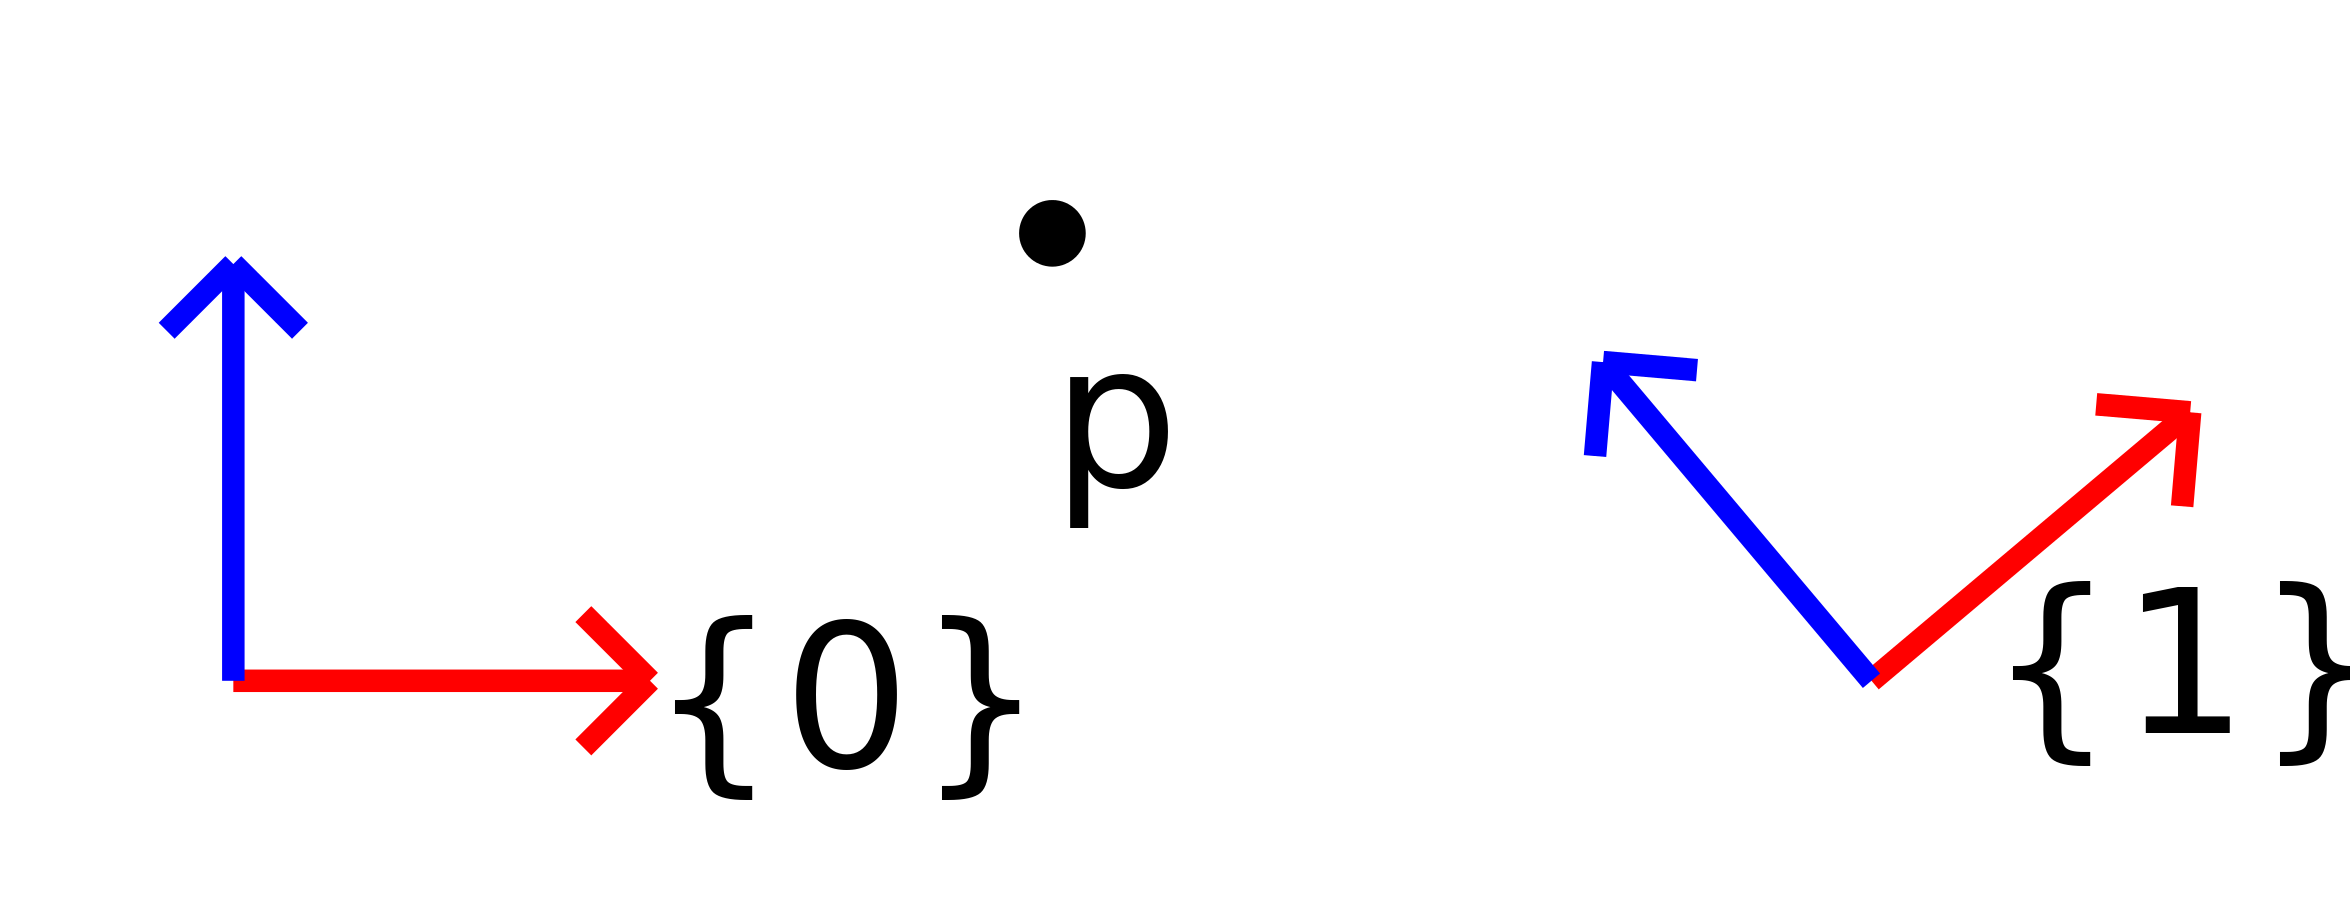
\includegraphics[scale=0.1]{generated_figures/frames_bg_pt.png}
\end{center}

\define{Vector}{
    A direction and magnitude that is free in space.  Among other things,
    vectors can describe offsets from a point, forces, or velocities. Just like a point, the
    direction of the vector depends upon in which frame it is referenced, but the magnitude
    remains constant in all frames. For example, in the figure below $\v{0} = \smcolvec{.7071\\-.
    7071}$ and $\v{1} = \smcolvec{0\\-1}$ both have a magnitude of 1.  
}
\begin{center}
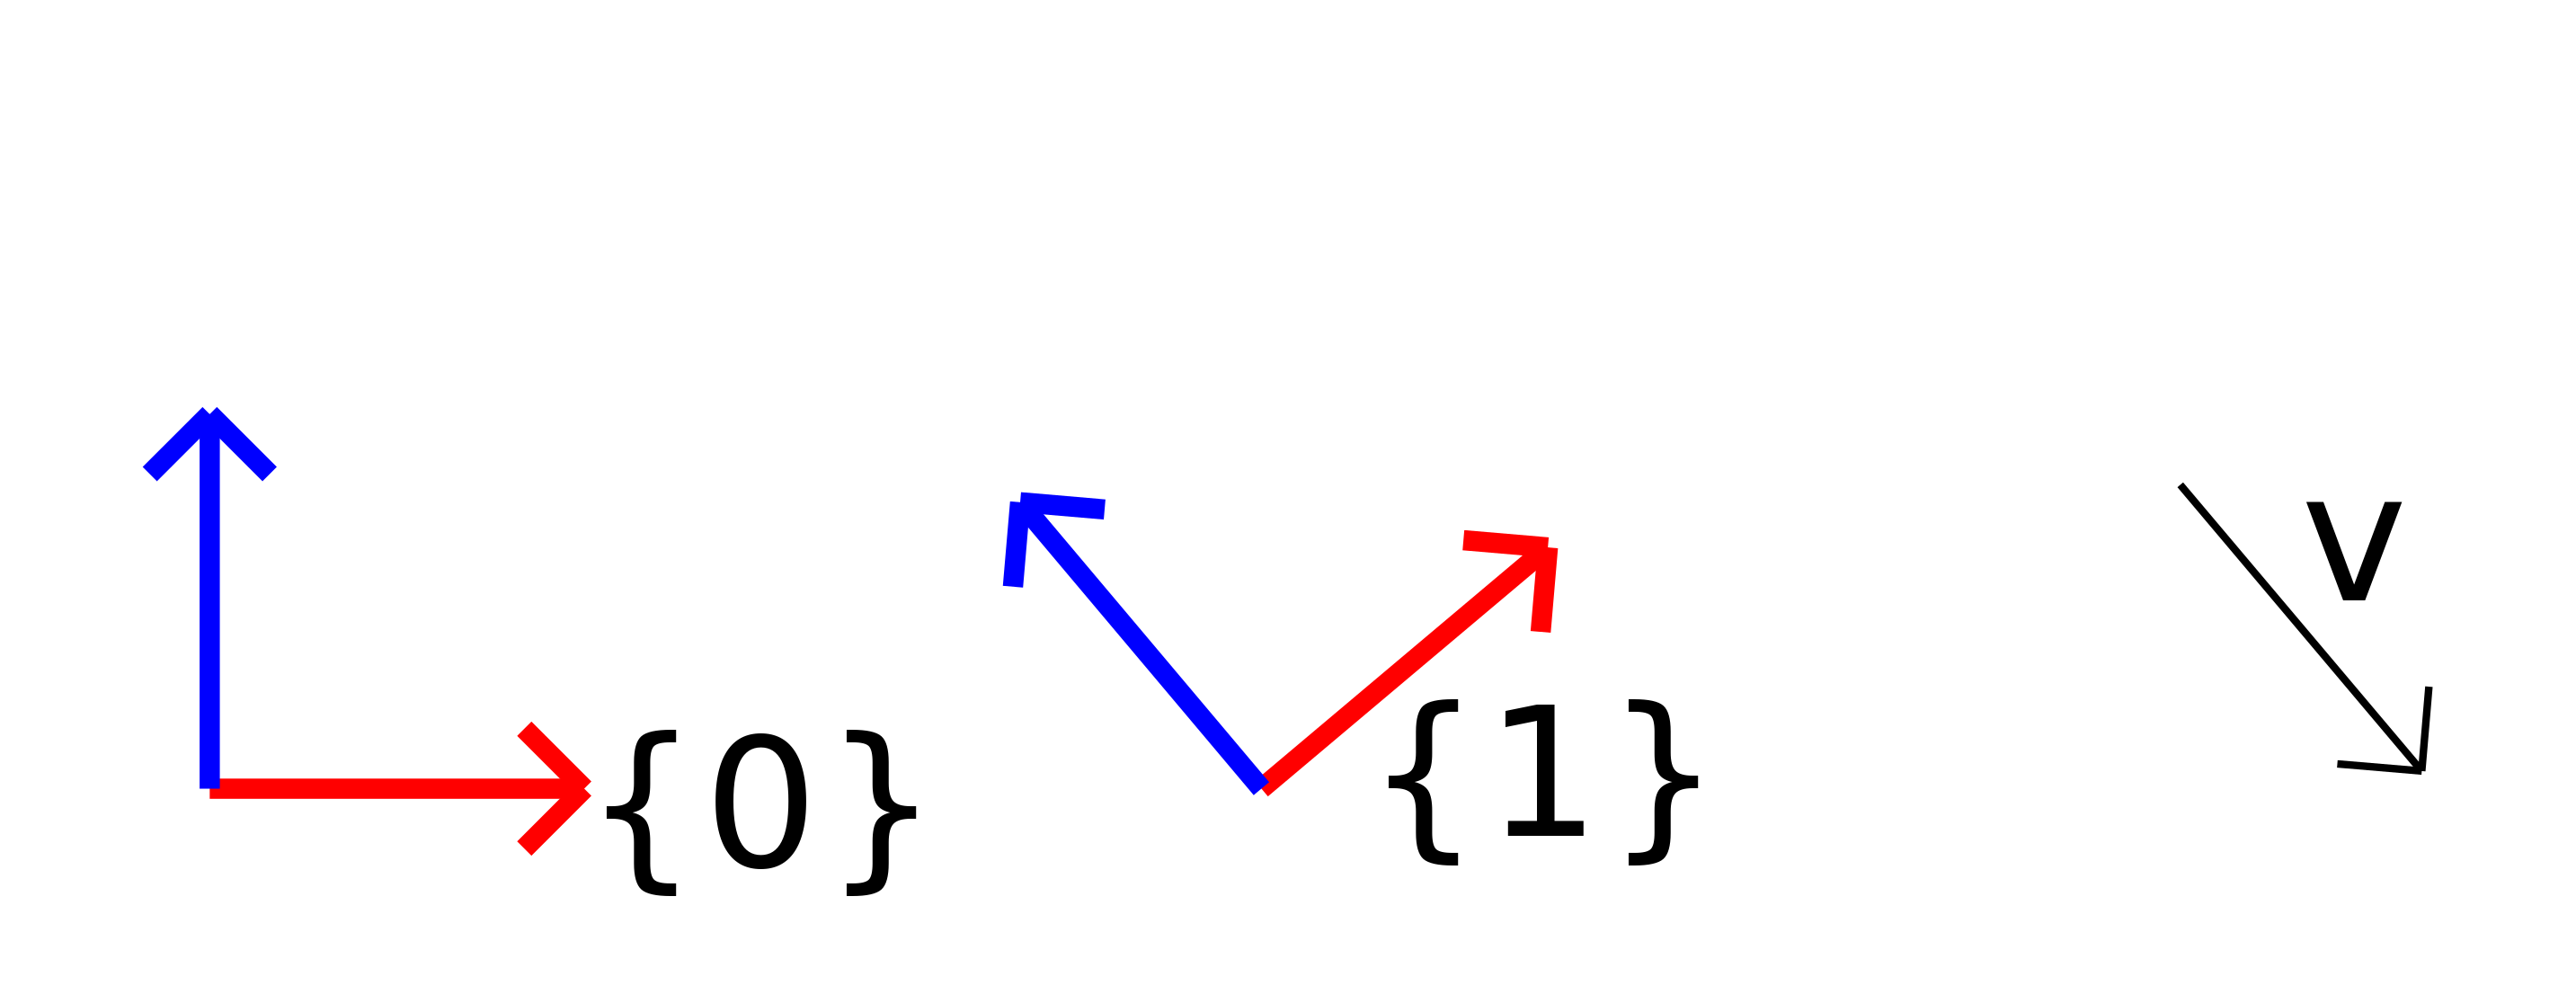
\includegraphics[scale=0.1]{generated_figures/frames_bg_vec.png}
\end{center}

\define{Rigid Body}{
    A collection of points where the distance between two points and the handedness of the points
    remains constant while the collection undergoes a displacement. 
}

\define{Rigid Motion}{
    A translation, rotation, or combination of the two that can be applied to
    a body without changing the distance between any two points in the body or 
    changing the handedness of the points.
}

\define{$\RR^2$}{
    Two-dimensional Cartesian space; can be parameterized by $x$ and $y$.
}

\define{SE(2)} {
    It is both 1) the space corresponding to position and orientation of a rigid body in two
    dimensions and 2) the set of rigid motions in two dimensions.
    It is usually parameterized by $x$, $y$, and $\theta$.
}

\define{Workspace}{
    The set of all points \p{} such that there exists
    some joint configuration which places a robot's end effector at \p{}.
}

\subsection{Robots and Robot Diagrams}

For the purpose of this class, a \textbf{robot} or a \textbf{linkage} is a
combination of \emph{links} (which are rigid bodies) and \emph{joints}, which
connect two links with a certain constraint on relative motion. Links are
generally represented by straight lines in robot diagrams. The two
categories of joints we will use in this class are \emph{rotational} and
\emph{prismatic} joints.

\define{Revolute Joint}{
    Creates an angular offset between two adjacent links.  This offset is
    typically notated as $\theta$, with a subscript that matches the joint index
    or name.  Positive rotations go from the x axis towards the y axis (i.e.,
    they follow the right hand rule). They are drawn as follows in robot
    diagrams: 
}
\begin{center}
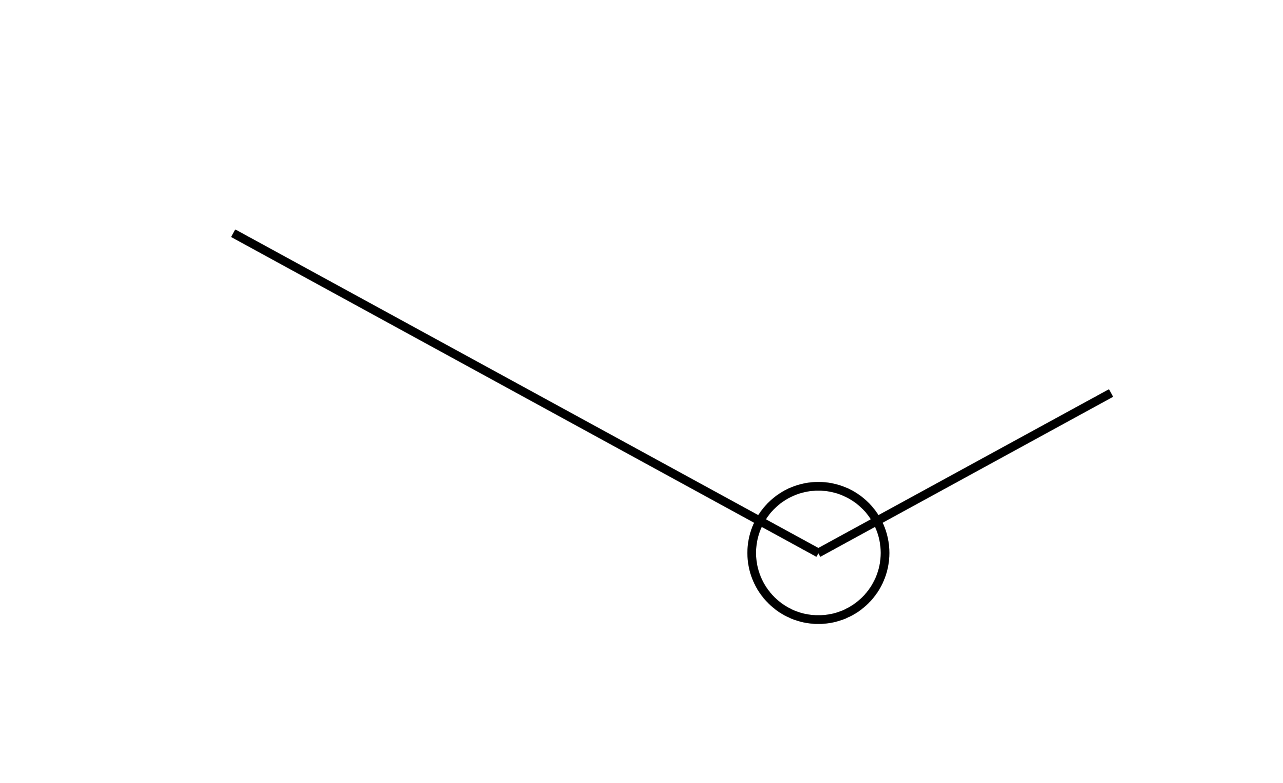
\includegraphics[width=1.5in]{generated_figures/bg_rot_joint_diagram.png}
\end{center}

\define{Prismatic Joint}{
    Creates a translational offset between two adjacent links along a single axis. The notation
    for this offset varies. We will refer to this as $d$ with a subscript to match the joint
    index or name, but in a robot with both rotational and prismatic joints sometimes $\theta or
    q$ is used for any joint.  They are drawn as follows in robot diagrams.
    Note that this figure represents two separate links with one prismatic joint
    in between with a total length is $l_1 + l_2 + d$; however, depending on the
    system, $l_1$ and $l_2$ may be omitted and just combined into $d$. You can use either
    convention, but be sure to label any diagrams clearly.
}

\begin{center}
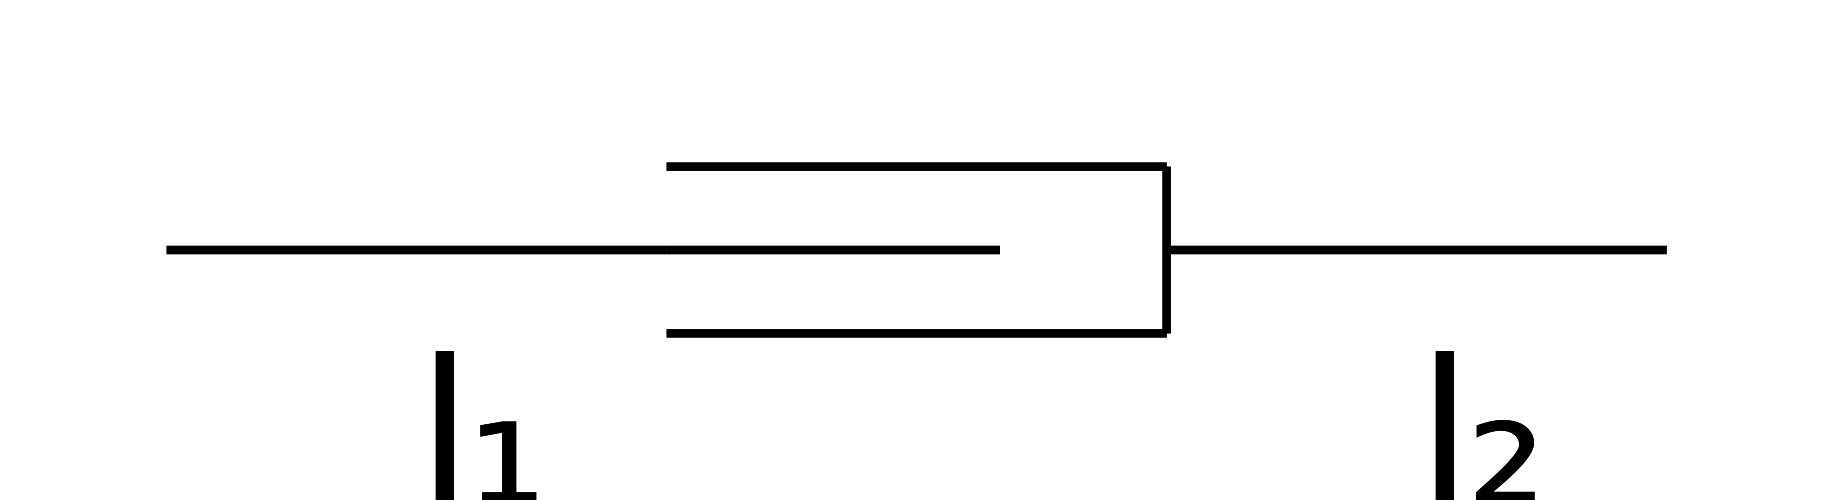
\includegraphics[width=1.5in]{generated_figures/bg_prism_joint_diagram.png}
\end{center}

\define{Kinematic Chain}{
    An $n$-joint kinematic chain is a robot consisting of $n+1$ links and $n$ joints, connected
    in series.  If the robot is attached to the world, the first link is called the base link.
    Often, the first link has zero length and is omitted. Many of our examples will have a zero 
    length base link or "no base link." Joint $i$ connects links $i-1$ and $i$ and joint $i$ 
    moves link $i$.  It is also possible to have a free floating robot of $n+1$ links connected 
    by $n$ joints. 
}

\define{Fixed Base}{
    Drawn as follows, this represents a rigid point of attachment to the world.
}
\begin{center}
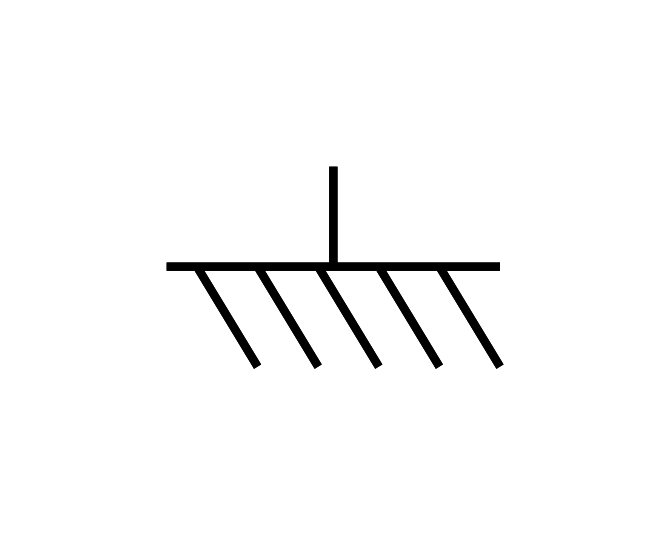
\includegraphics[width=0.75in]{generated_figures/bg_base_diagram.png}
\end{center}

\define{End Effector}{
    Drawn as follows, this represents a gripper or other end effector attached
    to the end of a robot link (or directly to the output of a joint). We
    generally do not consider the end effector to add a degree of freedom to the
    robot, as it does not take part in the overall kinematics.
}
\begin{center}
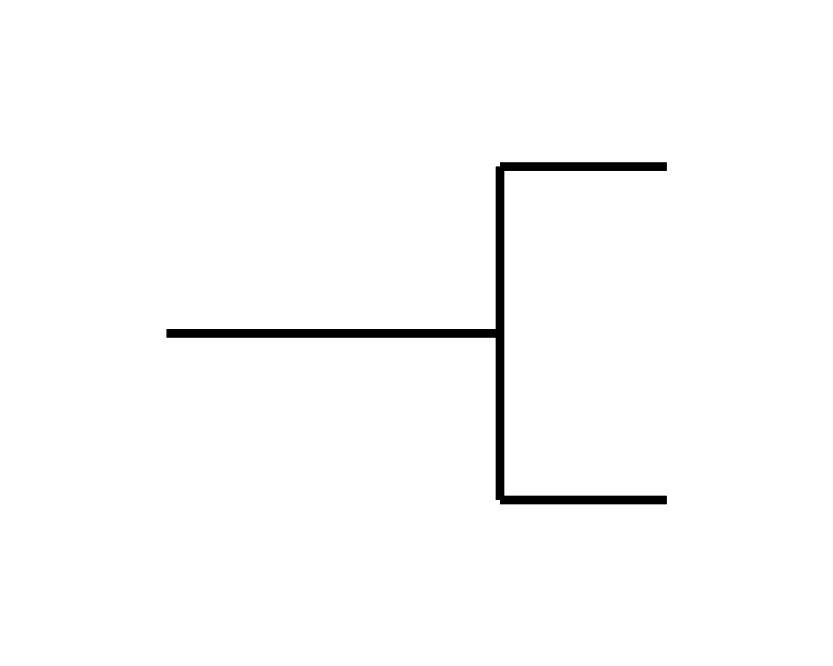
\includegraphics[width=0.75in]{generated_figures/bg_endeffector_diagram.png}
\end{center}

% directions

\define{Frame Conventions}{
    We define a \emph{base} frame as a coordinate frame at the point where the robot is fixed to
    the world, labeled \frame{0} (NOTE: in the OLI material, this frame is omitted).
    We also define a coordinate frame at the base of each link (the \emph{proximal}
    frame for that link).  Optionally, we can also define a frame at the \emph{end}
    of each link, where the next link is attached by a joint; this is the \emph{distal}
    frame. Note that this is also omitted in the OLI material, but is used in this
    assignment to help define the order of all intermediate transformations.
    The convention in this class will be that the $x$ axes of these frames points
    from the base to the end of the link. End effectors of planar robots will have a frame
    defined at the attachment point to the link, and the $x$ axes will point \emph{out} of the 
    gripper (i.e., this frame will usually match the distal frame of the connecting
    link). Positive angles of rotation will be counter-clockwise (from the $x$
    axis towards the $y$ axis). Below are several simple robots demonstrating
    these conventions.
}

\begin{center}
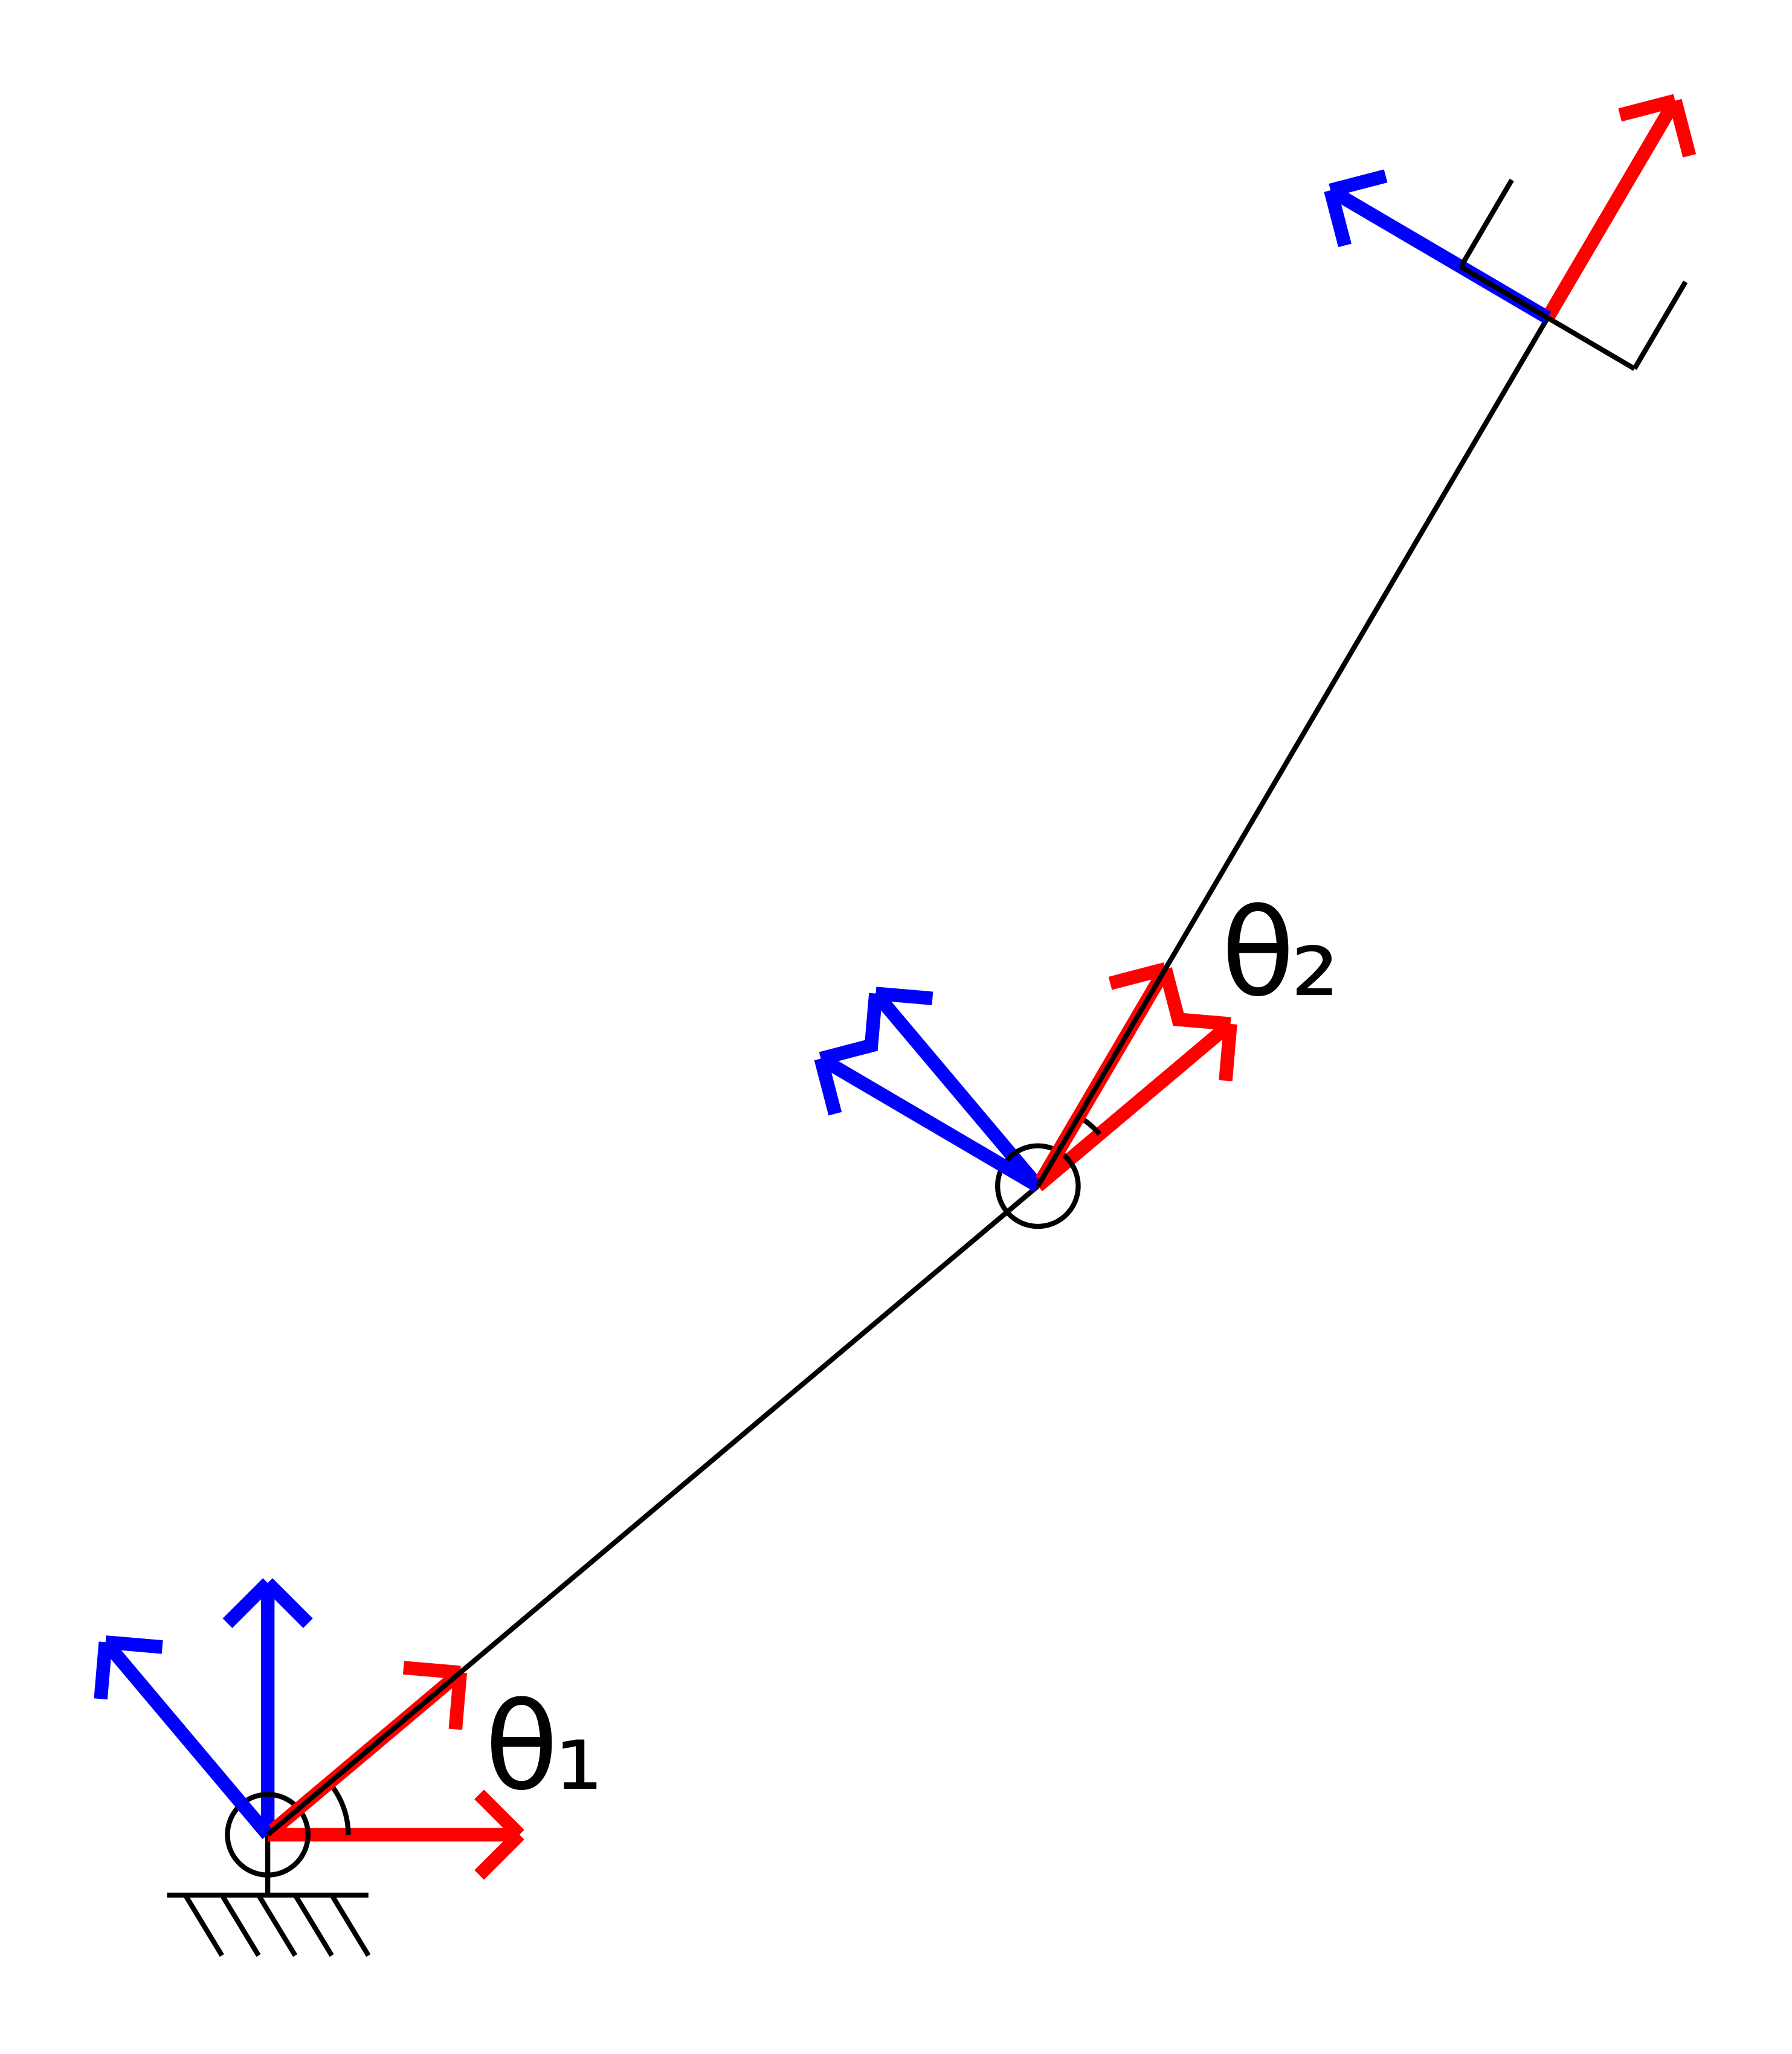
\includegraphics[scale=0.05]{generated_figures/bg_example_diagram_1.png}
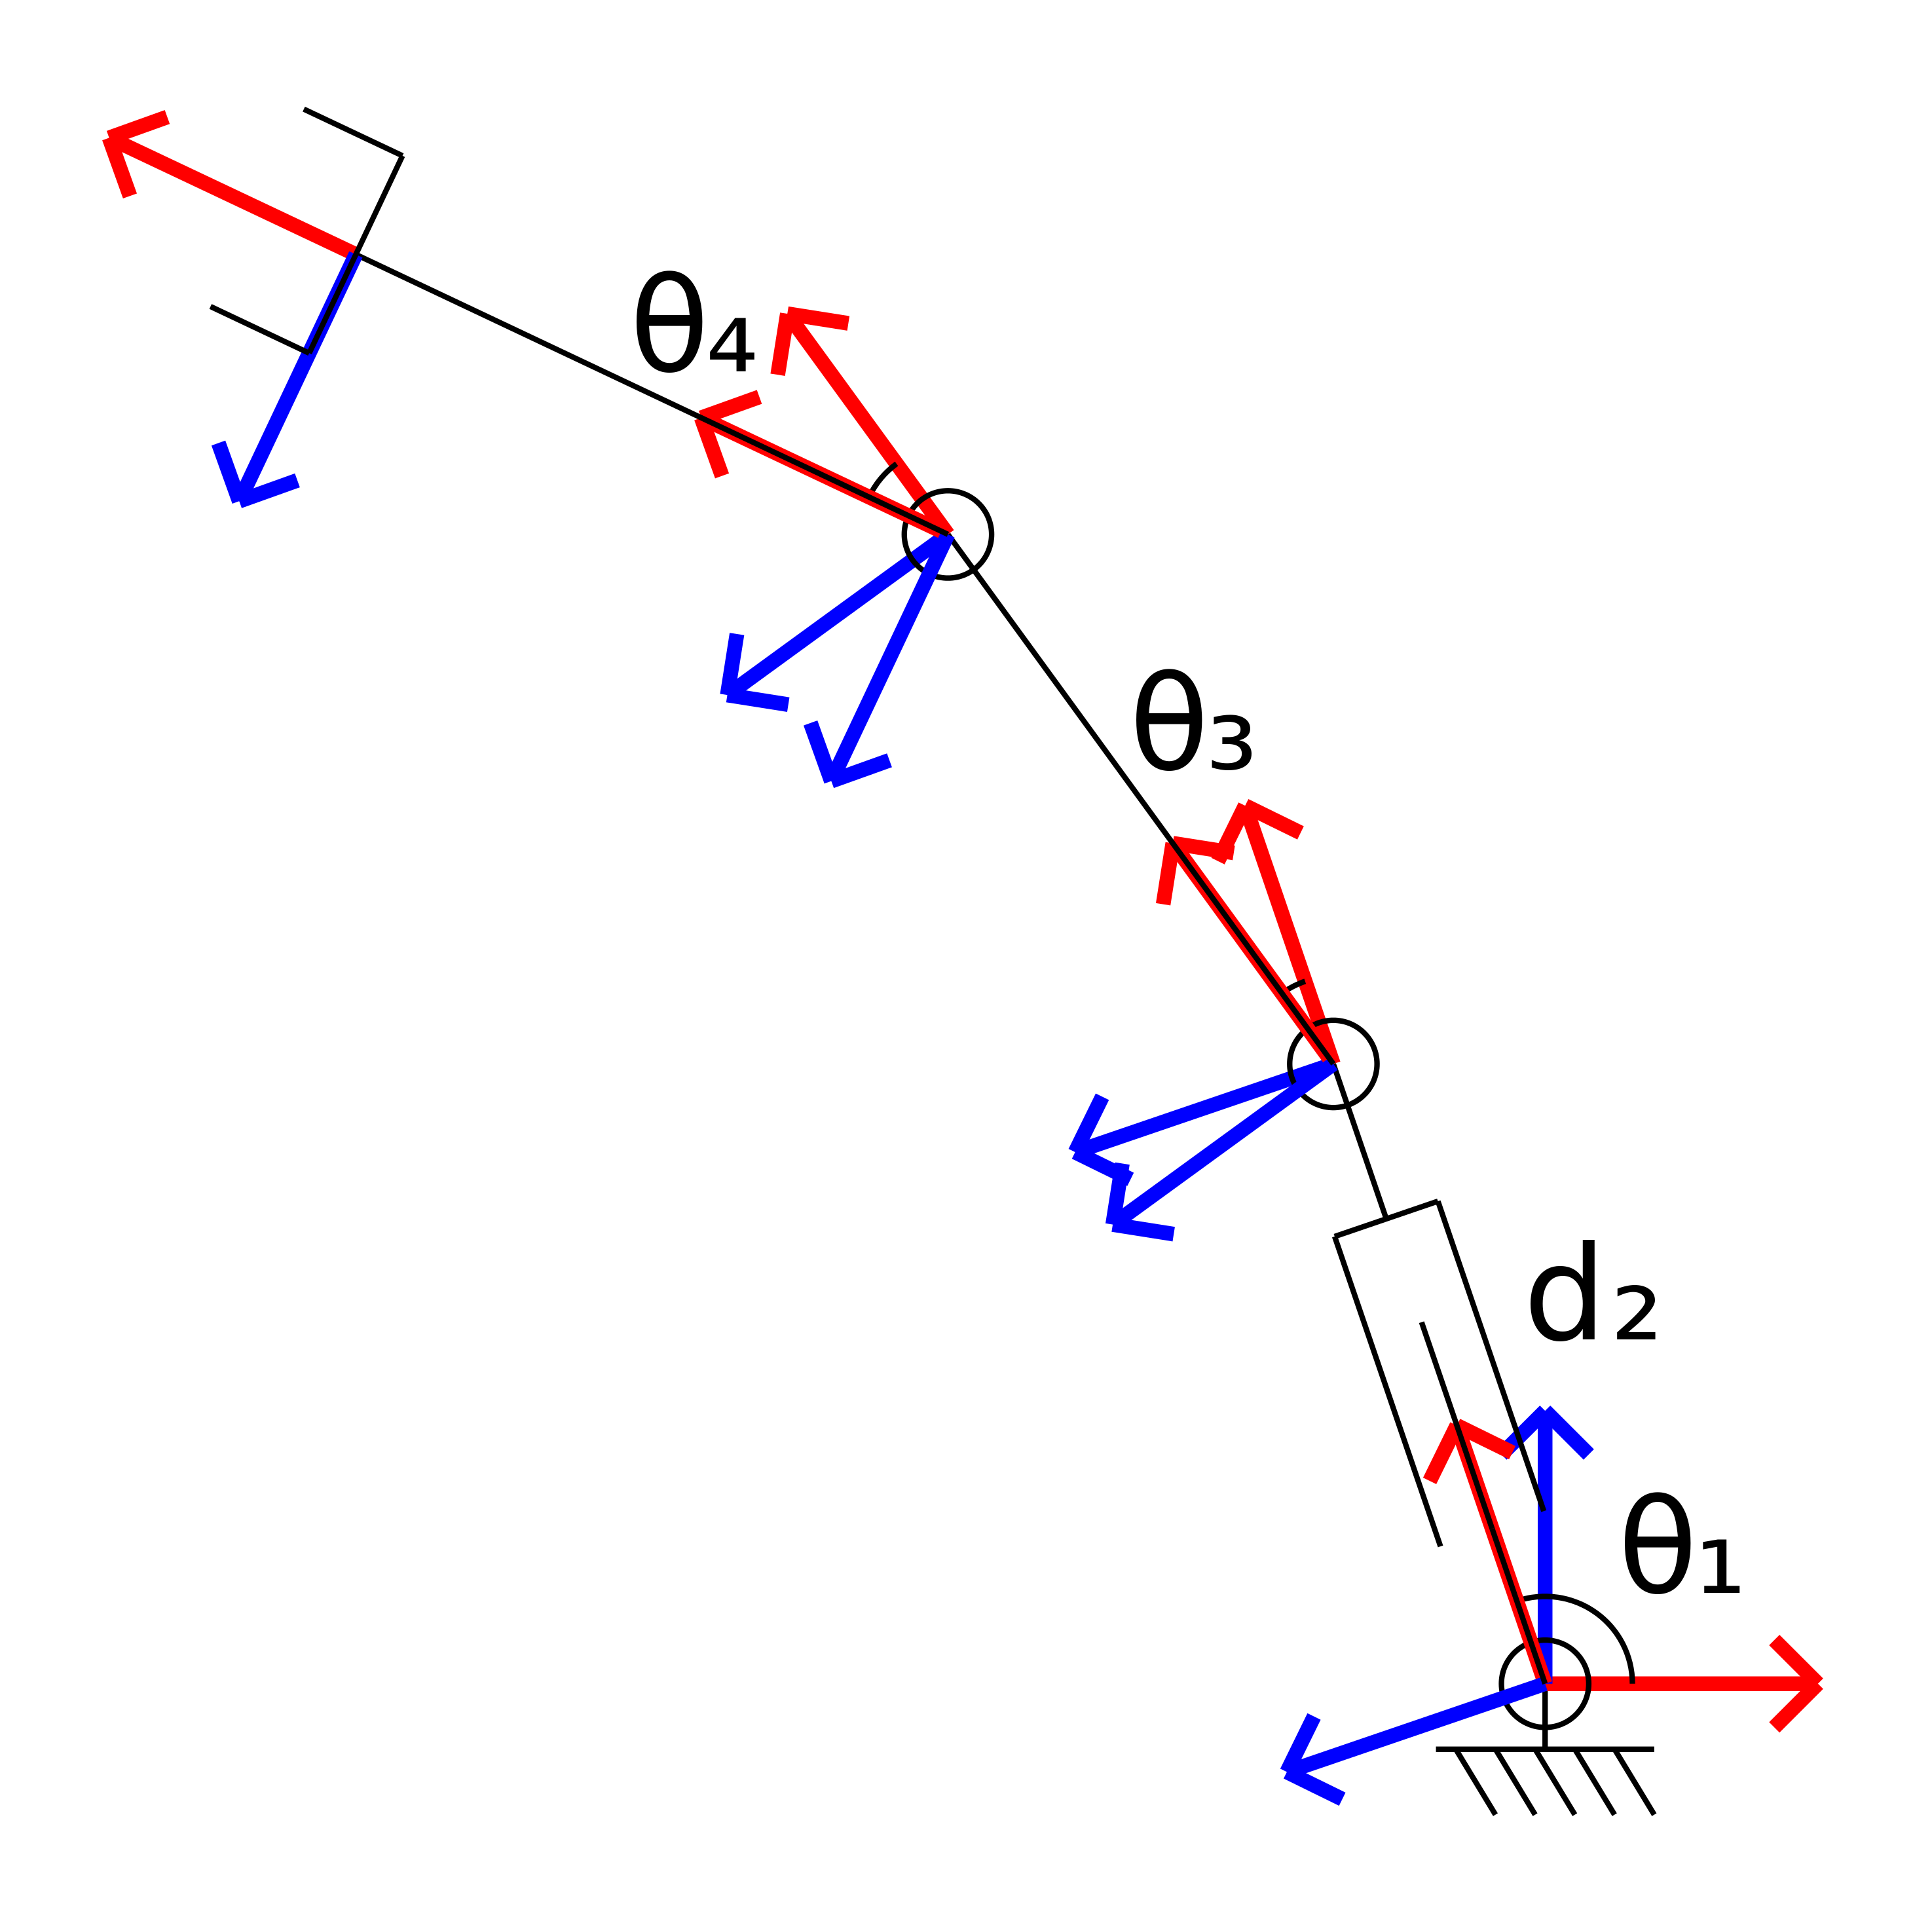
\includegraphics[scale=0.05]{generated_figures/bg_example_diagram_2.png}
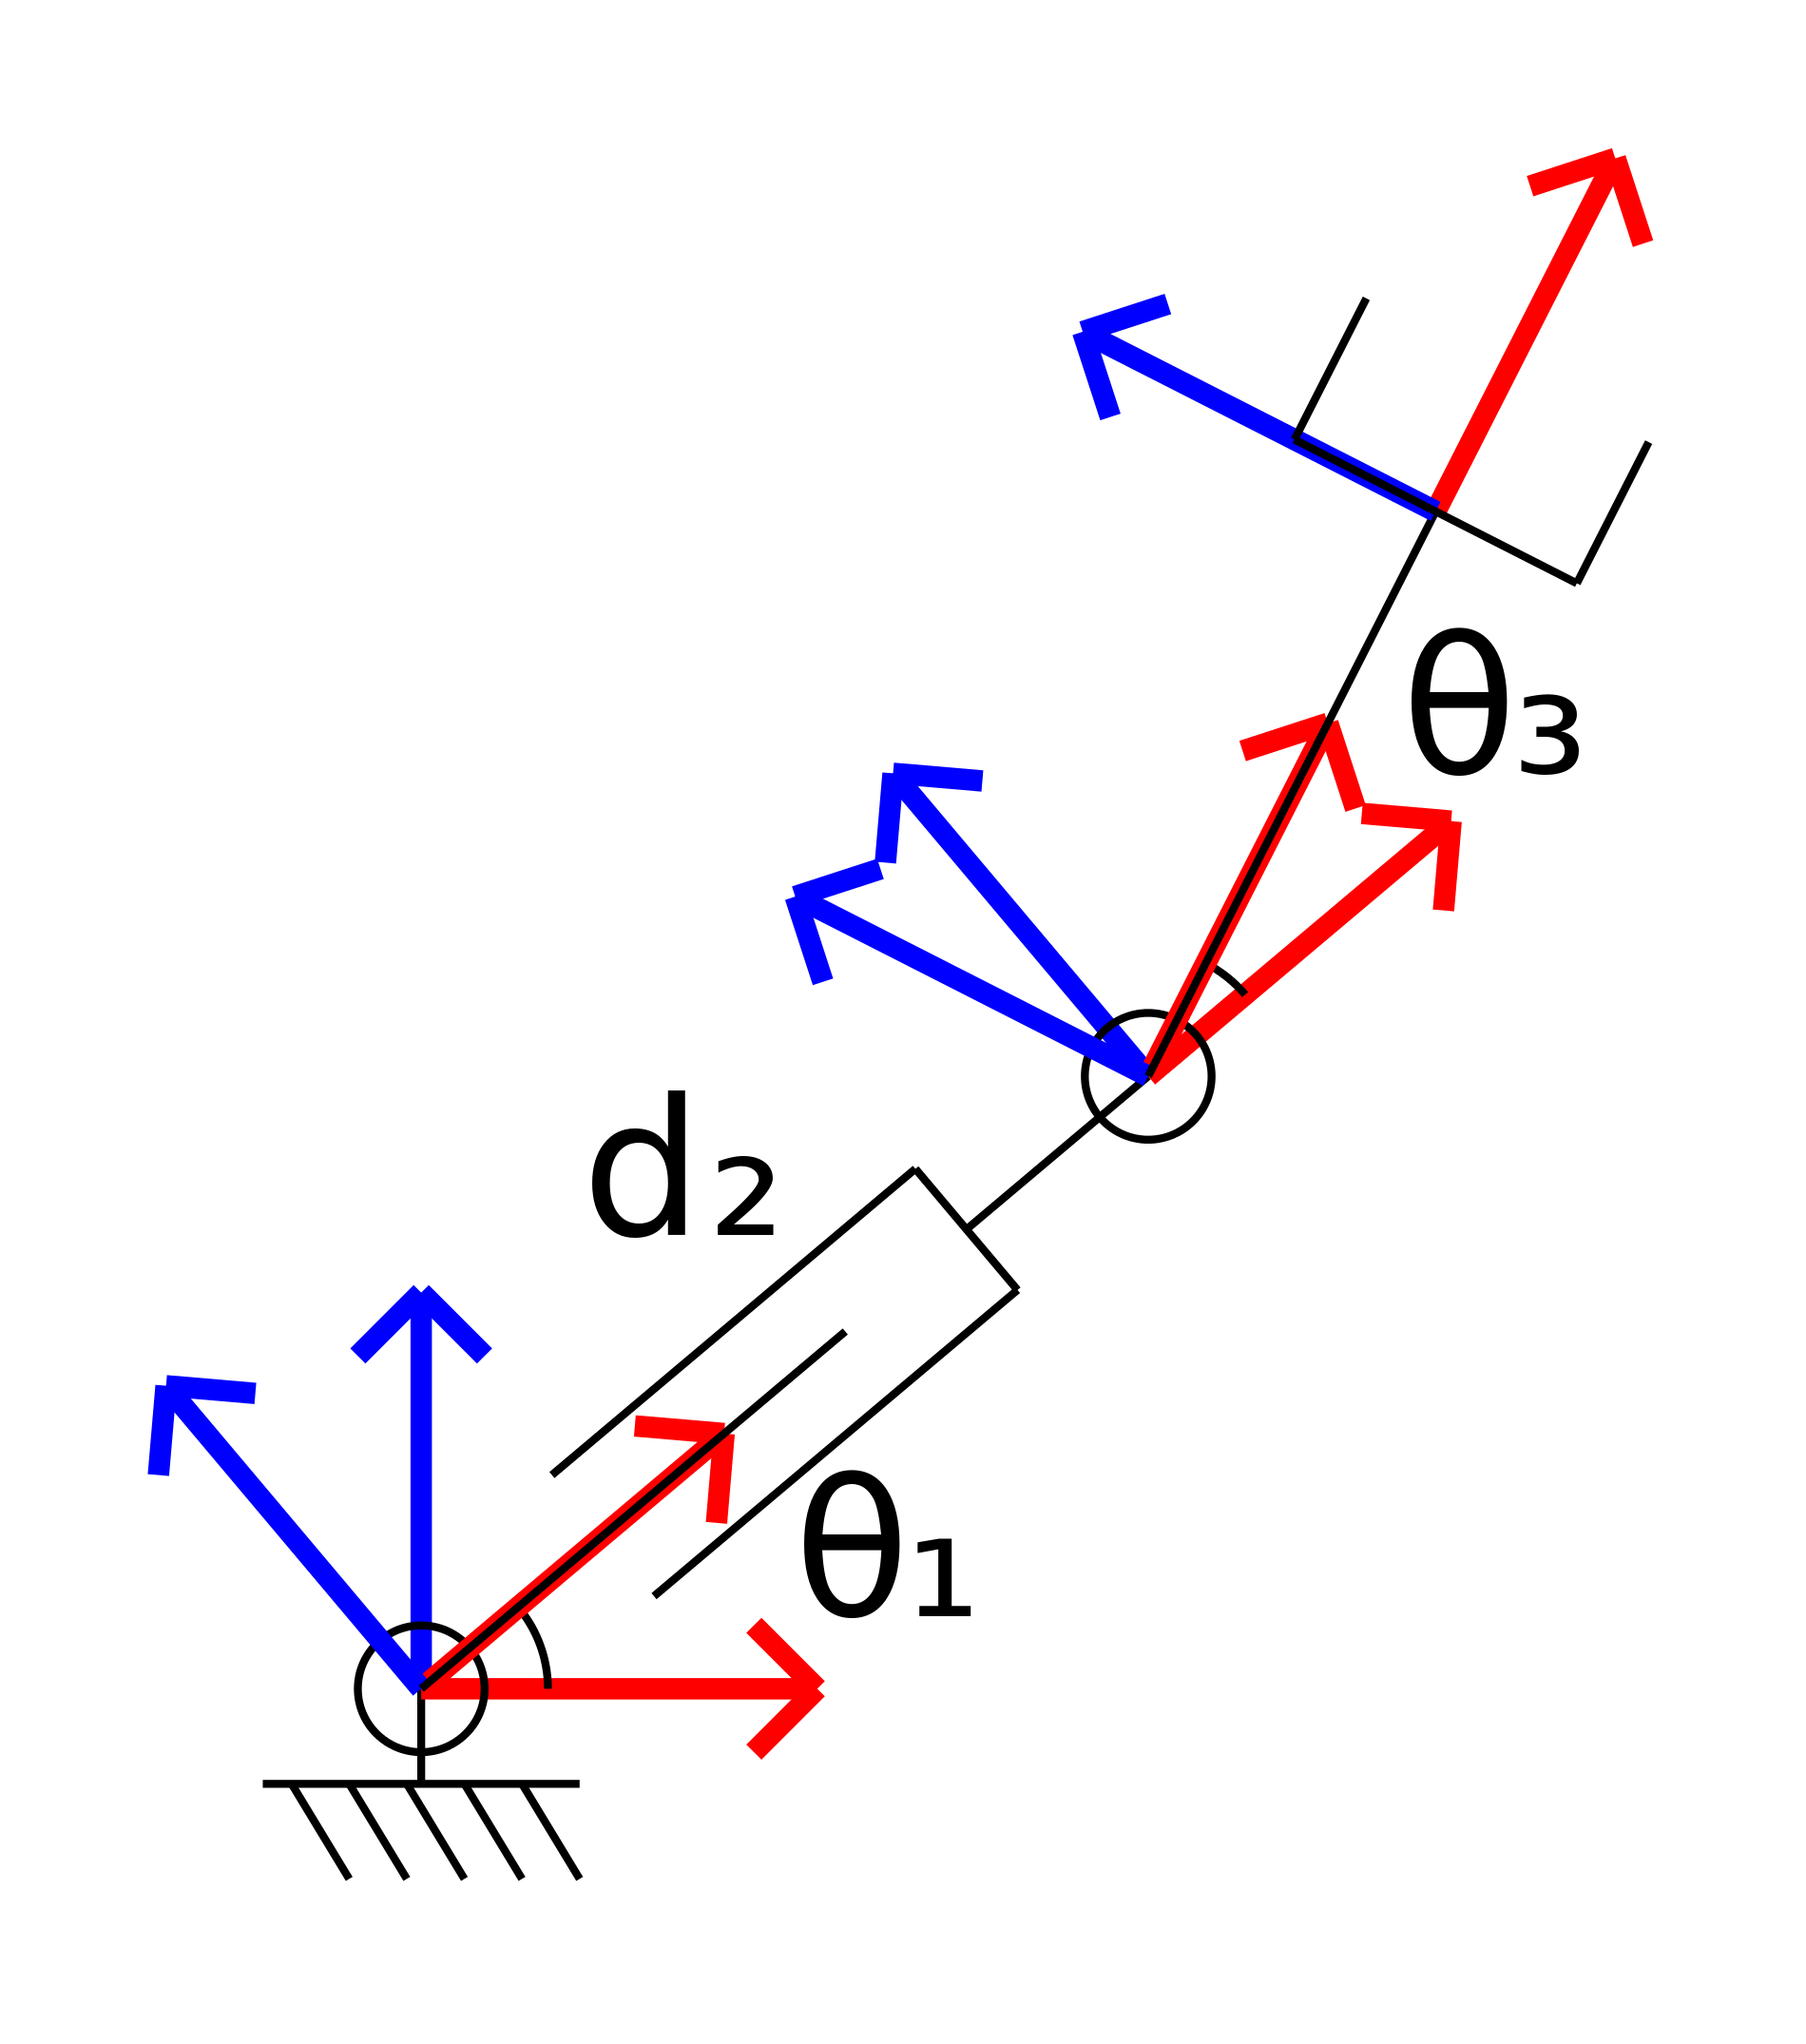
\includegraphics[scale=0.05]{generated_figures/bg_example_diagram_3.png}
\end{center}

\subsection{Degrees of Freedom}

In robot kinematics, a system's \emph{degrees of freedom}, or \emph{DOF}, is the number
of parameters needed to completely define a particular configuaration.  For example:

\begin{itemize}
    \item A point in two dimensions (i.e., $\RR^2$) has 2 DOF, since \smcolvec{x\\y} completely
        defines the point's configuration.

    \item A rigid body in the plane has 3 DOF, since \smcolvec{x\\y\\\theta}
        completely defines its position and orientation.

    \item An fixed-base n-joint kinematic chain in SE(2) has $n$ DOF, since $n$
    parameters for the joints completely define the robot's configuration.  If
    the robot isn't attached to the base frame, the base link can move freely
    (in $x$, $y$, and $\theta$), and the robot has $n + 3$ DOF.
\end{itemize}

\subsection{Rigid Motions / Transforms in Two Dimensions}

There are two basic types of motions/transformation we are concerned with:
rotations and translations. Rotations are represented with matrices, and
translations are represented by vectors.  These can be combined into compound
motions/transformations.

Rotations and translations are used for two different concepts.  The first is
the motion of a point or rigid body within a coordinate frame:

\begin{center}
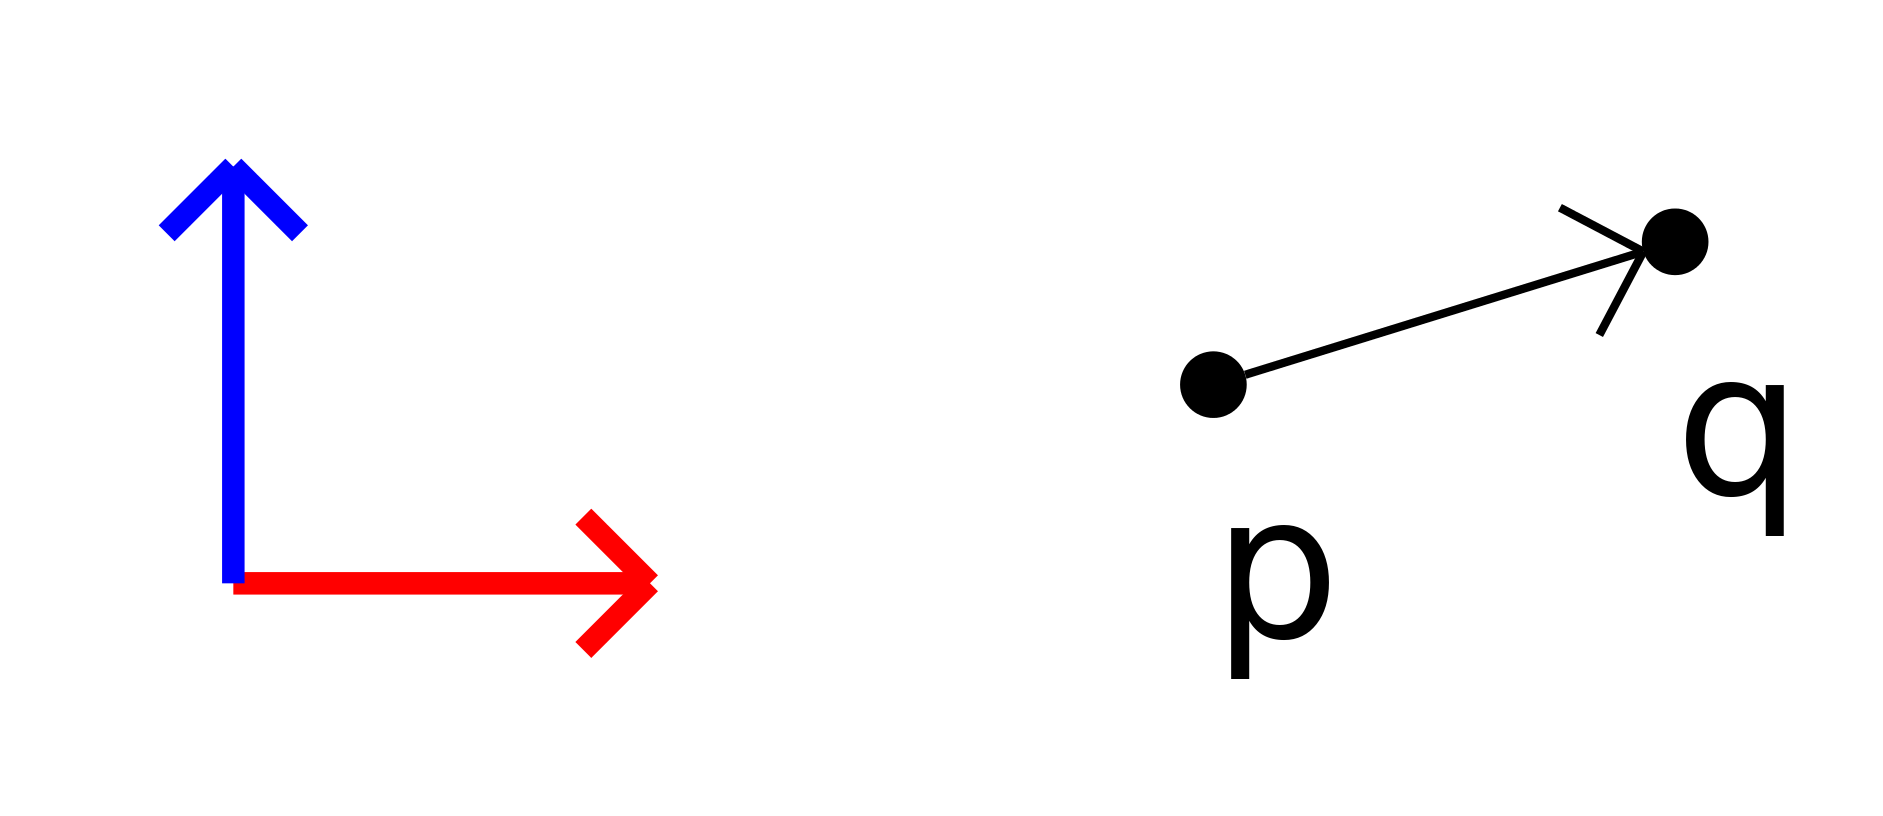
\includegraphics[scale=0.1]{generated_figures/bg_motion.png}
\end{center}

The second concept is a \emph{transform} between two coordinate frames. In
other words, if you have the coordinates of a point or vector in \frame{0}, what
are the coordinates of this same point or vector in \frame{1}:

\begin{center}
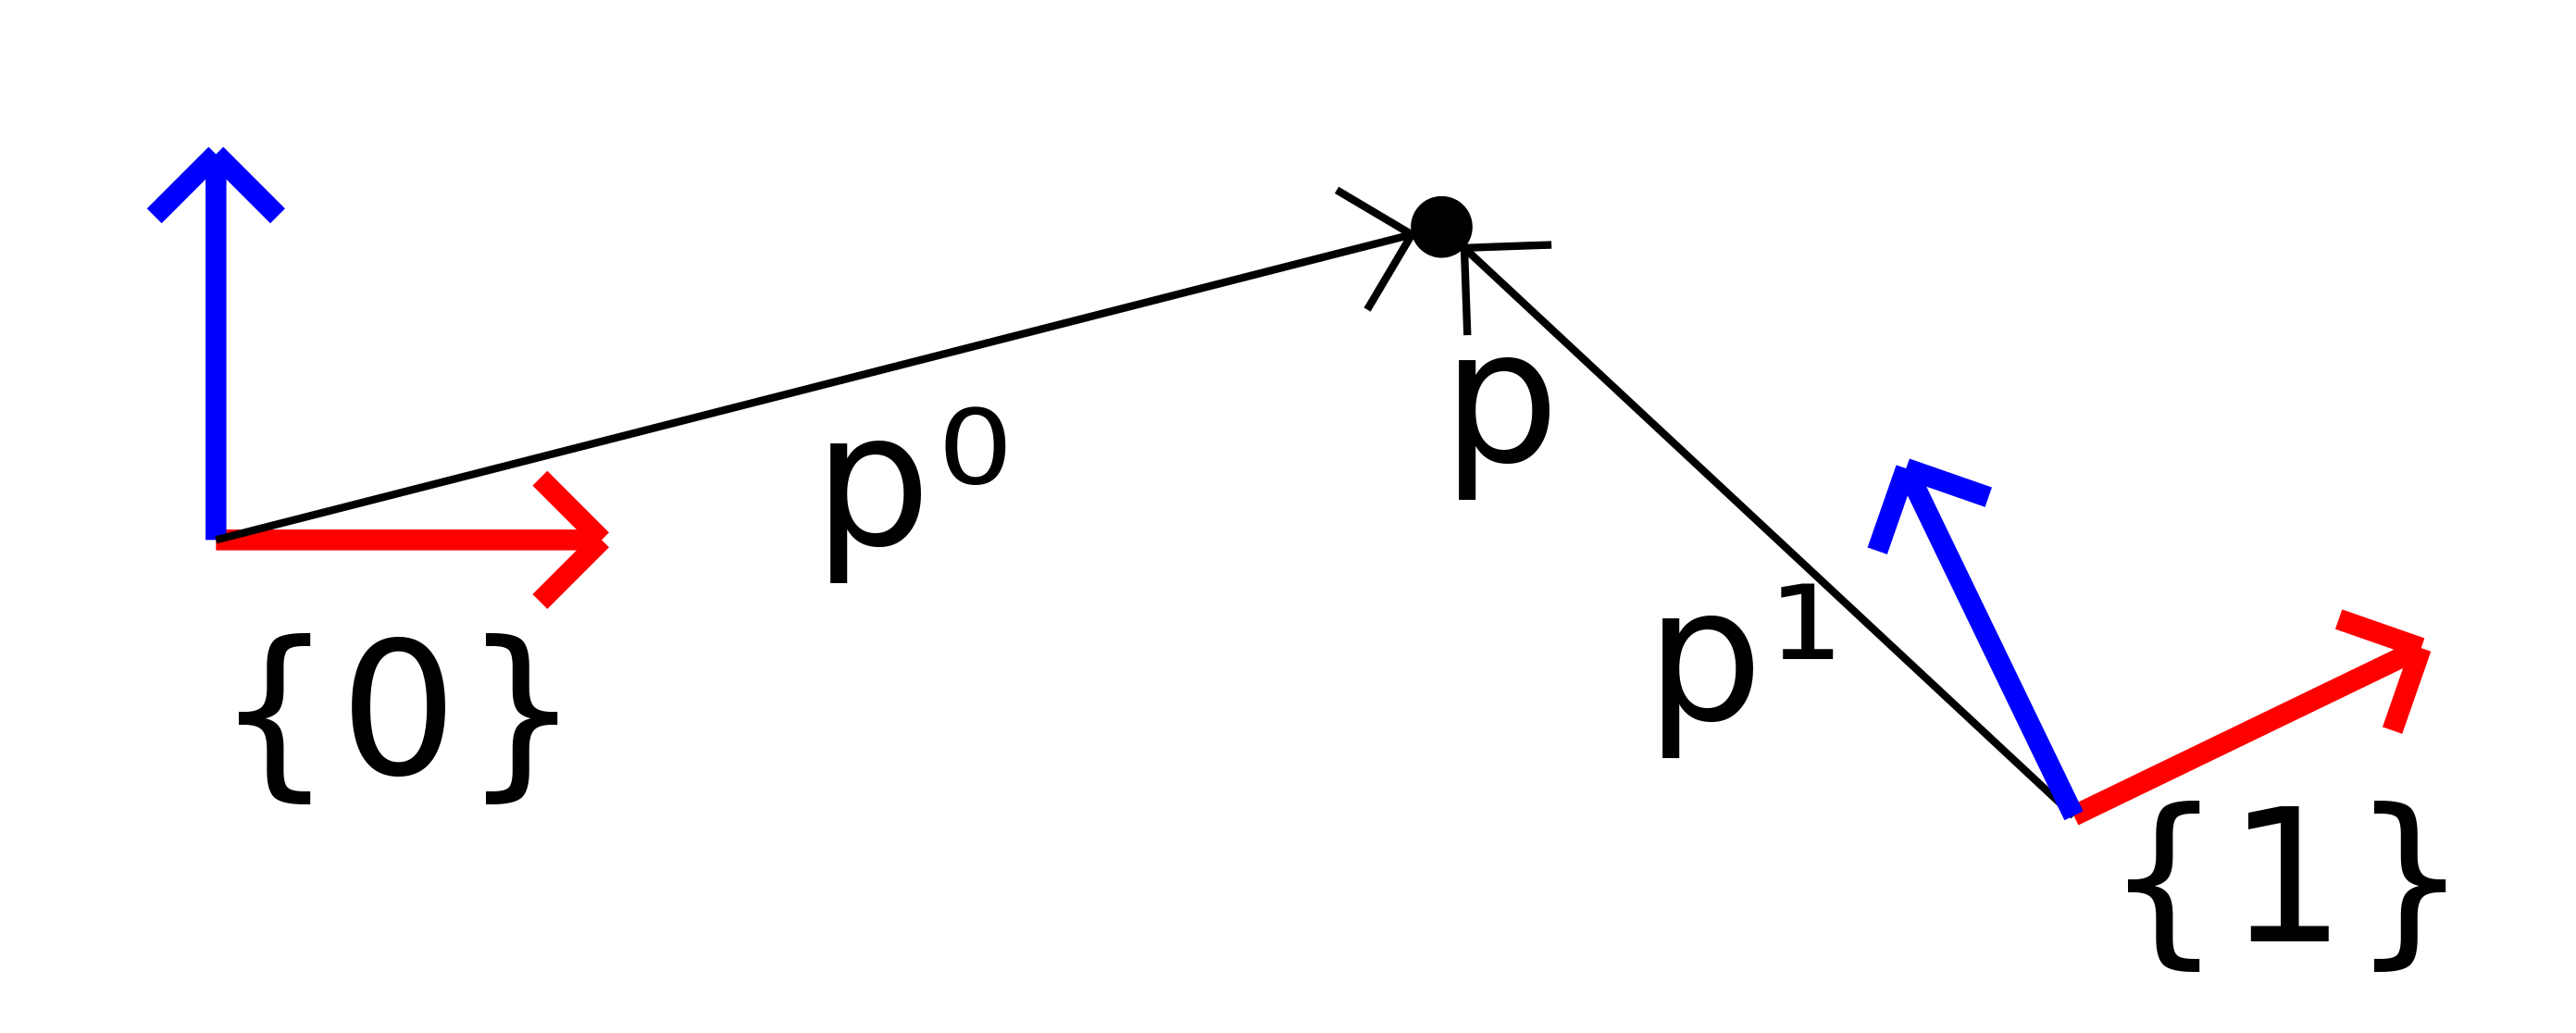
\includegraphics[scale=0.1]{generated_figures/bg_transform.png}
\end{center}

Notationally, transformations follow the convention of a superscript and a
subscript, to describe which frames are transformed between. A transform
$\transform{T}{b}{a}$ between two frames has several interpretations (notice
the order of the superscripts in each case).
\begin{itemize}
  \item The motion that moves \frame{a} to \frame{b}.
  \item \frame{b} as represented in \frame{a}.
  \item The transform that changes the representation of a point or vector from
    \frame{b} to \frame{a}.
\end{itemize}

\vspace{0.2in}
Note that the motion between two frames is the opposite of the transform that
changes point representation between these frames. This is something which can
often lead to errors! A good rule of thumb is that the top number always represents what
frame this motion/transform is represented in.  Here, the transform is in
the frame of reference \frame{a}. Below, we explicitly consider translations, rotations, and combined motions.

\subsubsection{Translation}

% Drawing of frames i and j, where j is offset by \smcolvec{\Delta x\\\Delta y}
\begin{center}
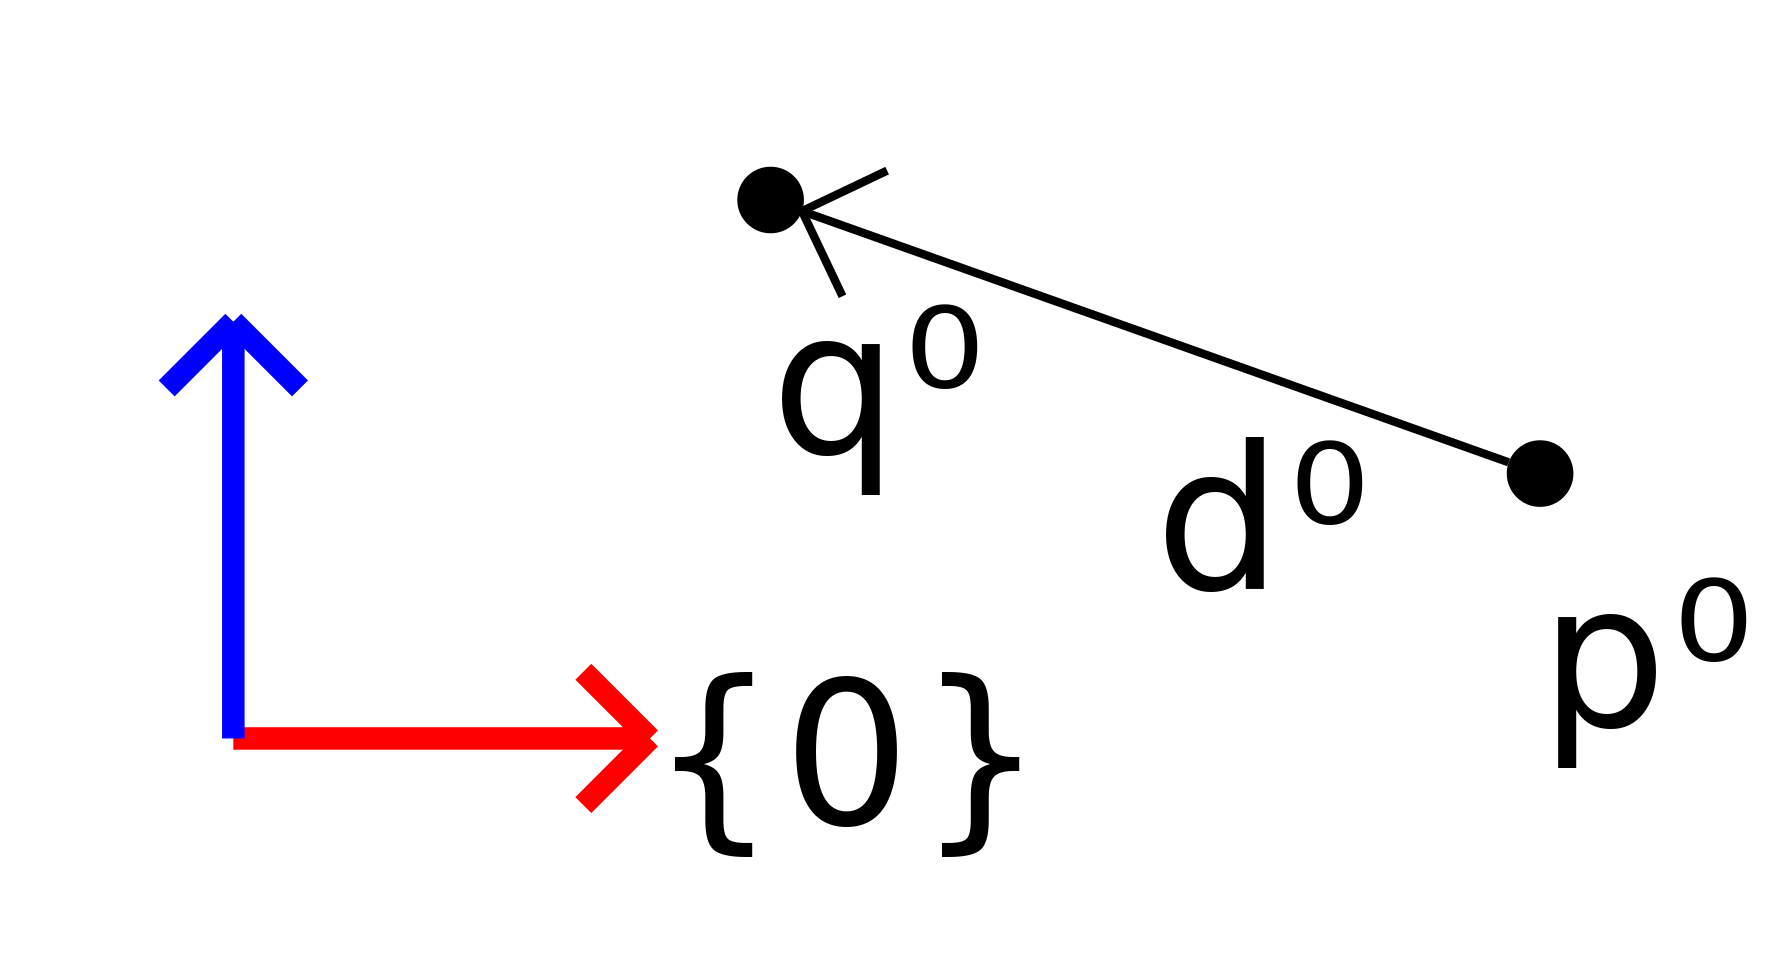
\includegraphics[scale=0.09]{generated_figures/bg_translation_motion.png}
\hspace{0.5in}
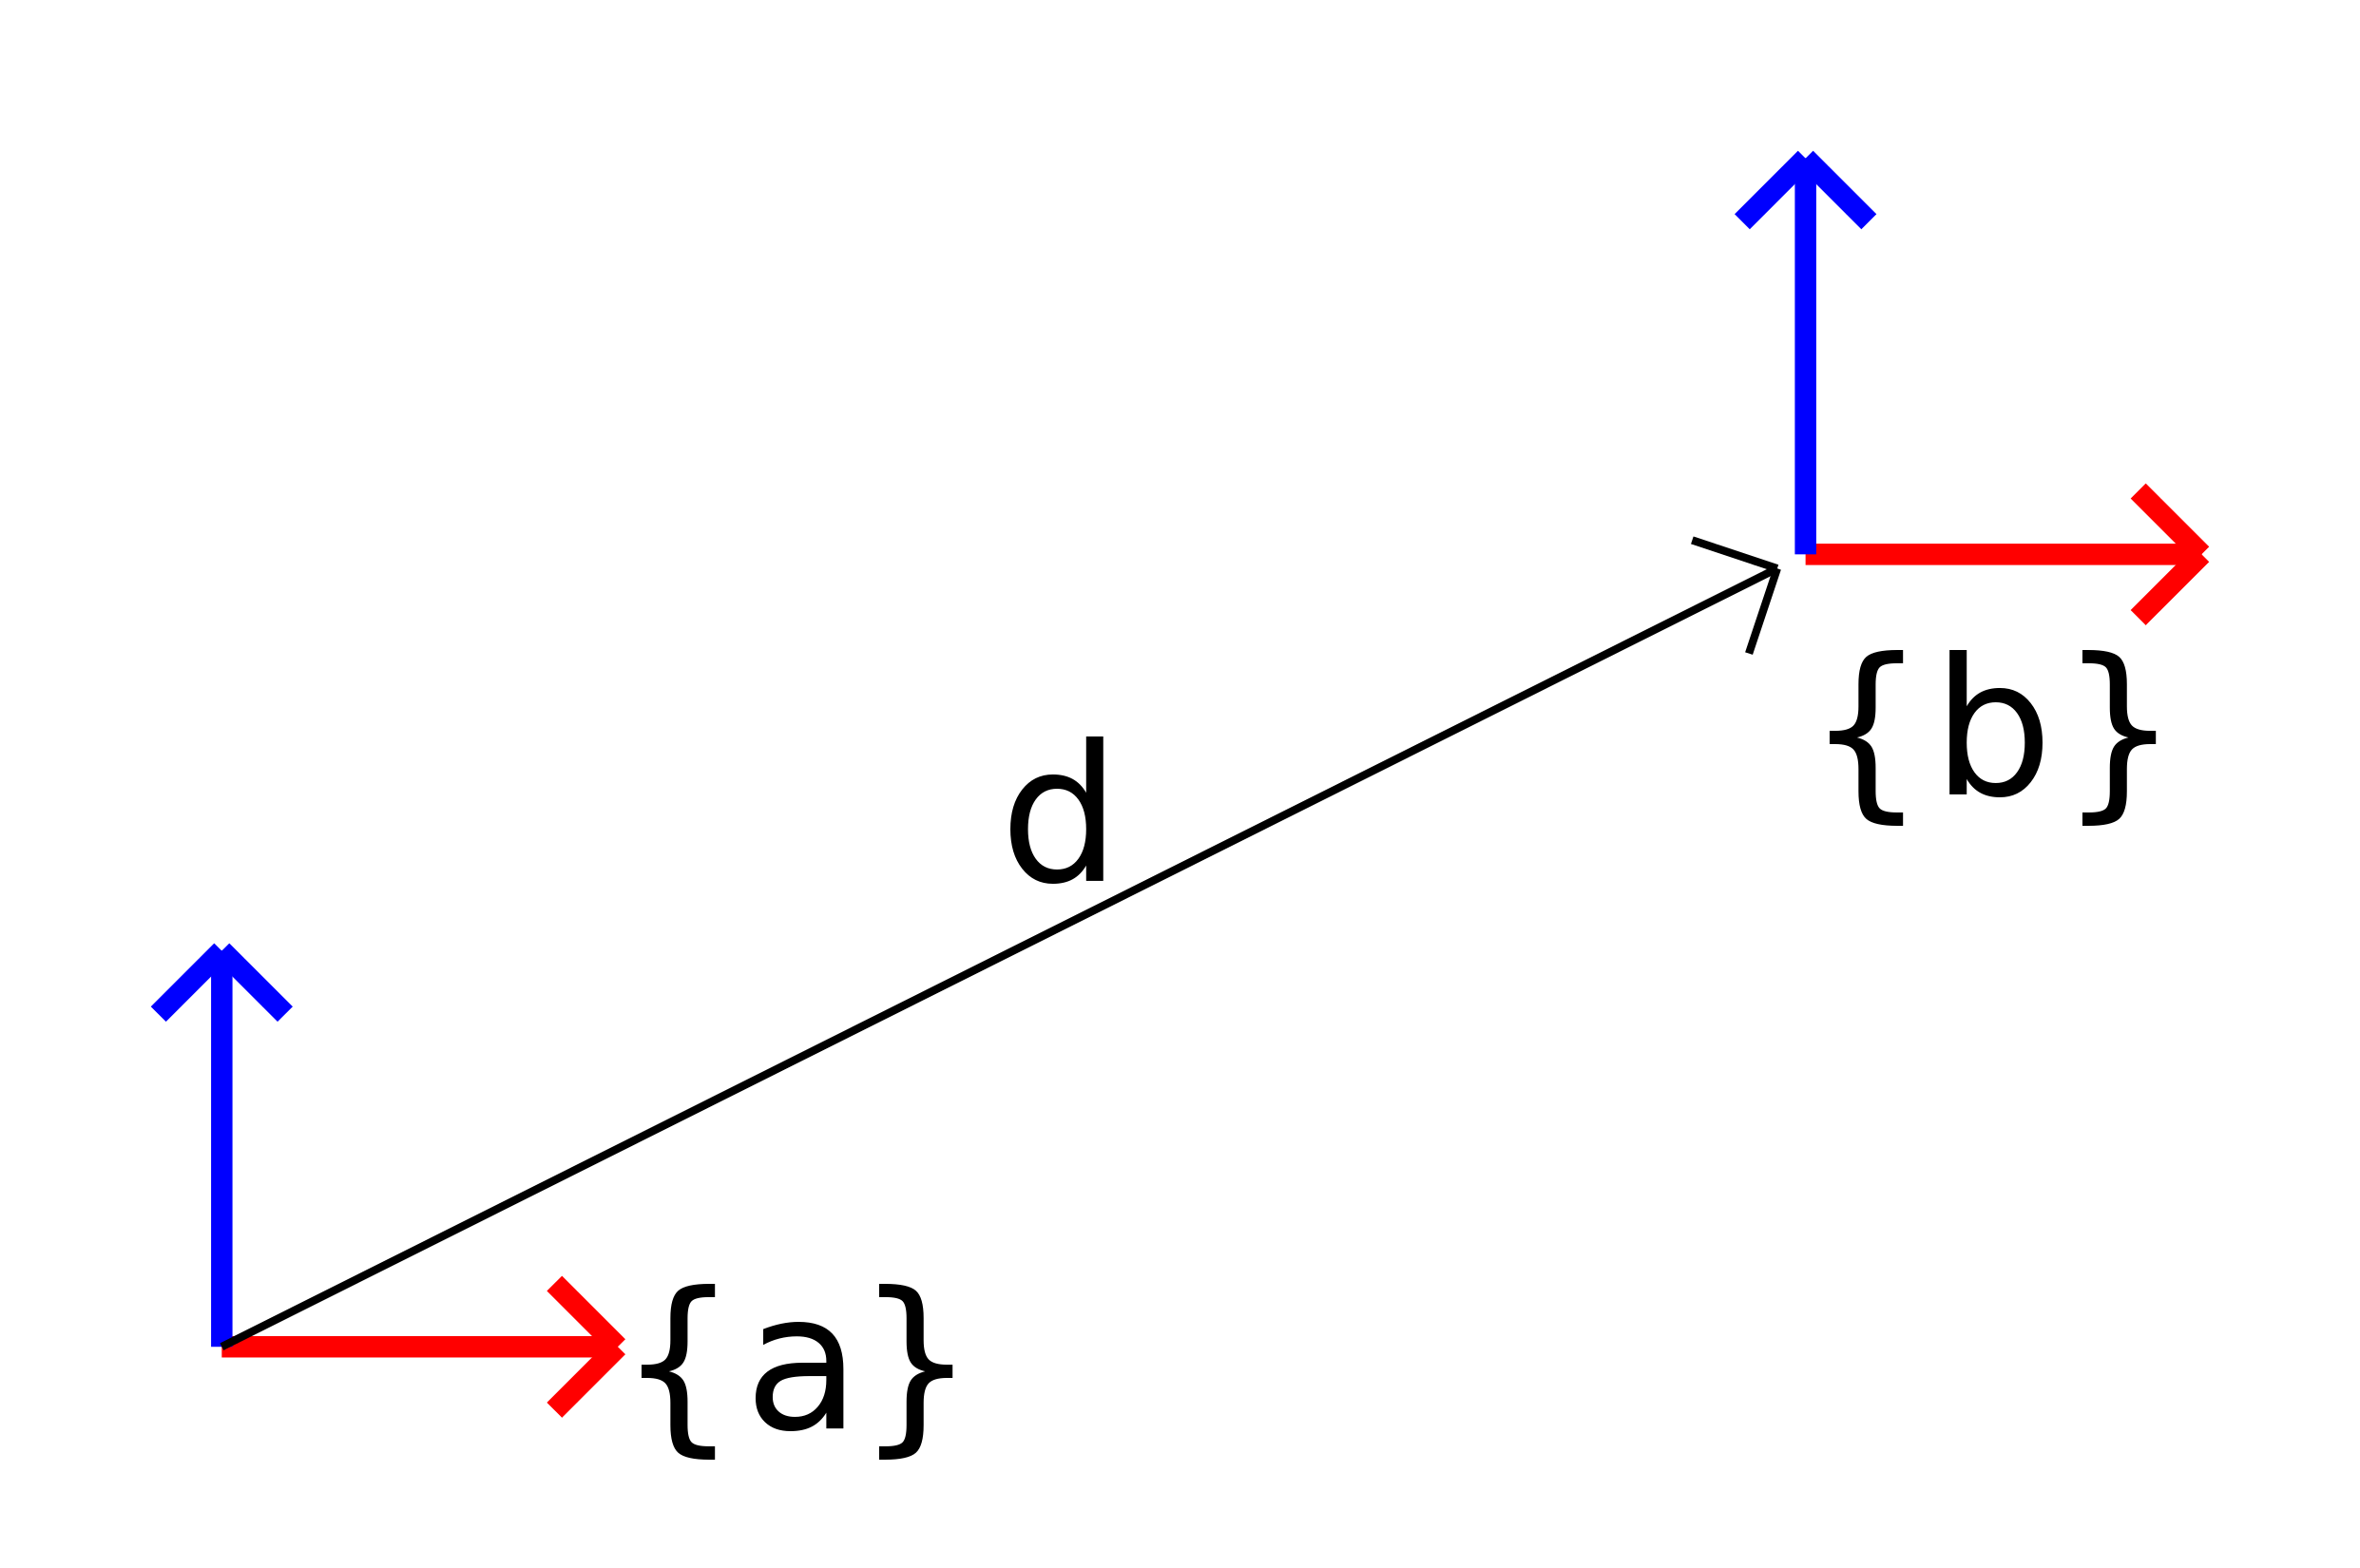
\includegraphics[scale=0.09]{generated_figures/bg_translation.png}
\end{center}

A translation $\t{}{} = \smcolvec{\Delta x\\\Delta y}$ expresses a change in
position of a point or rigid body, or a position offset between coordinate
frames. In terms of rigid motions, translating a point is the geometric addition of two
positions; above left, $\transform{q}{}{0} = \p{0} + \t{}{0}$. This is the motion
that moves $\p{}$ to $\transform{q}{}{}$ in \frame{0}.

For transformations, \t{b}{a} is the offset from \frame{a} to \frame{b} (above
right, $\t{}{} = \t{b}{a} = \smcolvec{4\\2}$). In other words, \t{b}{a} is:
\begin{itemize}
  \item The motion that moves (the origin) of \frame{a} to the origin of
    \frame{b}.
  \item The representation of \frame{b} in \frame{a} (e.g., the coordinates of
    the origin of \frame{b} in \frame{a}).
  \item The transform that changes the representation of a point $p$ from
    \frame{b} to \frame{a}: $\p{a} = \t{b}{a} + \p{b}$.
\end{itemize}

\subsubsection{Rotation}

\begin{center}
% Drawing of rotation of vector by \theta
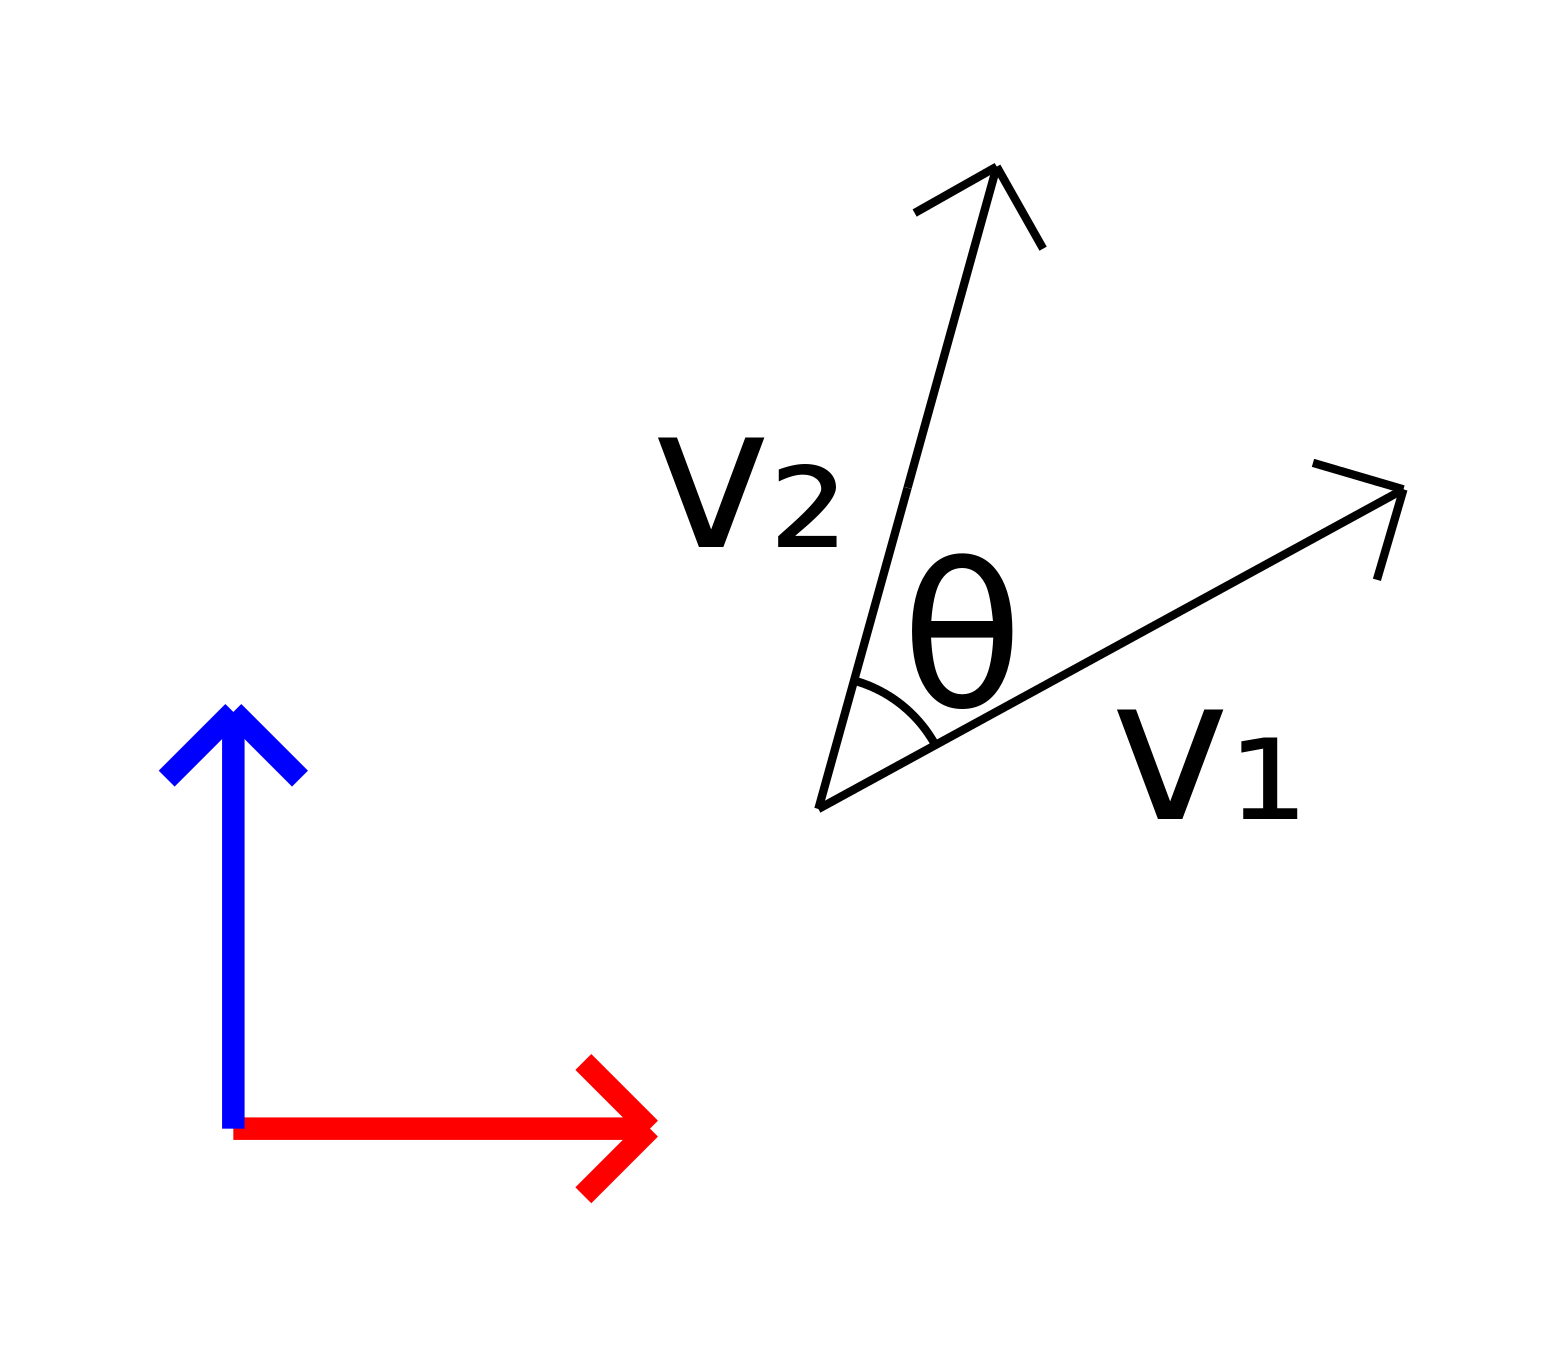
\includegraphics[scale=0.1]{generated_figures/bg_rotate_vec.png}
\hspace{1in}
% Drawing of frames i and j, where j is offset by \th
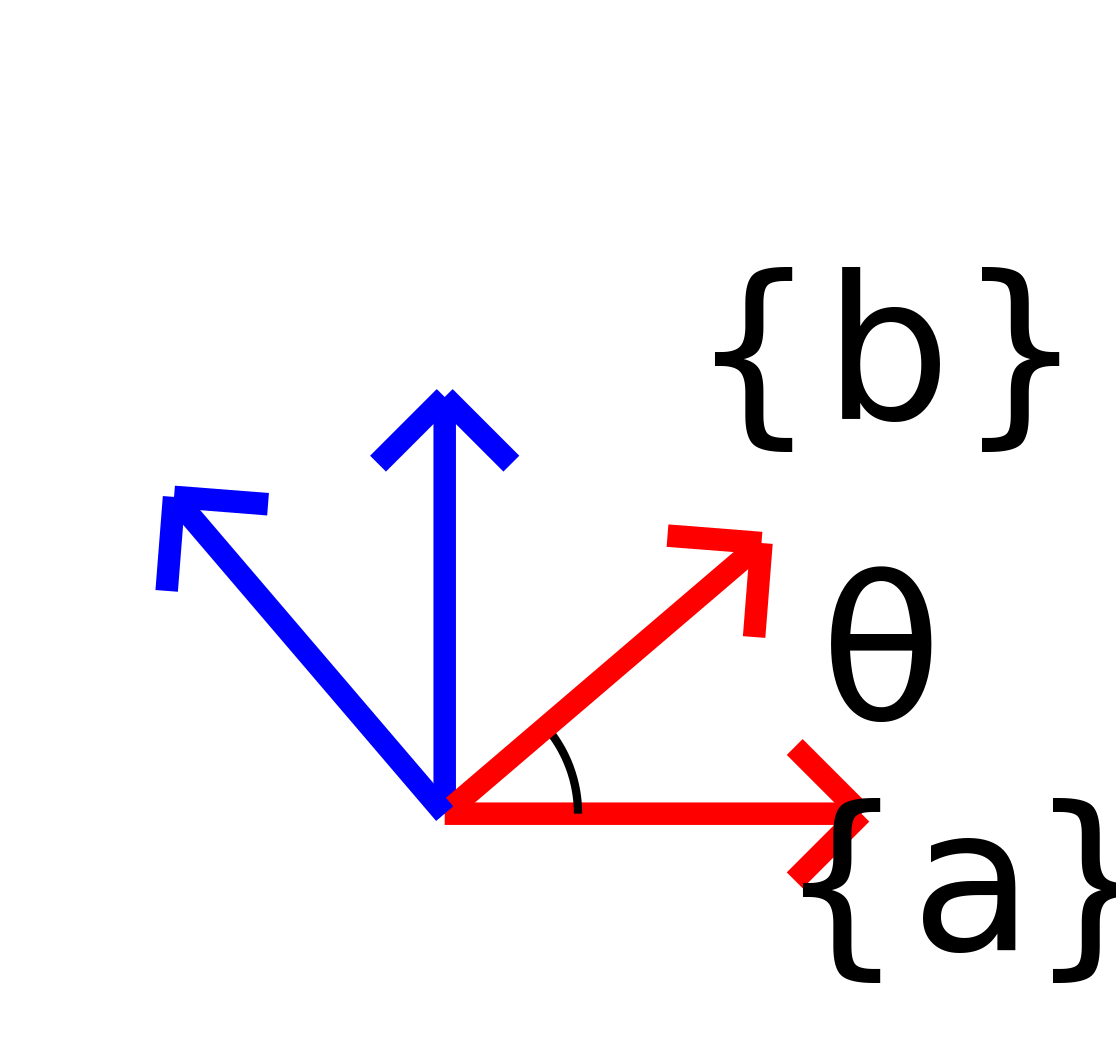
\includegraphics[scale=0.1]{generated_figures/bg_rotation.png}
\end{center}

A \emph{rotation matrix} \R{}{} represents rigid body rotations or rotational
offsets between coordinate frames.  In 2 dimensions, the rotation matrix
corresponding to a rotation of $\theta$ is
$$
\R{}{}(\theta) = \colvec{\cos(\theta)&-\sin(\theta)\\\sin(\theta)&\cos(\theta)}
$$

For rigid motions, this is the rotation of a body or vector by $\theta$; above
left, the vector $v_2 = \R{}{}(\theta) v_1$.

For transformations, \R{b}{a} is the rotation from \frame{a} to \frame{b} (above
right, $\R{b}{a} = \R{}{}(\theta)$). $\R{b}{a}$ can be described as:
\begin{itemize}
  \item The motion that rotates \frame{a} to \frame{b}.
  \item The representation of \frame{b} in \frame{a}; $\R{b}{a}$ can be found by
    expressing the axes of \frame{b} in \frame{a} as column vectors.
  \item The rotation that changes the representation of a vector $v$ from
    \frame{b} to \frame{a}: $\v{a} = \R{b}{a} \v{b}$.
\end{itemize}

\vspace{0.2in}
Furthermore, as shown in lecture, for any
rotation matrix \mat{R}, \inv{\mat{R}} = \trans{\mat{R}}.

\subsubsection{Compound Motions: Homogeneous Transforms}

Any rigid motion/transform between two frames can be expressed by combining a
single rotation and translation.  A \emph{homogeneous transform} is a single
matrix which allows us to express this combined rotation and translation:

$$
\H{b}{a} = \colvec{\R{b}{a}&\t{b}{a}\\0~0&1}
$$

As with previous notation, \H{b}{a} is a motion from \frame{a} to \frame{b}, or
equivalently the transform that changes the coordinates of points from \frame{b}
to \frame{a}.

% [ Drawing of frames i and j, where j is rotated by theta and offset by some
\begin{center}
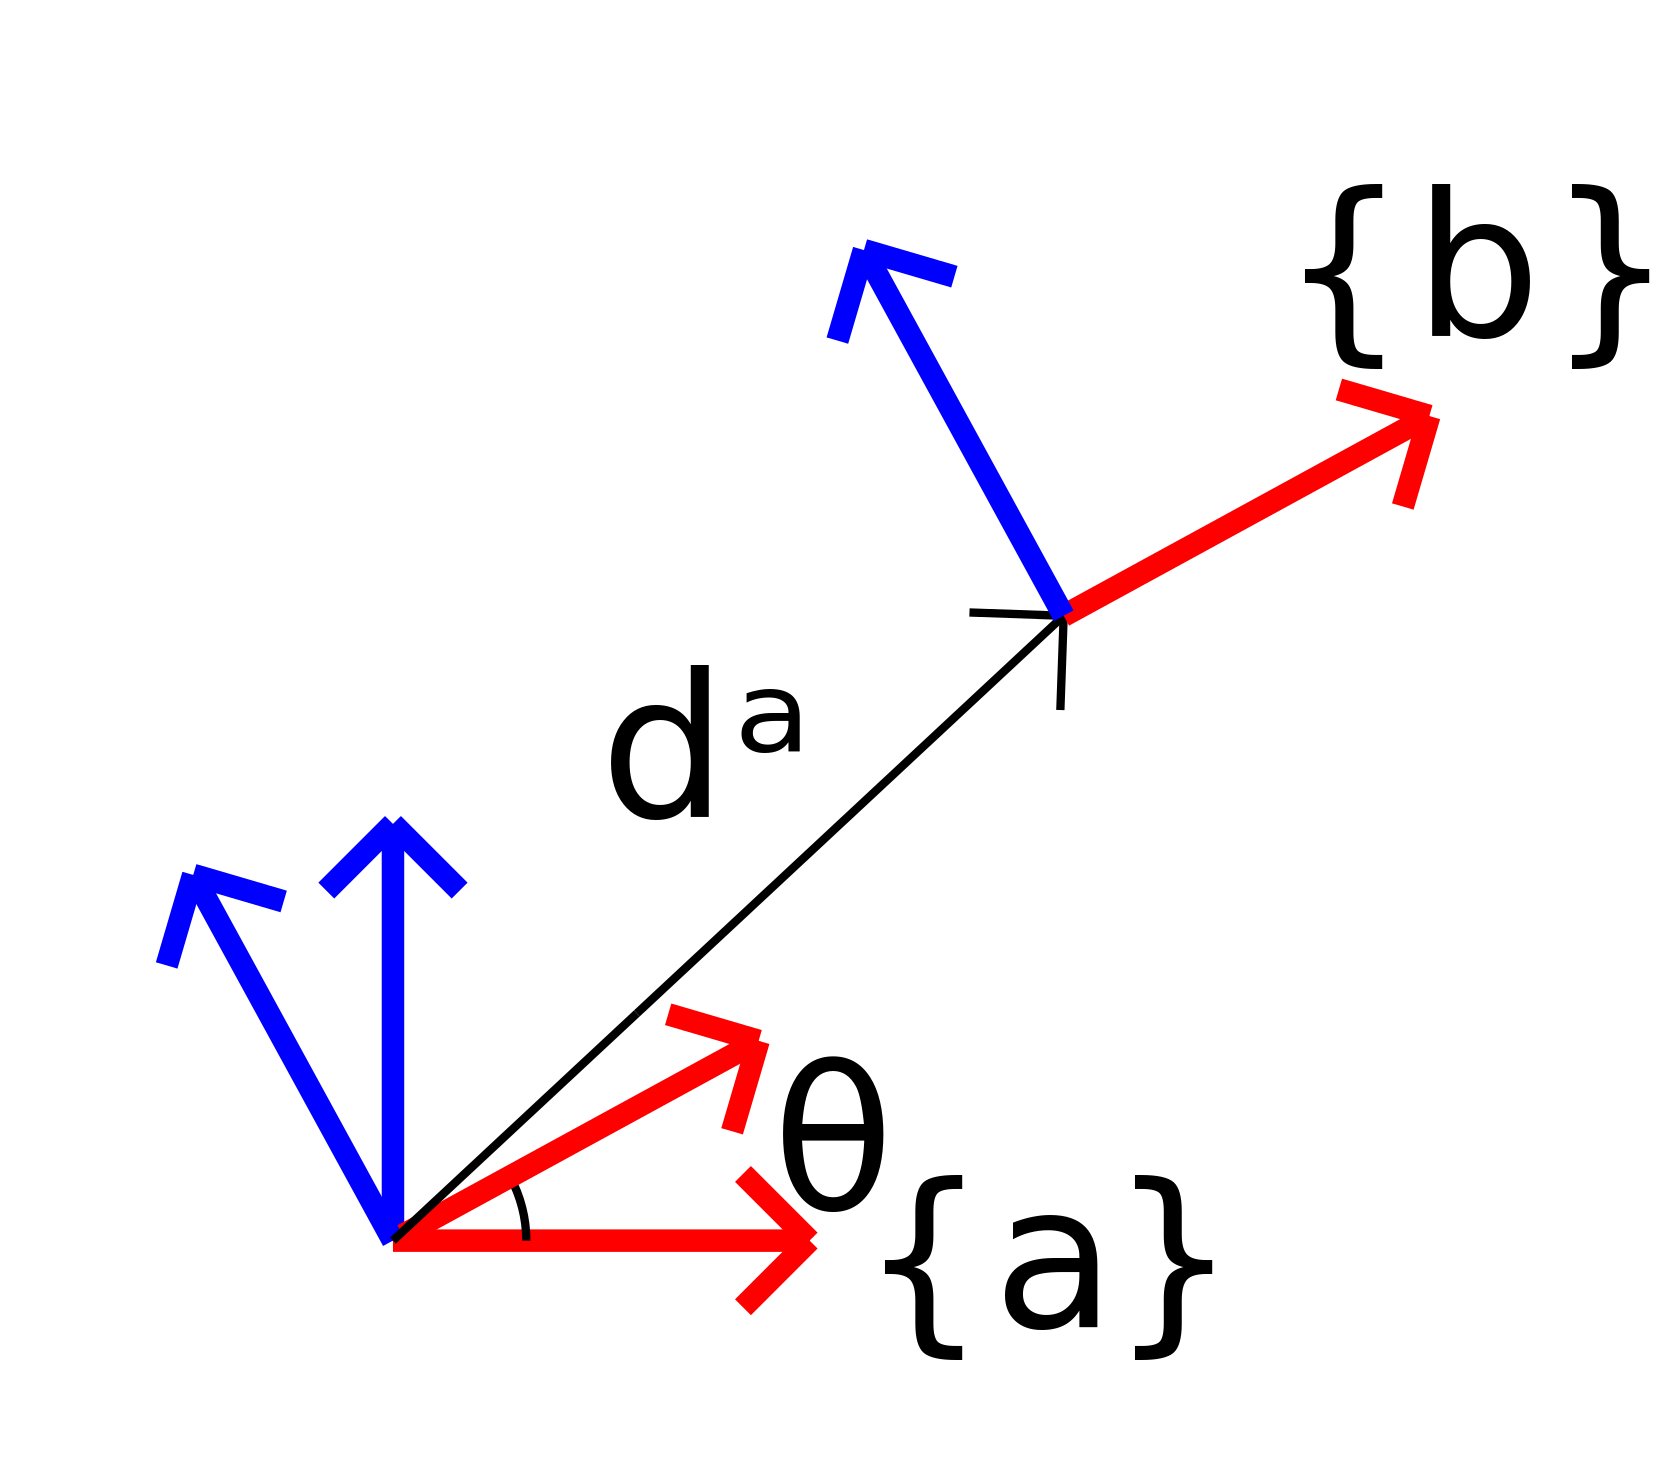
\includegraphics[scale=0.1]{generated_figures/bg_homo_r_then_t.png}
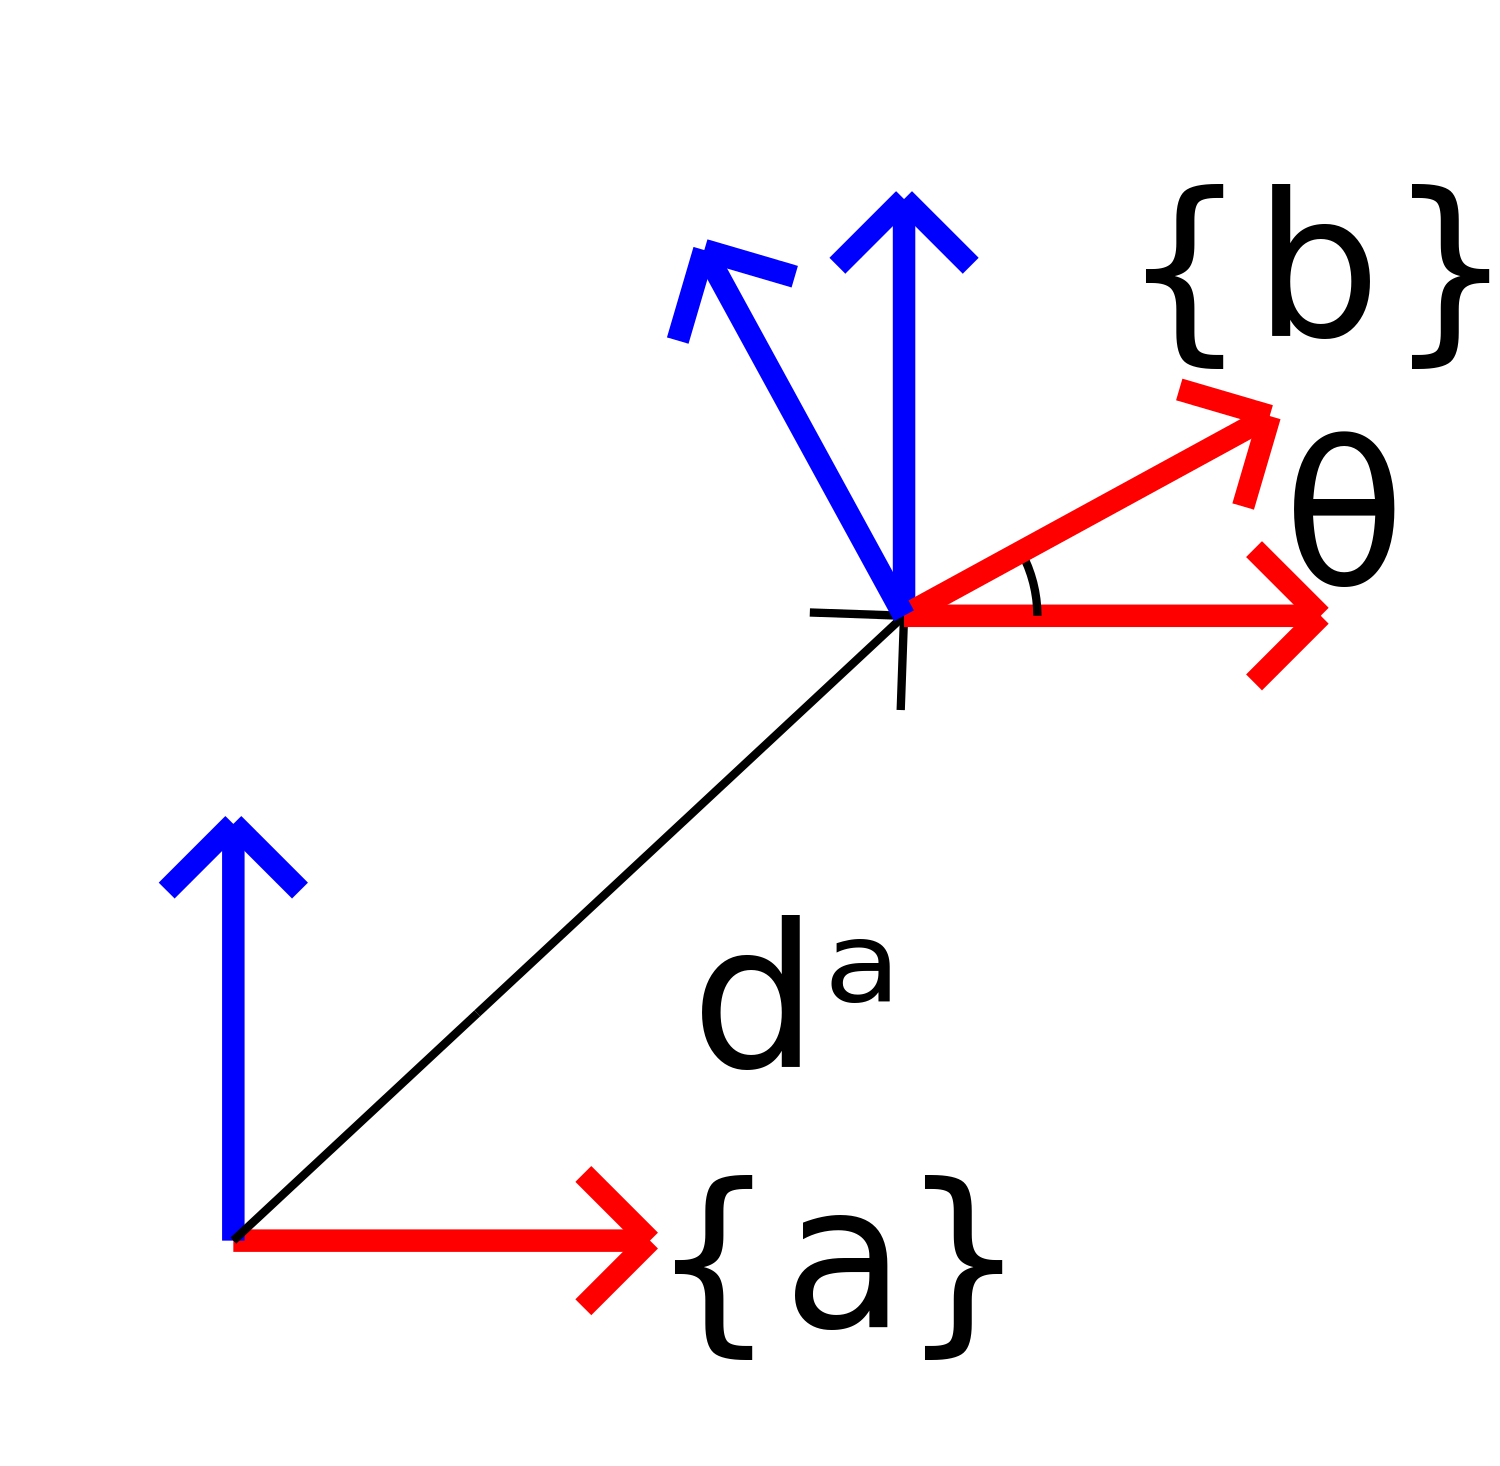
\includegraphics[scale=0.1]{generated_figures/bg_homo_t_then_r.png}
\end{center}

An important point here is that the \emph{order} and \emph{frame of reference}
which you apply the rotation and transforms here matter. The following two
descriptions are equivalent (and describe \H{b}{a}):
\begin{itemize}
\item First apply the rotation relative to \frame{a}, and then apply the
translation relative to \frame{a} (see above left).
\item First apply the translation relative to \frame{a} and then apply to
rotation relative to the \emph{new} frame resulting from this translation (see
above right).
\end{itemize}

Note that the other two potential descriptions - rotation then translation in
the new frame, or translation then rotation in \frame{a} - are both equivalent
but \textbf{do not describe \H{b}{a}}.

\subsubsection{Points, Vectors, and Homogeneous Transforms}

When using Homogeneous Transforms to operate on points and vectors, we must add
an extra coordinate to these values. Points are padded with a 1, so $\p{i} =
\smcolvec{p_x\\p_y}$ is now \smcolvec{p_x\\p_y\\1}, whereas vectors are padded with a 0,
so $\v{i} = \smcolvec{v_x\\v_y}$ is now \smcolvec{v_x\\v_y\\0}. This allows the
matrix dimensions to match when multiplying by such transforms.

If $\H{}{0}$ describes a motion in \frame{0}, then the point $\transform{q}{}{0}$
resulting from this motion starting at point $\p{0}$ is:

\begin{eqnarray*}
\transform{q}{}{0} &=& \H{}{0} \colvec{\p{0}\\1} \\
&=& \colvec{\R{}{0}&\t{}{0}\\0~0&1} \colvec{\p{0}\\1} \\
&=& \R{}{0} \p{0} + \t{}{0} \\
\end{eqnarray*}

Note that the $1$ we added to the bottom of the point results in the addition of
$\t{}{0}$; because free vectors have a $0$ added, they are only affected by the
rotation portion of \H{}{0}.

Using $\H{b}{a}$ as a transformation between coordinate representations of
points/vectors, we have

$$
\smcolvec{\p{a}\\1} = \H{b}{a} \smcolvec{\p{b}\\1} \text{and} \smcolvec{\v{a}\\0} = \H{b}{a} \smcolvec{\v{b}\\0}.
$$

\subsubsection{Inverting \H{b}{a}}
The inverse of \H{b}{a} is \H{a}{b}, representing the opposite motion, or a
reverse transform between the two frames.

To invert \H{b}{a}, we could perform the matrix inversion manually,
but there is a faster method using the properties of \H{b}{a}. First,
recall that \p{a} = \R{b}{a} \p{b} + \t{b}{a}.  Solving for \p{b}, we can see
that \p{b} = \trans{\R{b}{a}}\p{a} - \trans{\R{b}{a}}\t{b}{a}.  Therefore, given
\R{b}{a} and \t{b}{a}, \R{a}{b} = \trans{\R{b}{a}} and \t{a}{b} =
-\trans{\R{b}{a}}\t{b}{a}.  This finally gives us that

$$
\inv{\H{b}{a}} = \H{a}{b} = \smcolvec{\trans{\R{b}{a}}&(-\trans{\R{b}{a}}\t{b}{a})\\\trans{\vec{0}}&1}
$$

Inspection can show that this holds true for \v{a} and \v{b} as well.

\subsubsection{Composing Transforms}

Homogeneous transforms are composable. For example:
$$
\H{2}{0} = \H{1}{0} \H{2}{1}
$$

Note that in expressions like \p{1} = \H{0}{1}\p{0}, the superscripts ``cancel''
out, which gives you a quick check for your systems of equations.  However, note
that multiplication of transformations is \textbf{not} commutative and this
cancellation only works diagonally one way: $\H{2}{0} \ne \H{2}{1} \H{1}{0}$.
Using superscripts for the frame of points and vectors will help enforce this
consistency.

Furthermore, \inv{\H{i}{j}} = \H{j}{i}, so if we are given \H{1}{0}, \H{1}{2},
and \H{3}{2}, we can find \H{3}{0} = \H{1}{0}\inv{\H{1}{2}}\H{3}{2}.

\subsection{Forward Kinematics}

Forward kinematics is the idea of taking a robot's input parameters (joint
angles, link lengths, etc.) and finding the position of the end effector. We can do
this by writing homogeneous transforms that use the input parameters as
variables in order to find the final end effector position.  In effect, we want
to define frames at each link and joint and describe their differences in terms
of the robot parameters.

Let us consider the single link R arm of length $d$.
% DRAWING OF ARM
\begin{center}
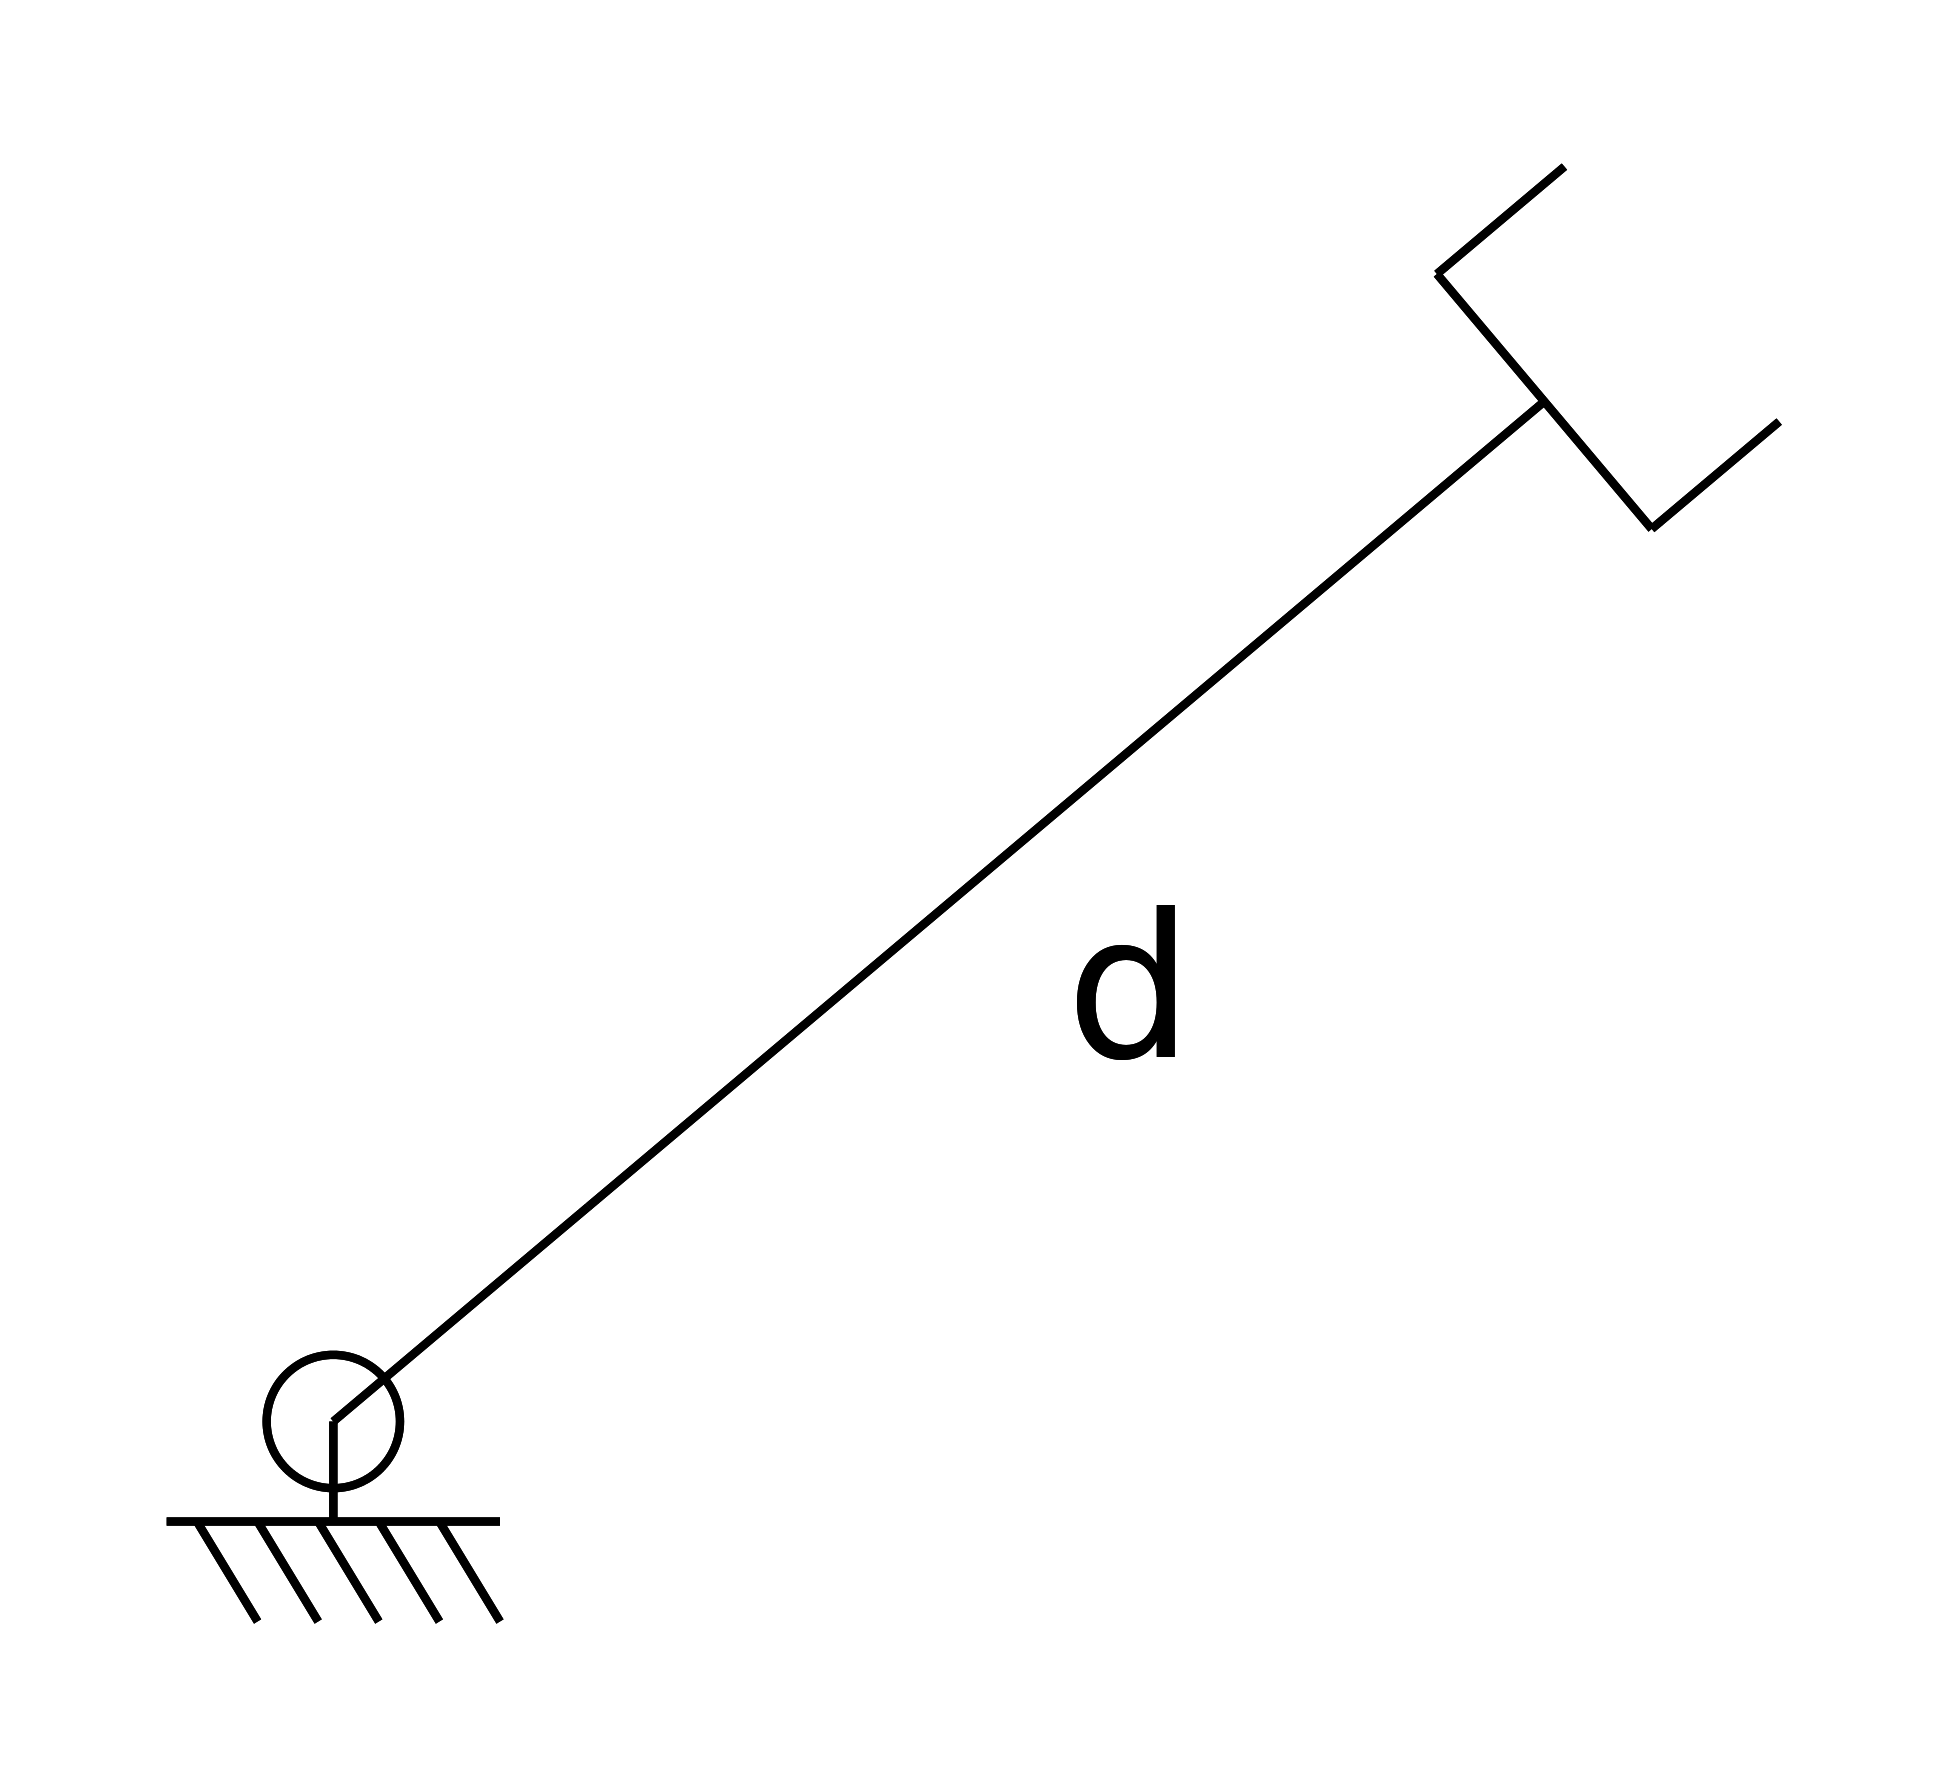
\includegraphics[scale=0.08]{generated_figures/bg_r_robot.png}
\end{center}

We wish to find the end effector position.  First, we can find it analytically
by noting that $x = d \cos(\th)$ and $y = d \sin(\th)$.  In vector form,
\smcolvec{x\\y} = \smcolvec{d \cos(\th)\\d\sin(\th)}.  While finding the forward
kinematics algebraically will always work, it definitely gets more error prone
with larger systems, and when composing multiple arms.  The way around this is using
homogeneous transforms.

We define one frame at the base, the base frame, usually labeled \vec{0}.
Let \frame{1} be another frame at the base of the link, but rotated by \th.
Finally, let \frame{2} be based at the end of the link, such that
$\transform{p}{e}{2} = \smcolvec{0\\0}$ in that frame is the end-effector position.

% [Drawing of said frames.]
\begin{center}
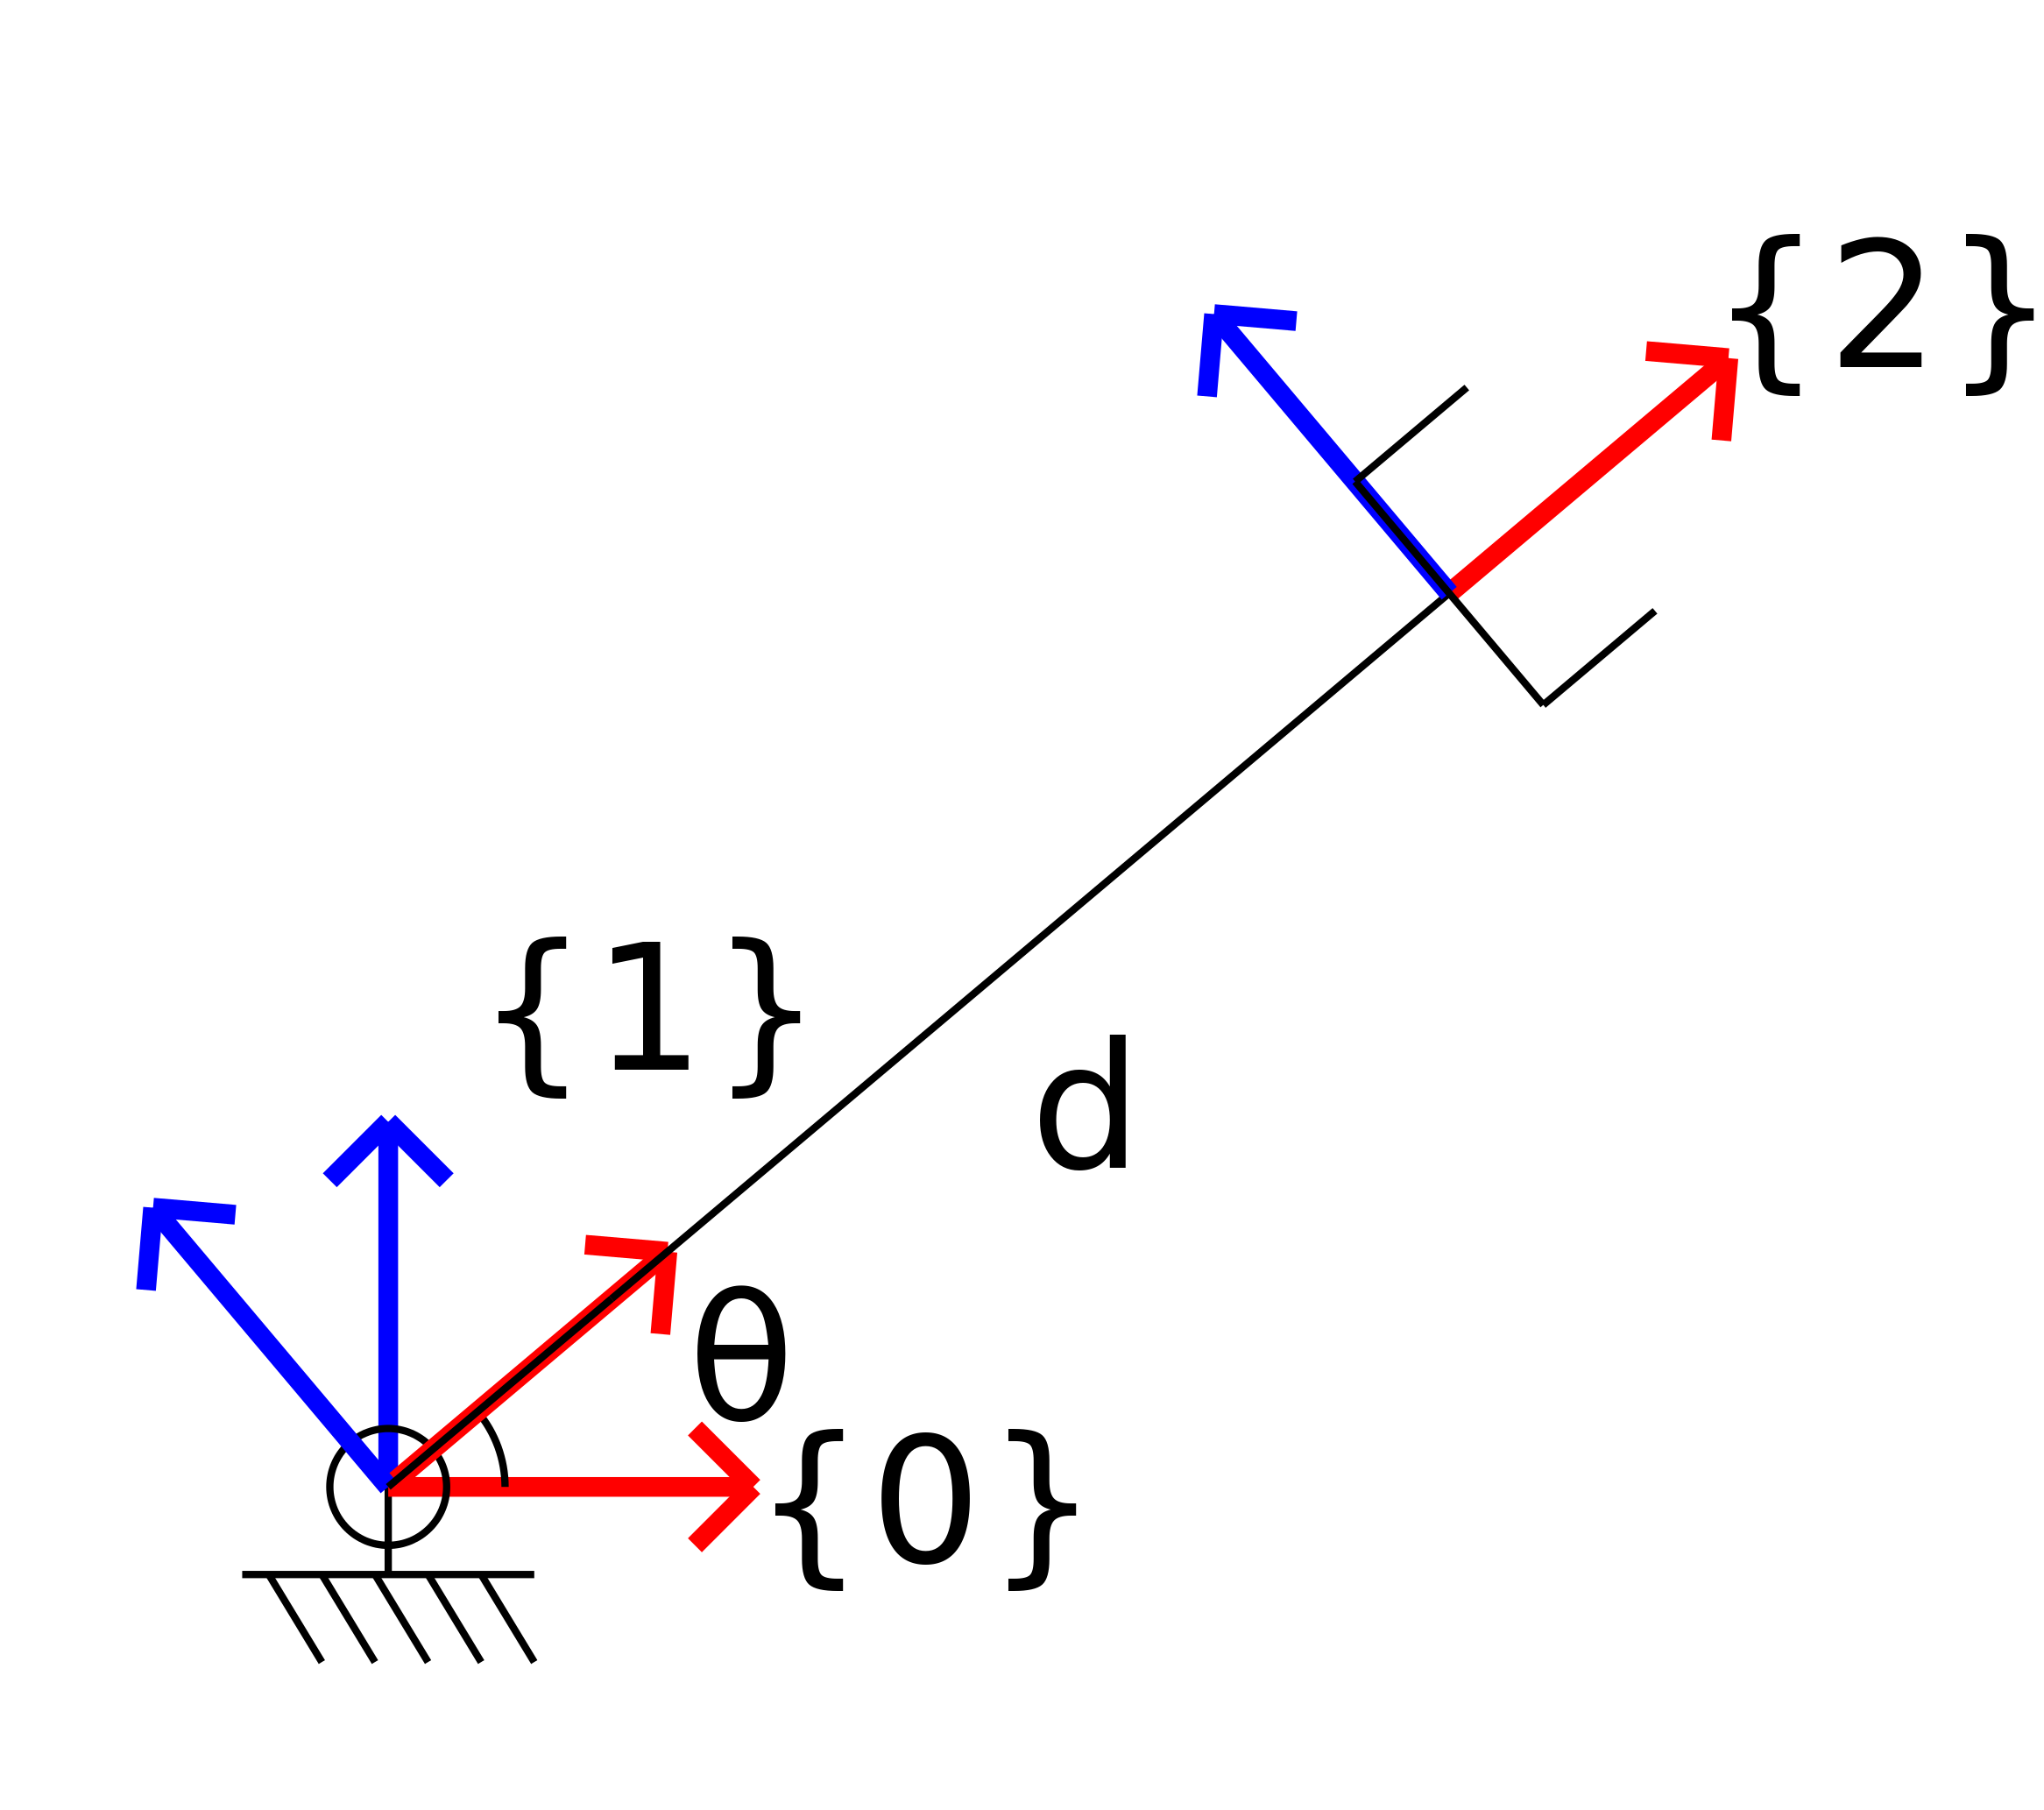
\includegraphics[scale=0.08]{generated_figures/bg_r_robot_frames.png}
\end{center}

Note that:

\begin{itemize}
    \item \H{1}{0} = \smcolvec{\mat{R_{\th}}&\vec{0}\\\trans{\vec{0}}&1} =
        \smcolvec{\cos(\th)&-\sin(\th)&0\\\sin(\th)&\cos(\th)&0\\0&0&1}
    \item \H{2}{1} = \smcolvec{1&0&d\\0&1&0\\0&0&1}
\end{itemize}

Therefore, \H{2}{0} = \H{1}{0}\H{2}{1} = \smcolvec{\cos(\th)&-\sin(\th)&d
\cos(\th)\\\sin(\th)&\cos(\th)&d\sin(\th)\\0&0&1}. Lastly, we can see that
$\H{2}{0} \transform{p}{e}{2} = \H{2}{0} \smcolvec{0\\0\\1} = \smcolvec{d \cos(\th)\\d \sin(\th)}$, which matches our analytical solution.

\section{In Class Questions}

    The following questions will be done in class, as a part of a group. Your group's answer will still need to be turned in with the rest of your assignment, however unlike the rest of the work this is allowed to be done in groups.
    
    \begin{questions}
    \titledquestion{Matrix Review}
    Given the Matrix
    $ A = \begin{bmatrix}
    -s_1- s_{12}& - s_{12} \\
    c_1 + c_{12}& c_{12}
    \end{bmatrix} $

    \begin{parts}
        \part[1] Is A an element of $SO(2)$?
        
        \begin{tcolorbox}[height=3cm]
         % TODO: ENTER YOUR ANSWER HERE
        \end{tcolorbox}
        
        \part[1] For what values of $\theta$ does rank(A) = 1?
        
        \begin{tcolorbox}[height=5cm]
         % TODO: ENTER YOUR ANSWER HERE
        \end{tcolorbox}
        
        \part[1] What is the inverse of A?
        
        \begin{tcolorbox}[height=5cm]
         % TODO: ENTER YOUR ANSWER HERE
        \end{tcolorbox}
        
        \newpage
        
        \part[1] Using (2) and (3), what values of $\theta$ can you not solve Ax = b, where x and b are column vectors?
        
        \begin{tcolorbox}[height=5cm]
         % TODO: ENTER YOUR ANSWER HERE
        \end{tcolorbox}
        
        \part[1] When rank(A)=1, what constraints are placed on b?
        
        \begin{tcolorbox}[height=5cm]
         % TODO: ENTER YOUR ANSWER HERE
        \end{tcolorbox}
    \end{parts}
    
    \titledquestion{Basic Transformations}
    Let \vec{t} = \smcolvec{-1\\1}, \th~=-\piover{4}

    \begin{parts}
        \part[1] Let \mat{H_1} be the homogeneous transformation that translates a
        point by \vec{t}. What is \mat{H_1}?
        
        \begin{tcolorbox}[height=5cm]
         % TODO: ENTER YOUR ANSWER HERE
        \end{tcolorbox}

        \newpage

        \part[1] Let \mat{H_2} be the homogeneous transformation that rotates a
        point by \th. What is \mat{H_2}?
        
        \begin{tcolorbox}[height=5cm]
         % TODO: ENTER YOUR ANSWER HERE
        \end{tcolorbox}
        
        \part[1] Show algebraically that \mat{H_1}\mat{H_2} is not equal to \mat{H_2}\mat{H_1}.
        
        \begin{tcolorbox}[height=15cm]
         % TODO: ENTER YOUR ANSWER HERE
        \end{tcolorbox}
        
        \newpage
        
        \part[1] Show geometrically that \mat{H_1}\mat{H_2} is not equal to \mat{H_2}\mat{H_1}.
        
        \begin{tcolorbox}[height=20cm]
         % TODO: ENTER YOUR ANSWER HERE
        \end{tcolorbox}
        
    \end{parts}
    
    \end{questions}

\writtenSection


\begin{questions}
    \titledquestion{Degrees of Freedom}
    How many degrees of freedom do each of these robots have (assume $\RR^2$)?
    

    \begin{parts}
        \part[1]
        \begin{align*}
        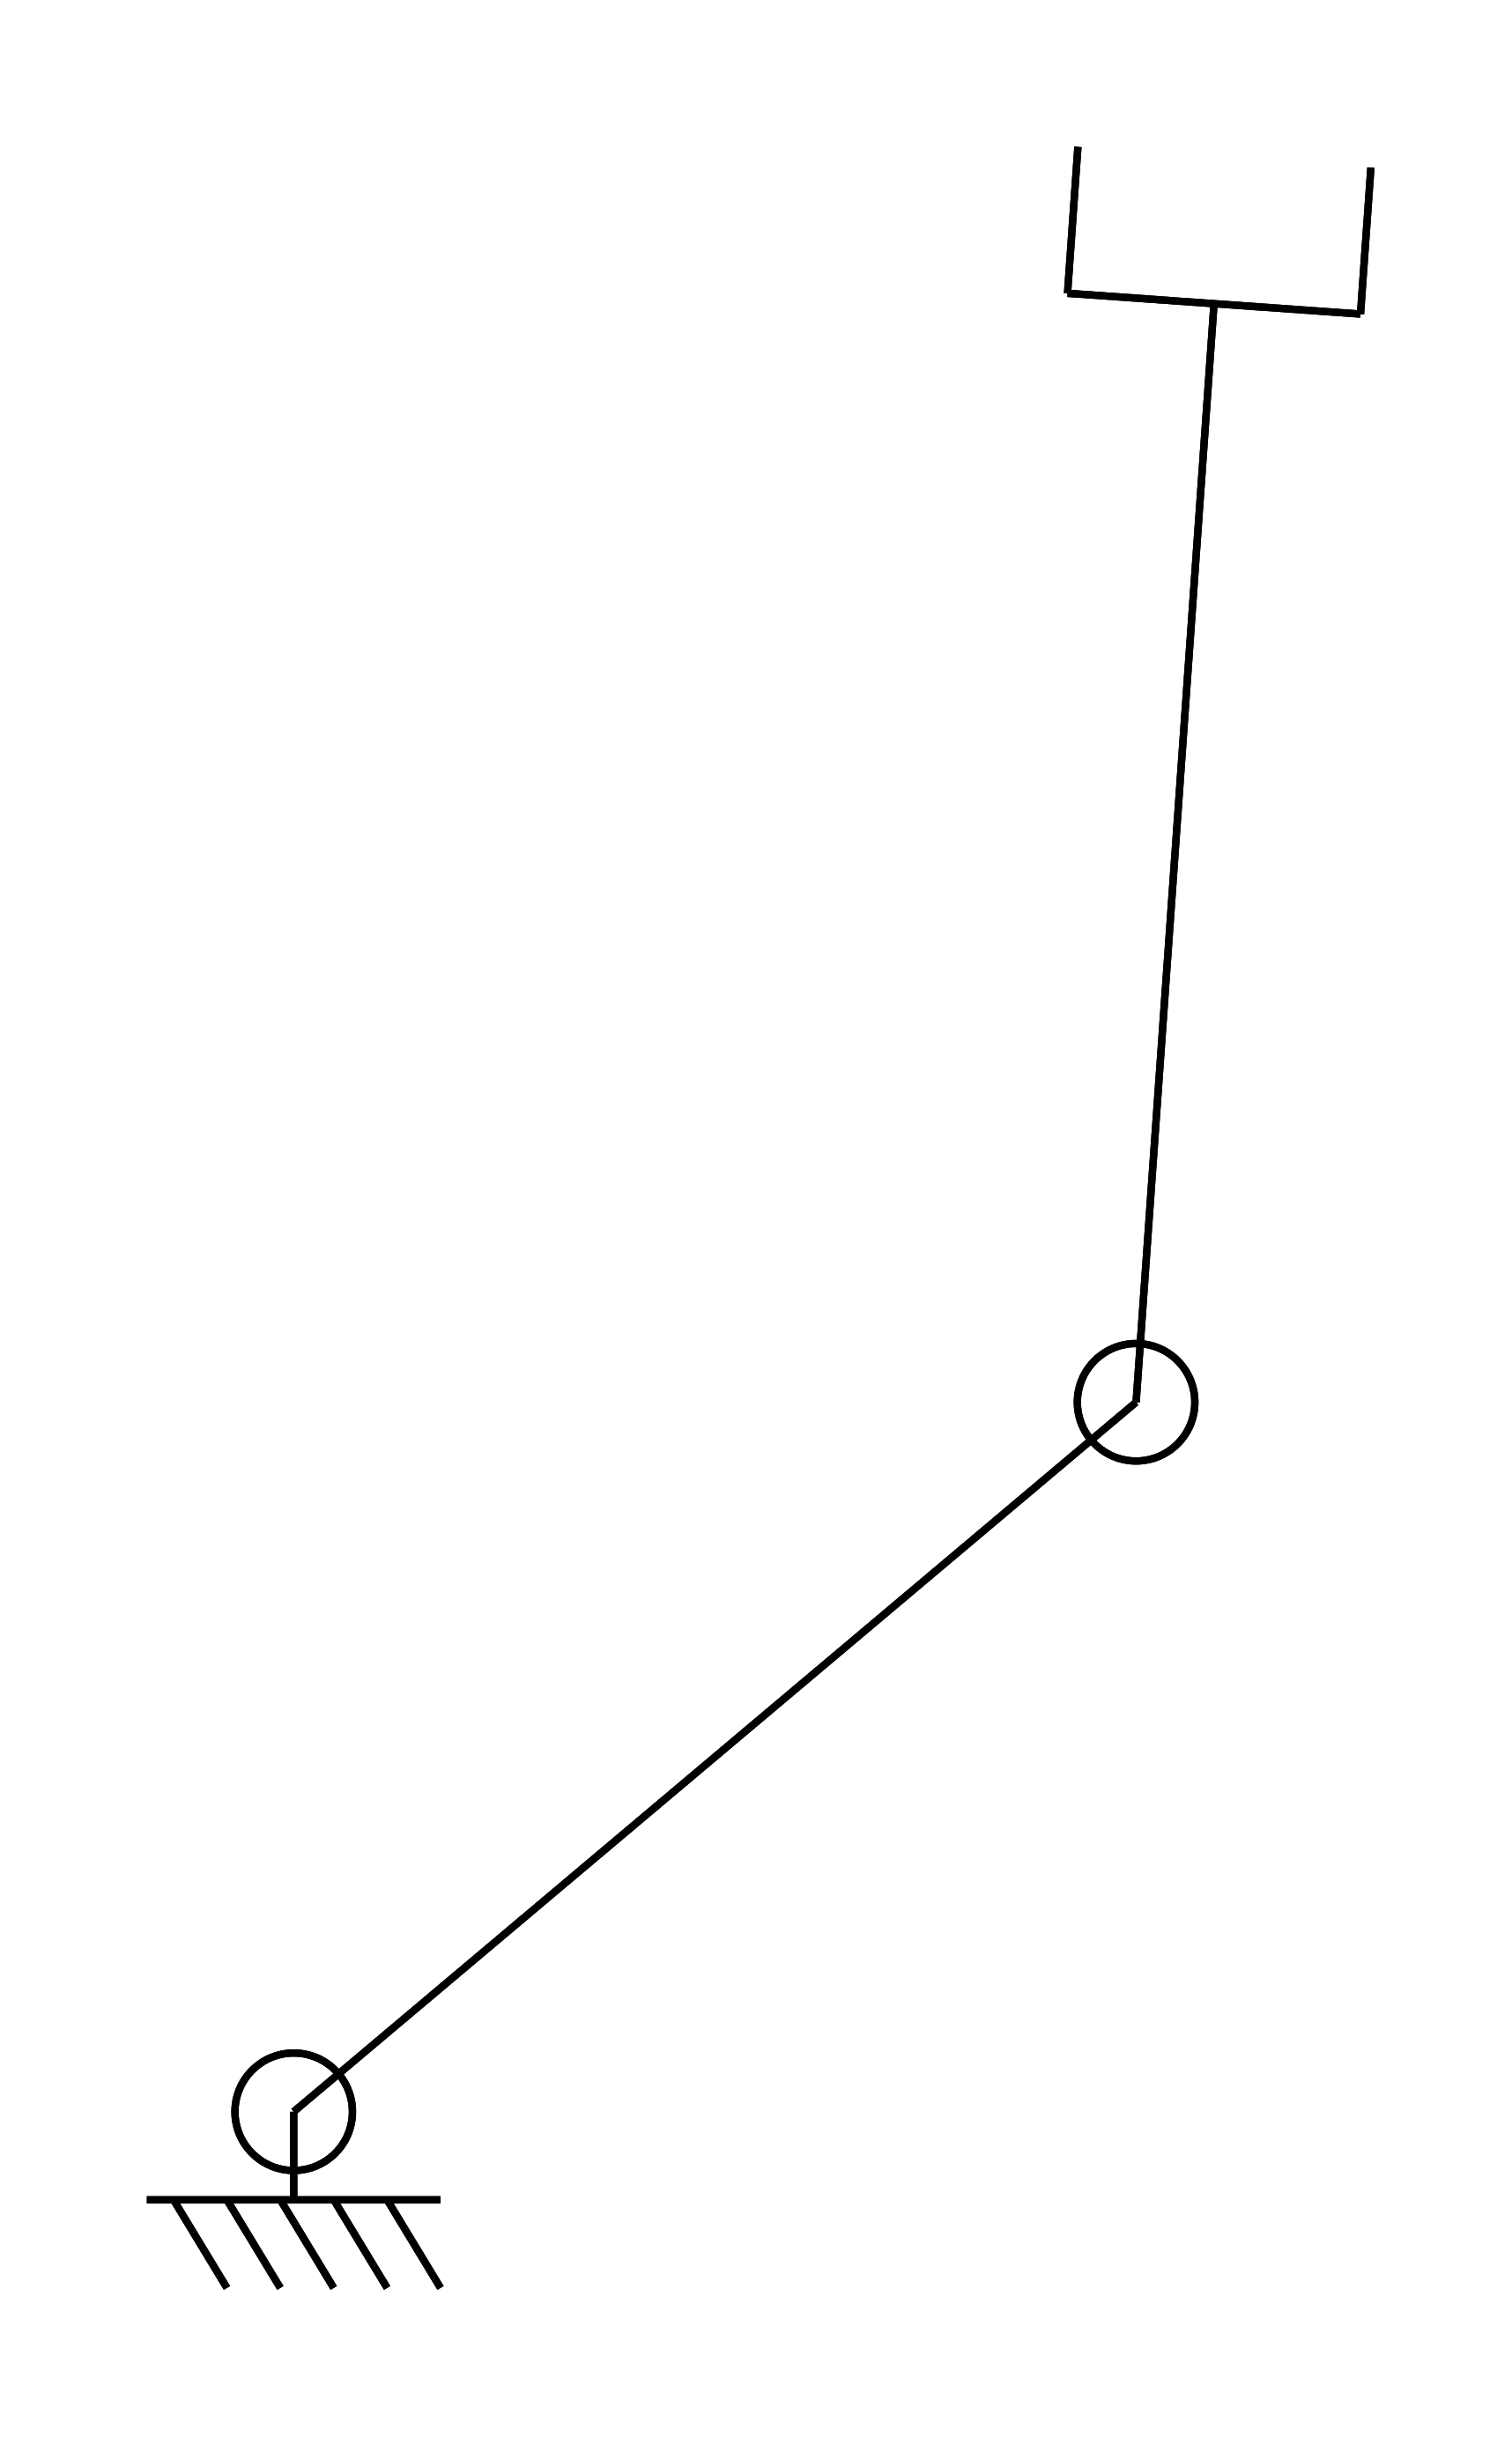
\includegraphics[scale=0.07]{generated_figures/robot_1a.png}
        \end{align*}
        
        \begin{tcolorbox}[height=3cm]
         % TODO: ENTER YOUR ANSWER HERE
        \end{tcolorbox}

        \part[1]
        \begin{align*}
        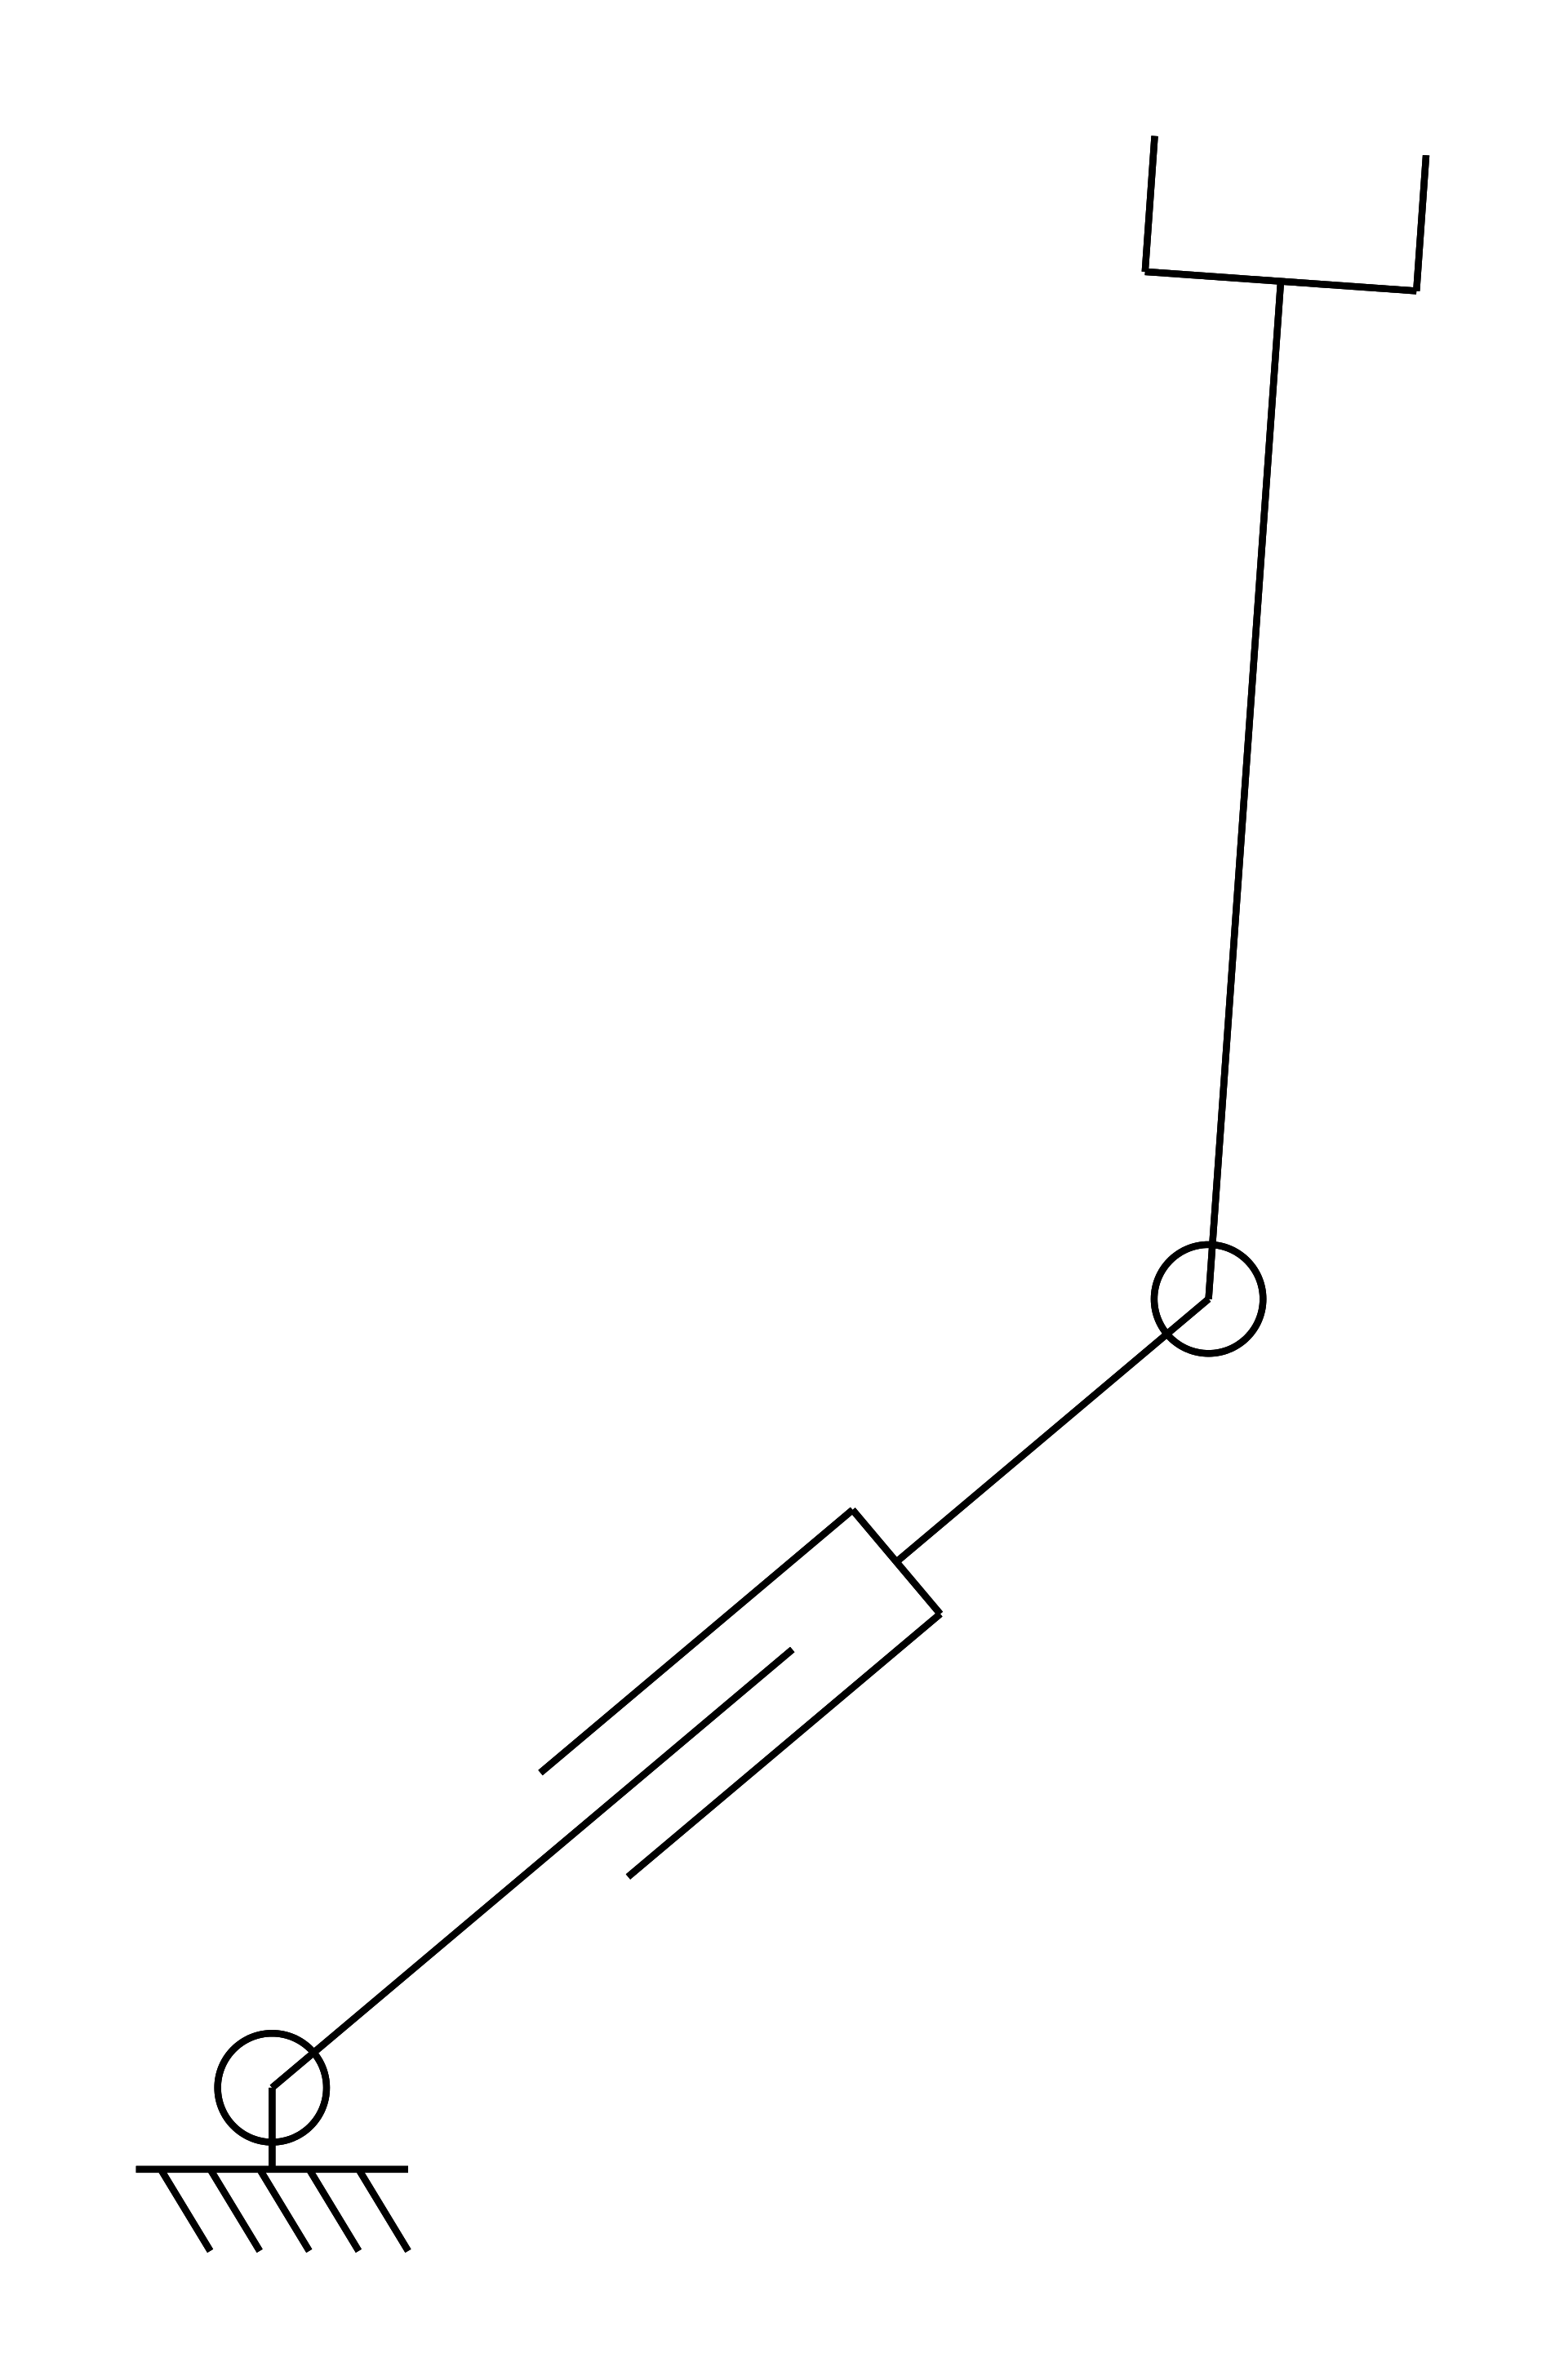
\includegraphics[scale=0.07]{generated_figures/robot_1b.png}
        \end{align*}
        
        \begin{tcolorbox}[height=3cm]
         % TODO: ENTER YOUR ANSWER HERE
        \end{tcolorbox}

        \part[1]
        \begin{align*}
        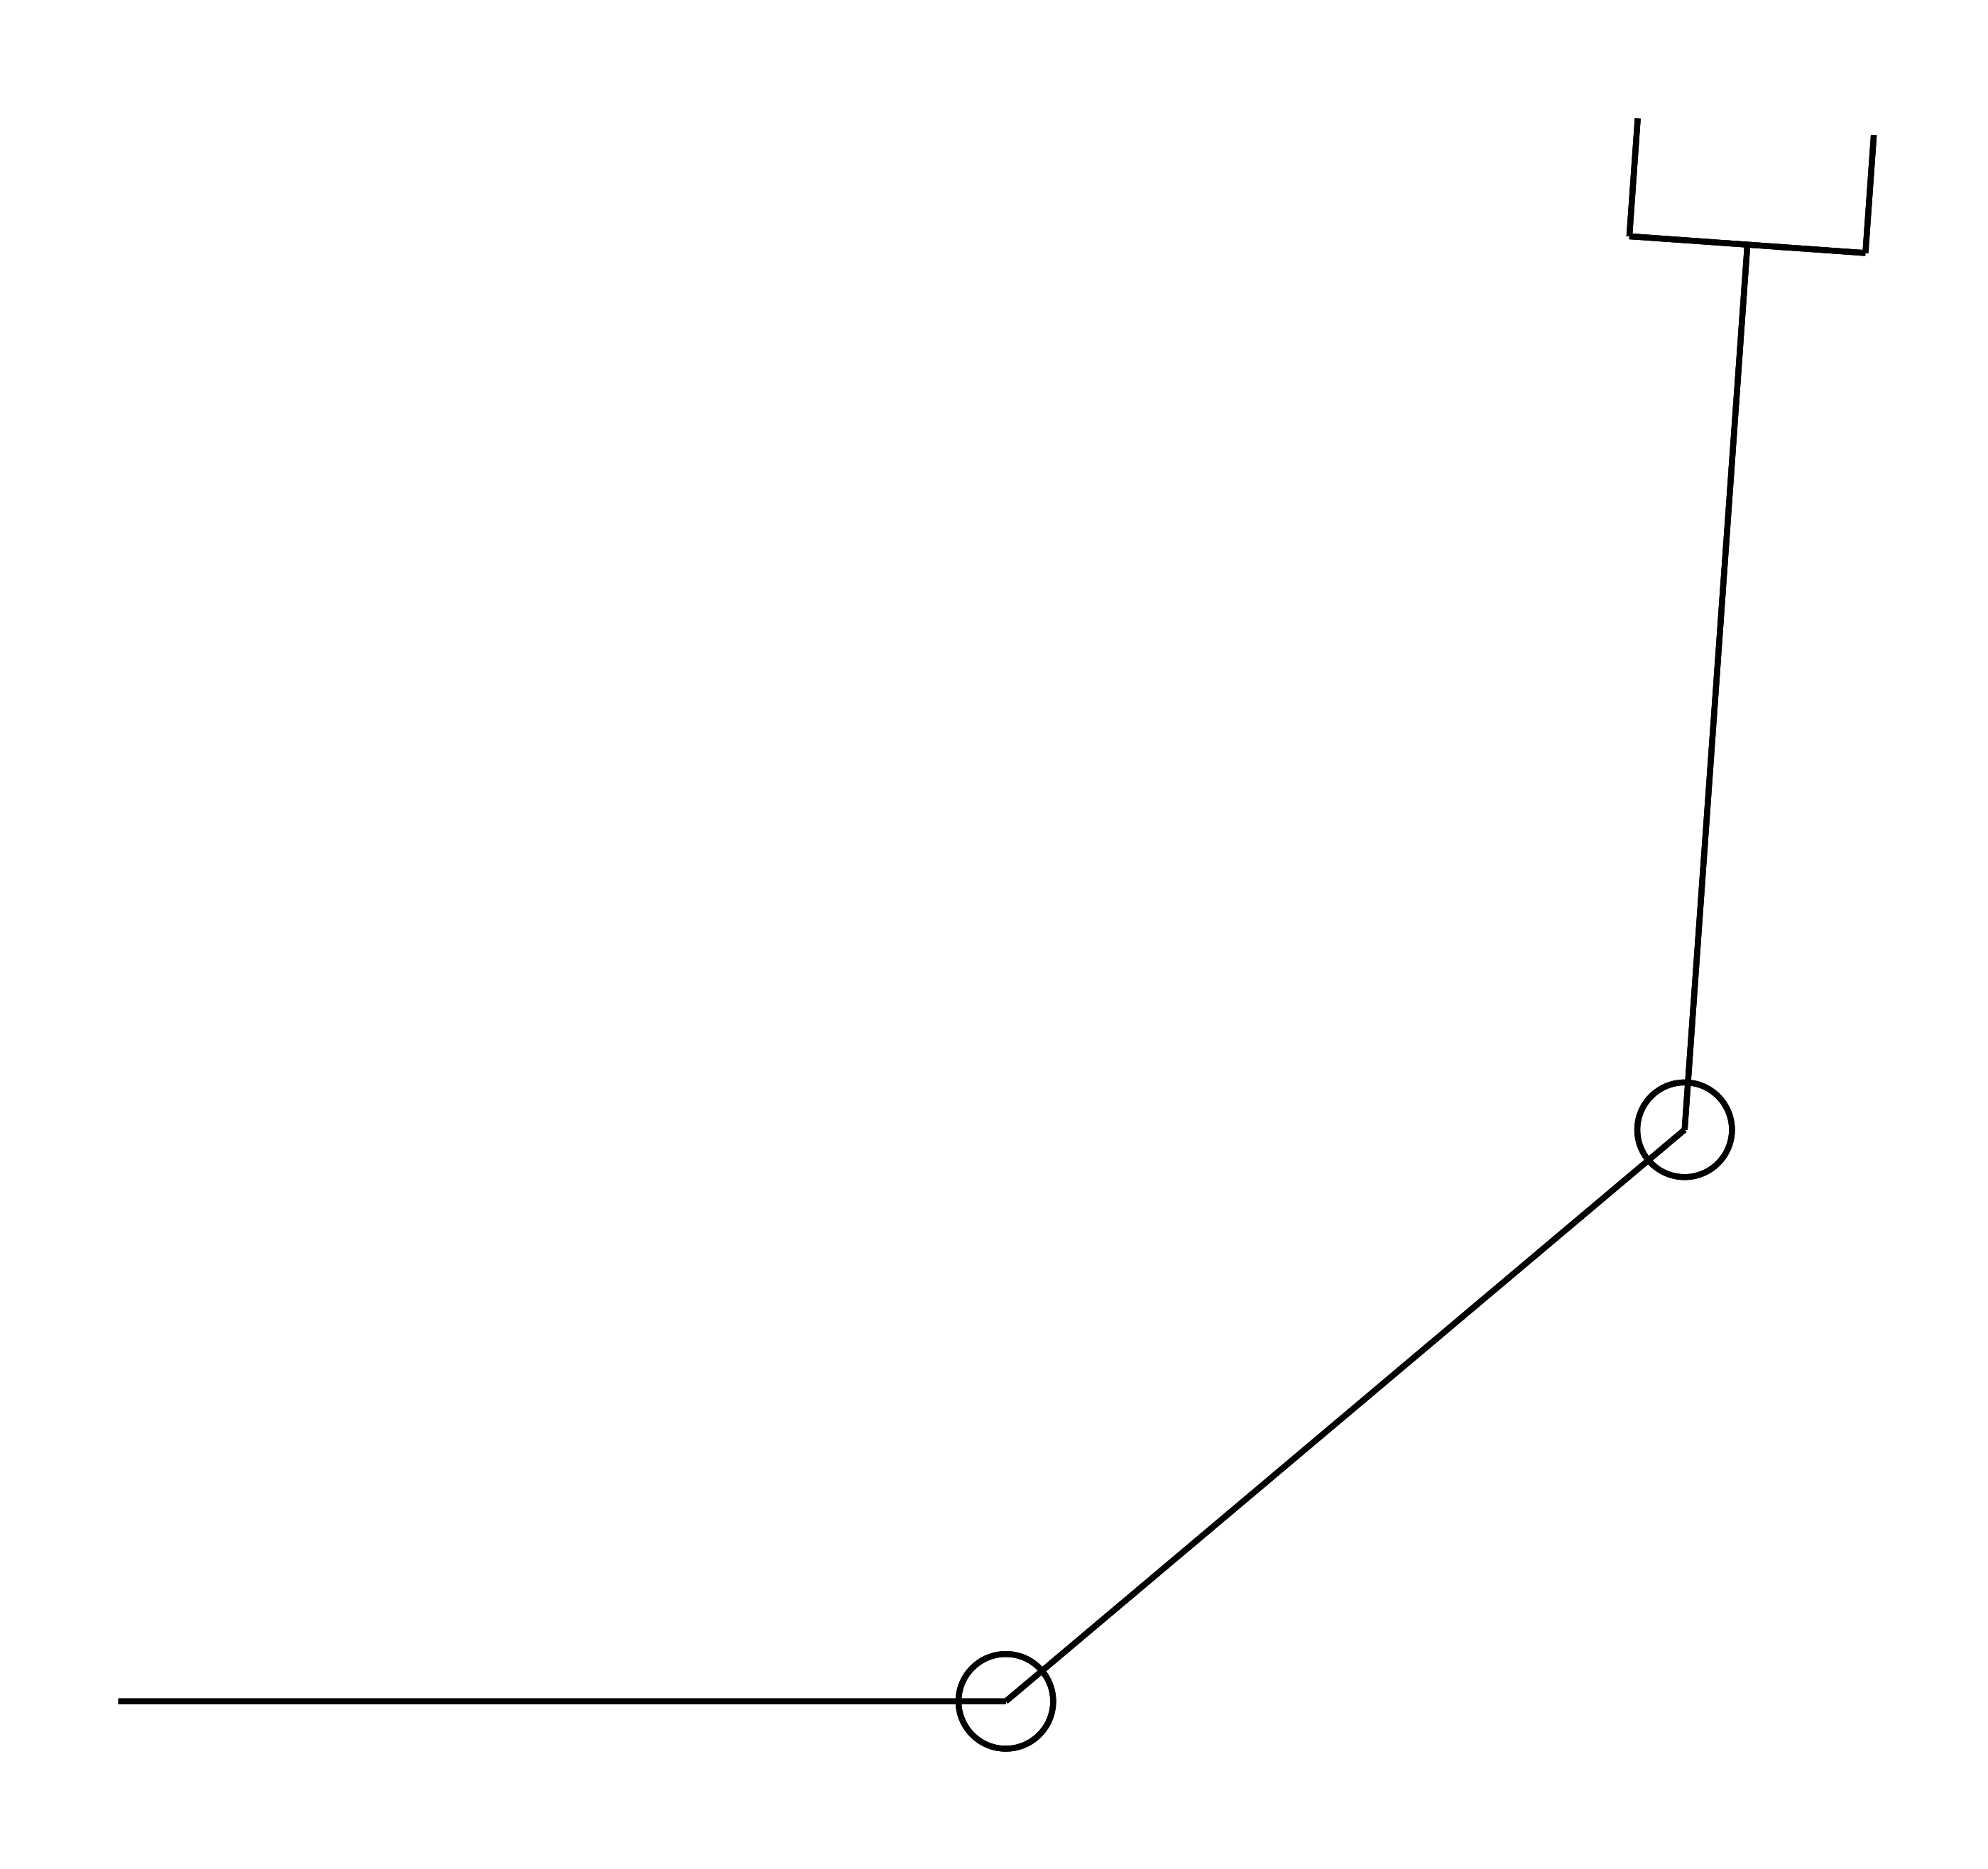
\includegraphics[scale=0.07]{generated_figures/robot_1c.png}
        \end{align*}
        
        \begin{tcolorbox}[height=3cm]
         % TODO: ENTER YOUR ANSWER HERE
        \end{tcolorbox}
        
        \part[1] 
        \begin{align*}
        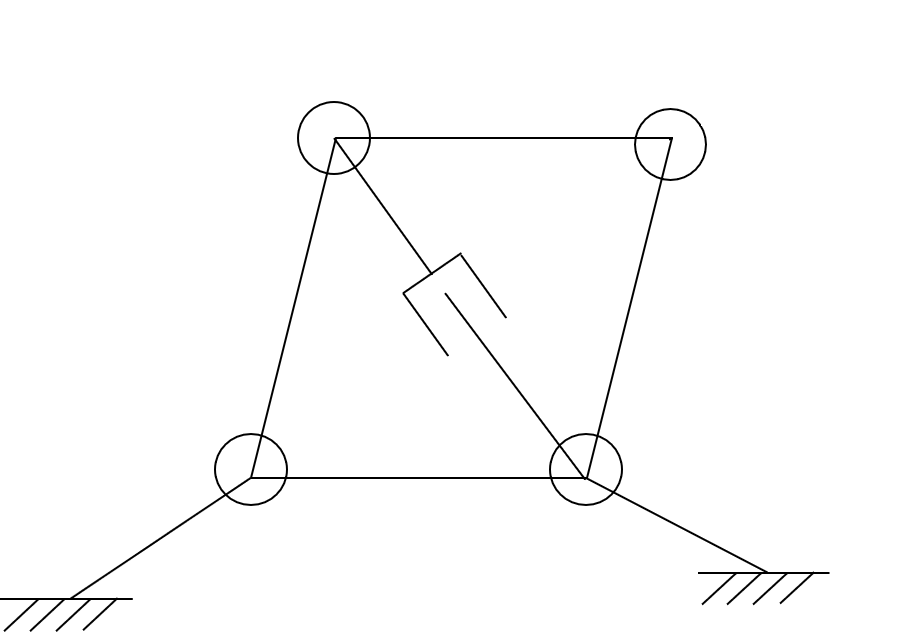
\includegraphics[scale=1]{generated_figures/robot_1d.png}
        \end{align*}
        
        \begin{tcolorbox}[height=3cm]
         % TODO: ENTER YOUR ANSWER HERE
        \end{tcolorbox}
        
    \end{parts}

    \newpage

    \titledquestion{Rotation Matrices}
    Let \vec{p} = \smcolvec{10\\0}.
    \begin{parts}

    \part[1] Let \mat{R} be the rotation matrix representing a rotation by \piover{4}.  Find \mat{R}.

    \begin{tcolorbox}[height=10cm]
     % TODO: ENTER YOUR ANSWER HERE
    \end{tcolorbox}

    \part[1] Let \vec{p'} be the result of applying \mat{R} to \vec{p}.  Find \vec{p'}.
    
    \begin{tcolorbox}[height=10cm]
     % TODO: ENTER YOUR ANSWER HERE
    \end{tcolorbox}

    \part[1] Draw and label a set of axes, \vec{p}, and \vec{p'} in this frame.

    \begin{tcolorbox}[height=20cm]
     % TODO: ENTER YOUR ANSWER HERE
    \end{tcolorbox}

    \end{parts}

    \newpage

    \titledquestion{Inverting Homogeneous Transformations}[5]
    Algebraically show that if \H{i}{j} =
    \smcolvec{\R{i}{j}&\t{i}{j}\\\trans{\vec{0}}&1}, then \inv{\H{i}{j}} =
    \smcolvec{\trans{\R{i}{j}}&-\trans{\R{i}{j}}\t{i}{j}\\\trans{\vec{0}}&1}.

    You do not need a formal proof, but you must show your steps clearly.

    \begin{tcolorbox}[height=20cm]
     % TODO: ENTER YOUR ANSWER HERE
    \end{tcolorbox}

    \newpage

    \titledquestion{Homogeneous Transformations}
    Let \vec{t} = \smcolvec{2\\5}, \th~=\piover{4}, and \frame{\alpha},
    \frame{\beta} be frames as shown in the following diagrams:

    \begin{center}
    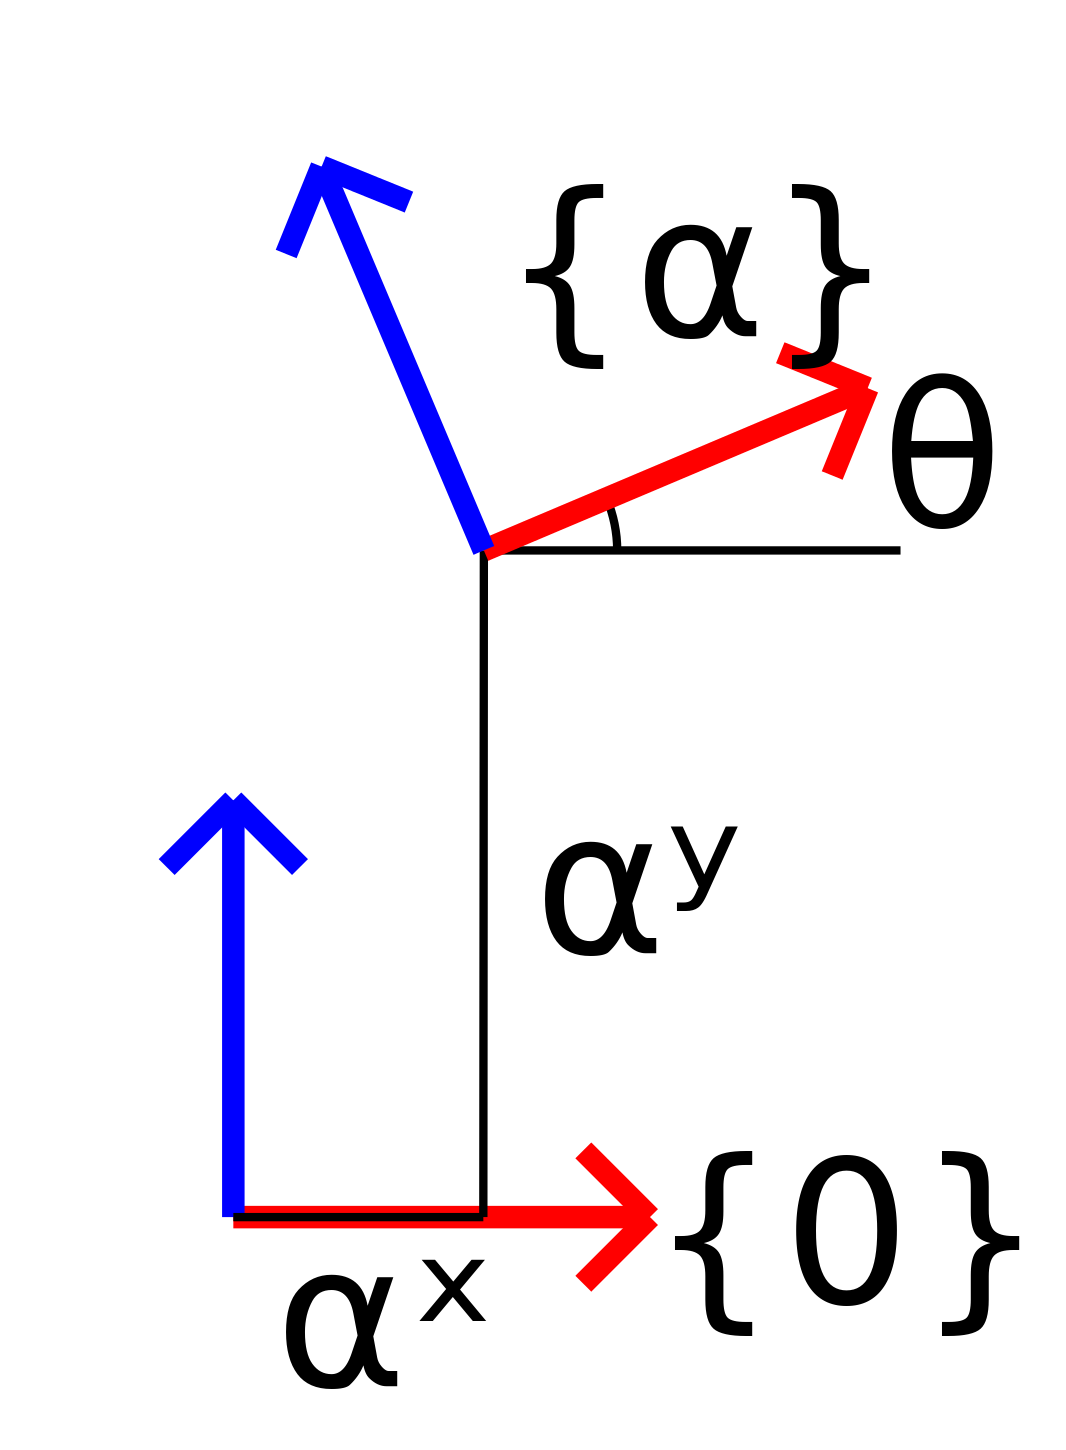
\includegraphics[scale=0.1]{generated_figures/frames_4c.png}
    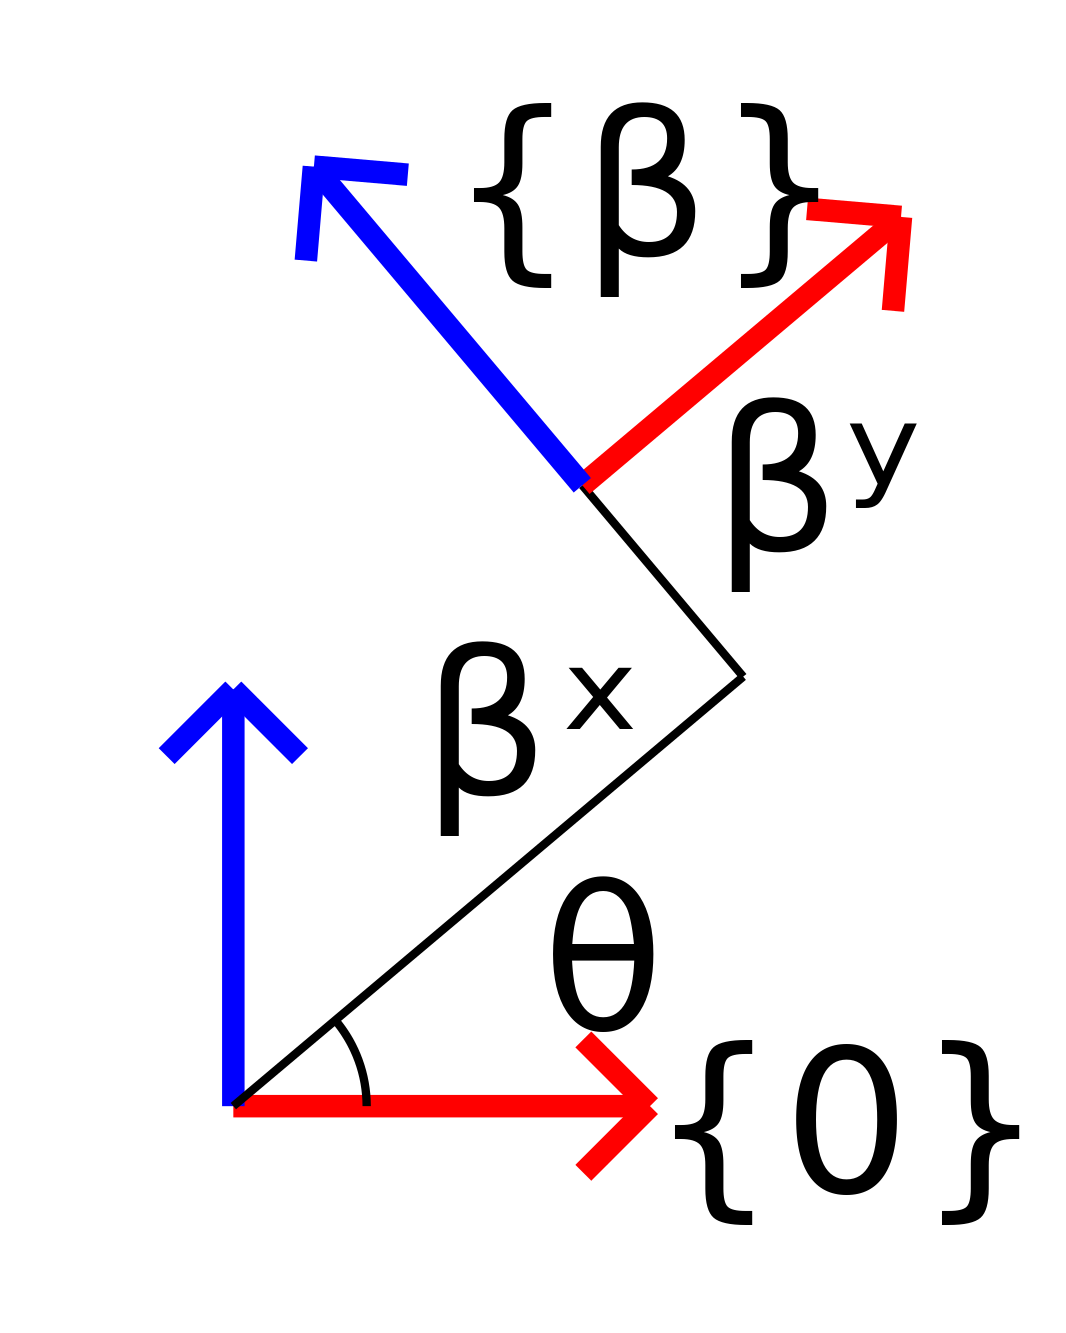
\includegraphics[scale=0.1]{generated_figures/frames_4d.png}
    \end{center}

    \begin{parts}
        \part[1] Let \mat{T_1} be the homogeneous transformation that translates a
        point by \vec{t}. What is \mat{T_1}?

        \begin{tcolorbox}[height=5cm]
         % TODO: ENTER YOUR ANSWER HERE
        \end{tcolorbox}

        \part[1] Let \mat{T_2} be the homogeneous transformation that rotates a
        point by \th. What is \mat{T_2}?
        
        \begin{tcolorbox}[height=8cm]
         % TODO: ENTER YOUR ANSWER HERE
        \end{tcolorbox}

        \part[5] Find \H{\alpha}{0}, using the frames shown in the figure.
        Verify your solution by using this matrix to transform the following
        points (given in \frame{\alpha}) to \frame{0}
        \begin{parts}
          \part \p{\alpha} = \smcolvec{0\\0}
          
          \begin{tcolorbox}[height=10cm]
           % TODO: ENTER YOUR ANSWER HERE
          \end{tcolorbox}
          
          \part \transform{q}{}{\alpha} = \smcolvec{1\\0}
          
          \begin{tcolorbox}[height=10cm]
           % TODO: ENTER YOUR ANSWER HERE
          \end{tcolorbox}
          
        \end{parts}
        and the following vectors (given in \frame{\alpha}) to \frame{0}.
        \begin{parts}
        \setcounter{partno}{2}
          \part \transform{v}{}{\alpha} = \smcolvec{0\\1}
          
          \begin{tcolorbox}[height=10cm]
           % TODO: ENTER YOUR ANSWER HERE
          \end{tcolorbox}
          
          \part \transform{u}{}{\alpha} = \smcolvec{1\\1}
          
          \begin{tcolorbox}[height=10cm]
           % TODO: ENTER YOUR ANSWER HERE
          \end{tcolorbox}
          
        \end{parts}
        \noindent Ensure that the coordinates make sense in the
        new representation.

        \setcounter{partno}{3}

        \part[5] Find \H{\beta}{0}, using the frames shown in the figure.
        Verify your solution by using this matrix to transform the following
        points (given in \frame{\beta})  to \frame{0}
        \begin{parts}
          \part \p{\beta} = \smcolvec{0\\0}
          
          \begin{tcolorbox}[height=10cm]
           % TODO: ENTER YOUR ANSWER HERE
          \end{tcolorbox}
          
          \part \transform{q}{}{\beta} = \smcolvec{1\\0}
          
          \begin{tcolorbox}[height=10cm]
           % TODO: ENTER YOUR ANSWER HERE
          \end{tcolorbox}
          
        \end{parts}
        \noindent and the following vectors (given in \frame{\beta}) to \frame{0}. 
       	\begin{parts}
        	\setcounter{partno}{2} 
          	\part \transform{v}{}{\beta} = \smcolvec{0\\1}
          	
          	\begin{tcolorbox}[height=10cm]
             % TODO: ENTER YOUR ANSWER HERE
            \end{tcolorbox}
          	
          	\part \transform{u}{}{\beta} = \smcolvec{1\\1}
          	
          	\begin{tcolorbox}[height=10cm]
             % TODO: ENTER YOUR ANSWER HERE
            \end{tcolorbox}
        \end{parts}
        \noindent Ensure that the coordinates make sense in the
        new representation.

        \part[1] Find \H{\beta}{\alpha}.

        \begin{tcolorbox}[height=20cm]
           % TODO: ENTER YOUR ANSWER HERE
        \end{tcolorbox}

        \newpage

        \part[2] Compute \H{\alpha}{0} and \inv{\H{\alpha}{0}}. Verify that
        (\inv{\H{\alpha}{0}} \H{\alpha}{0}) = \smcolvec{1&0&0\\0&1&0\\0&0&1}.
        
        \begin{tcolorbox}[height=20cm]
           % TODO: ENTER YOUR ANSWER HERE
        \end{tcolorbox}
        
    \end{parts}

    \newpage

    \titledquestion{Workspace and Frames}
    Consider the following robot:

    \begin{center}
    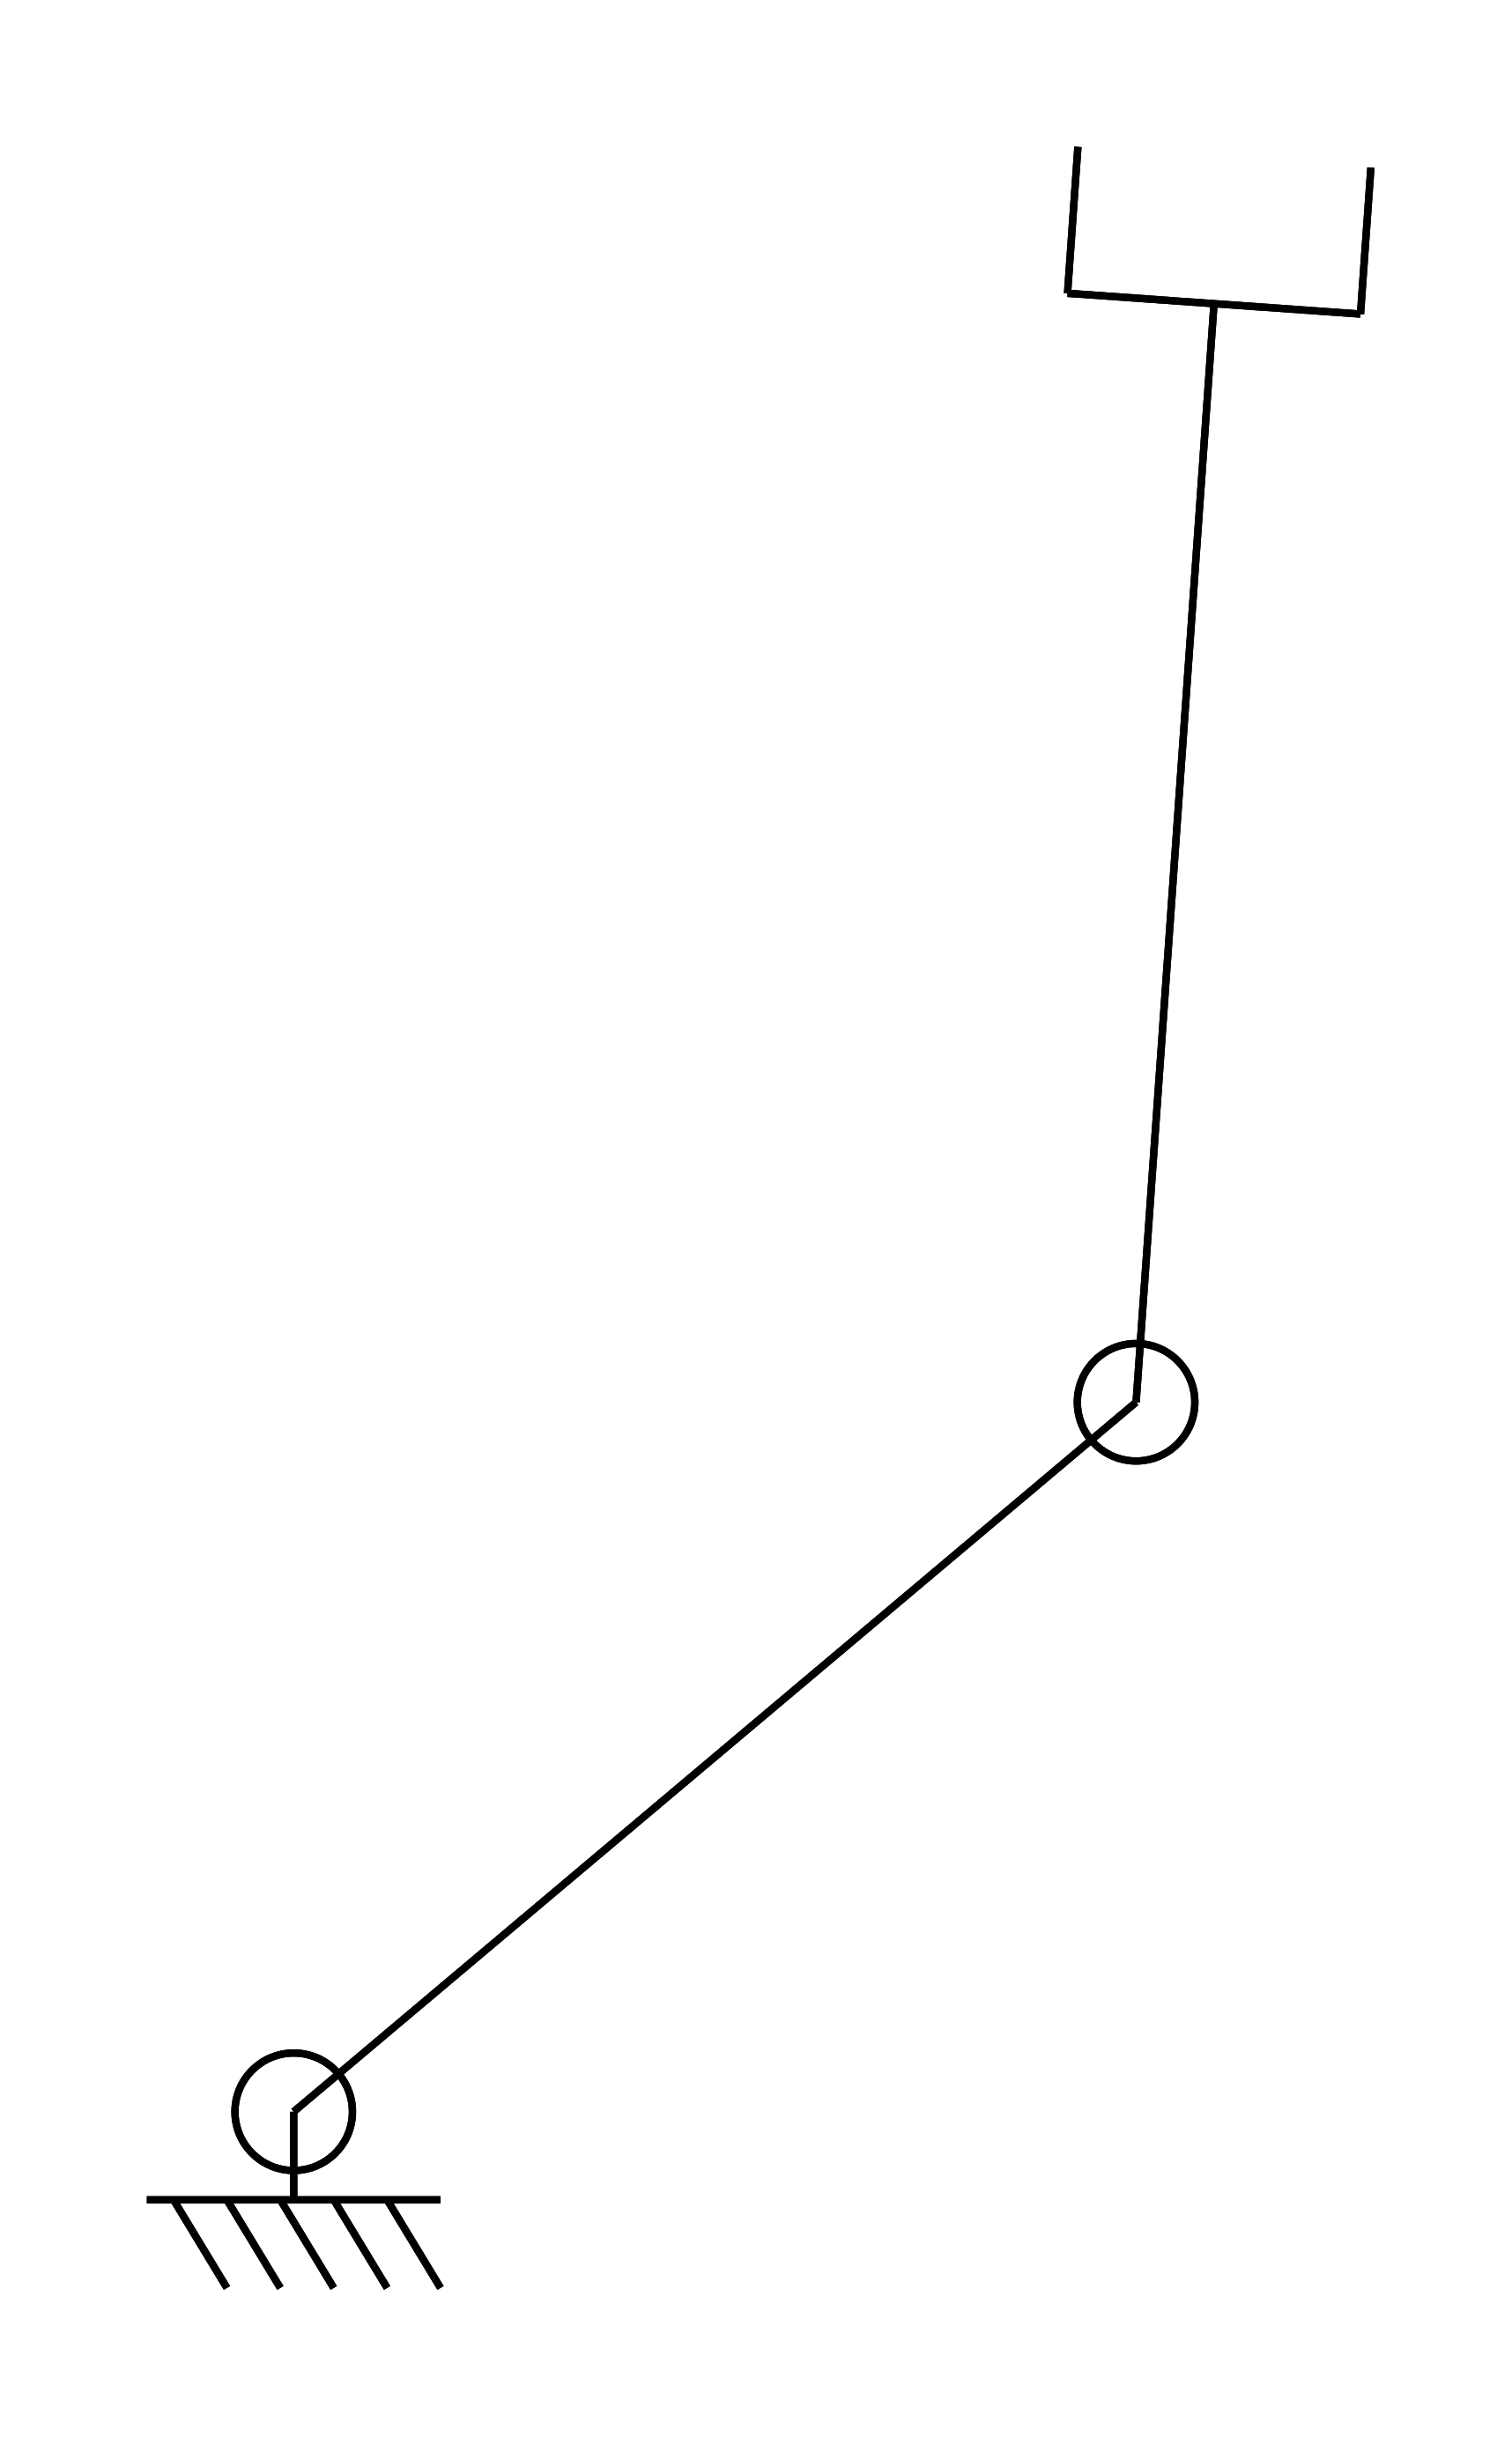
\includegraphics[width=1.5in]{generated_figures/robot_5.png}
    \end{center}

    Draw and clearly label the following, \textbf{using the frame conventions given in
    the background for this assignment}.
    \begin{parts}
        \part[1] The base frame of the entire robot: \frame{0}.
        \part[1] The starting frame for the first link: \frame{1}
        \part[1] The frame at the end of the first link: \frame{2}
        \part[1] The starting frame for the second link: \frame{3}
        \part[1] The end effector frame: \frame{4}
        
        \newpage
        
        \begin{tcolorbox}[height=20cm]
           % TODO: ENTER YOUR ANSWER HERE
        \end{tcolorbox}
        
        \newpage
        
        \part[3] Assume $l_1 > l_2$. On a separate plot, shade the workspace (in
        $\RR^2$), ignoring self-collision. Label the dimensions of this plot.
        
        \begin{tcolorbox}[height=20cm]
           % TODO: ENTER YOUR ANSWER HERE
        \end{tcolorbox}
        
    \end{parts}

    \newpage

    \titledquestion{Forward Kinematics of an RR Arm}
    For the robot in the previous question, compute the following in terms of
    $l_1$, $l_2$, $\th[1]$, and $\th[2]$:

    \begin{parts}
        \part[1] \H{1}{0}
        
        \begin{tcolorbox}[height=10cm]
           % TODO: ENTER YOUR ANSWER HERE
        \end{tcolorbox}
        
        \part[1] \H{2}{1}
        
        \begin{tcolorbox}[height=10cm]
           % TODO: ENTER YOUR ANSWER HERE
        \end{tcolorbox}
        
        \newpage
        
        \part[1] \H{3}{2}
        
        \begin{tcolorbox}[height=10cm]
           % TODO: ENTER YOUR ANSWER HERE
        \end{tcolorbox}
        
        \part[1] \H{4}{3}
        
        \begin{tcolorbox}[height=10cm]
           % TODO: ENTER YOUR ANSWER HERE
        \end{tcolorbox}
        
        \newpage
        
        \part[1] \H{4}{0}, the transform from the end effector to the base
        frame (in terms of the previous transforms).
        
        \begin{tcolorbox}[height=20cm]
           % TODO: ENTER YOUR ANSWER HERE
        \end{tcolorbox}
        
        \newpage
        
        \part The position of the origin of the end effector frame
        \frame{4}, represented in the base frame \frame{0}, for the following
        values of \smcolvec{\th[1]\\\th[2]}. Solving for both
        "nice" numbers and intermediate numbers will build 
        intuition of RR arm forward kinematics.
        \begin{parts}
            \part[1] \smcolvec{0\\0}
            
            \begin{tcolorbox}[height=10cm]
               % TODO: ENTER YOUR ANSWER HERE
            \end{tcolorbox}
            
            \part[1] \smcolvec{0\\\piover{2}}
            
            \begin{tcolorbox}[height=9cm]
               % TODO: ENTER YOUR ANSWER HERE
            \end{tcolorbox}
            \newpage
            \part[1] \smcolvec{\piover{2}\\-\piover{2}}
            
            \begin{tcolorbox}[height=10cm]
               % TODO: ENTER YOUR ANSWER HERE
            \end{tcolorbox}
            
            \part[1] \smcolvec{\piover{3}\\\piover{2}}
            
            \begin{tcolorbox}[height=10cm]
               % TODO: ENTER YOUR ANSWER HERE
            \end{tcolorbox}
            
        \end{parts}
    \end{parts}

    \newpage

    \titledquestion{Workspace and Frames of a PR Arm}[8]
    Repeat problem 5 for the following arm:

    \begin{center}
    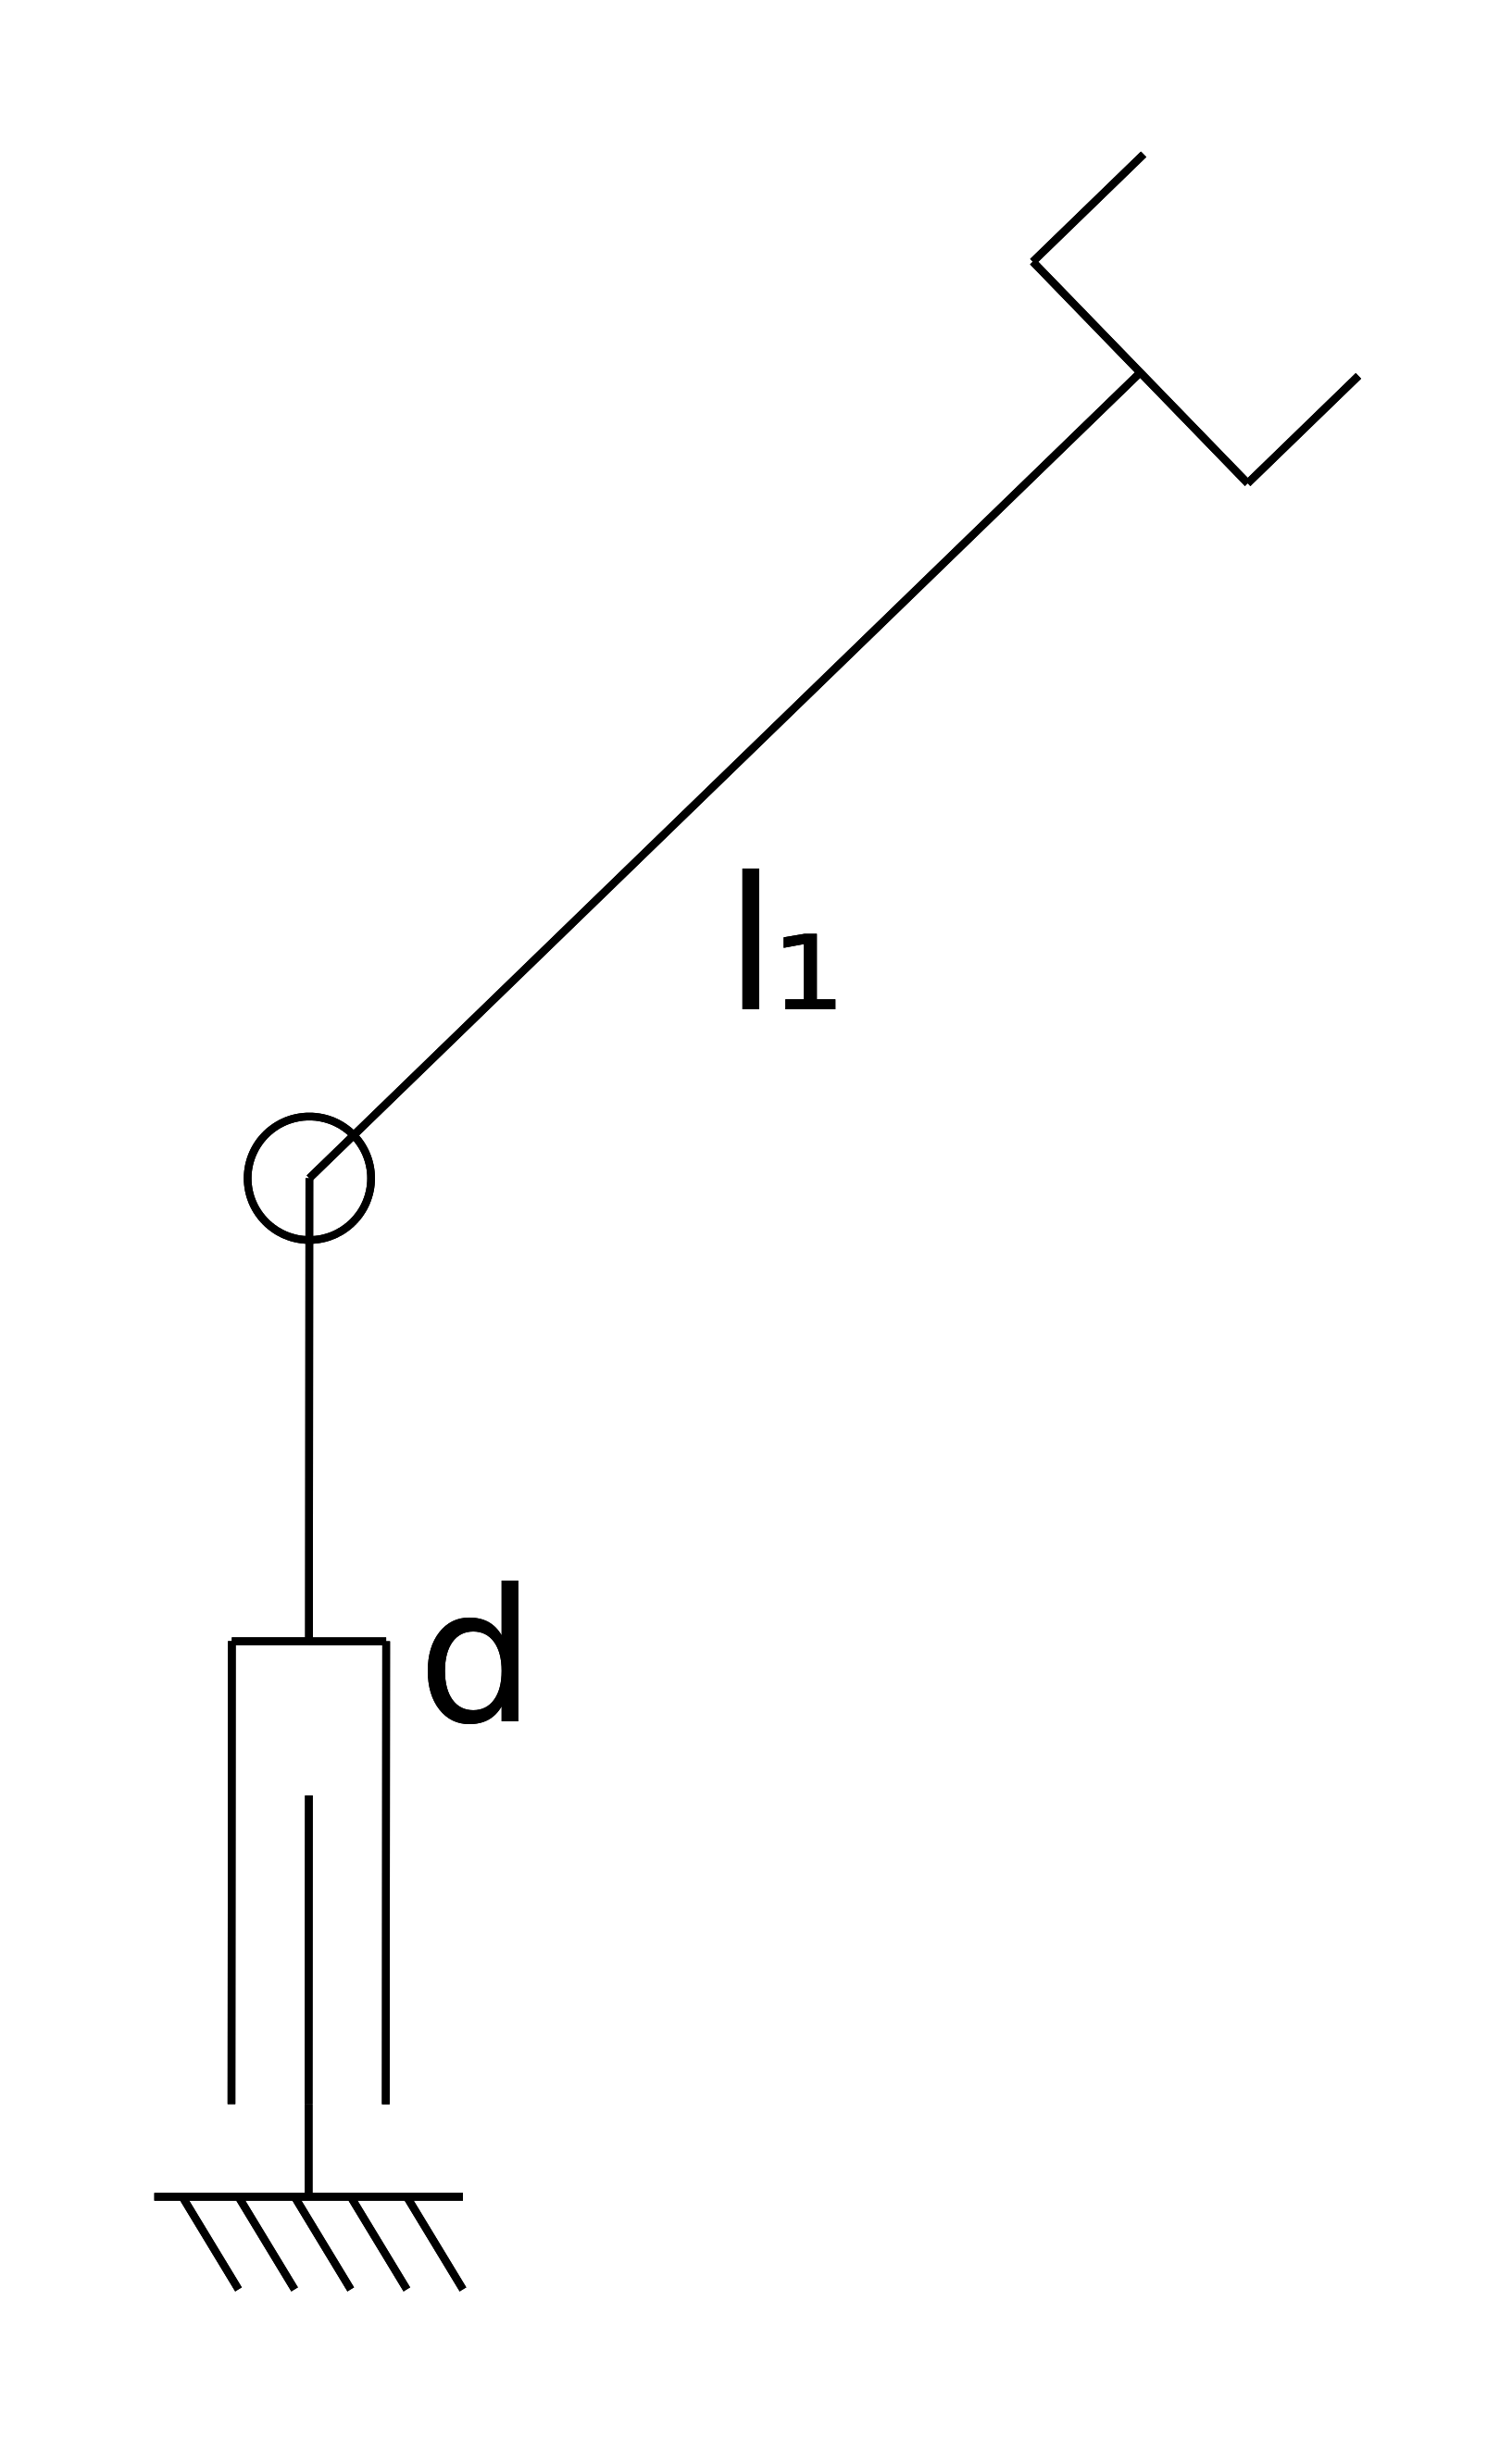
\includegraphics[width=1.5in]{generated_figures/robot_7.png}
    \end{center}
    Remember to use the frame conventions given in the background!

    \begin{tcolorbox}[height=13cm]
       % TODO: ENTER YOUR ANSWER HERE
    \end{tcolorbox}

    \newpage

    For the workspace, assume the prismatic joint can go from $d=0$ to $d=d_f$.
    
    \begin{tcolorbox}[height=10cm]
       % TODO: ENTER YOUR ANSWER HERE
    \end{tcolorbox}
    
    Draw a separate image for $d_f = l_1$ and $d_f > 2 l_1$.

    \begin{tcolorbox}[height=10cm]
       % TODO: ENTER YOUR ANSWER HERE
    \end{tcolorbox}

    \newpage

    \titledquestion{Forward Kinematics of a PR Arm}[9]
    Repeat problem 6 with the arm in the previous problem.

    \begin{parts}
        \part[1] \H{1}{0}
        
        \begin{tcolorbox}[height=10cm]
           % TODO: ENTER YOUR ANSWER HERE
        \end{tcolorbox}
        
        \part[1] \H{2}{1}
        
        \begin{tcolorbox}[height=10cm]
           % TODO: ENTER YOUR ANSWER HERE
        \end{tcolorbox}
        
        \newpage
        
        \part[1] \H{3}{2}
        
        \begin{tcolorbox}[height=10cm]
           % TODO: ENTER YOUR ANSWER HERE
        \end{tcolorbox}
        
        \part[1] \H{4}{3}
        
        \begin{tcolorbox}[height=10cm]
           % TODO: ENTER YOUR ANSWER HERE
        \end{tcolorbox}
        
        \newpage
        
        \part[1] \H{4}{0}, the transform from the end effector to the base
        frame (in terms of the previous transforms).
        
        \begin{tcolorbox}[height=20cm]
           % TODO: ENTER YOUR ANSWER HERE
        \end{tcolorbox}
        
    \end{parts}

    \newpage

    Substitute in the following values for the joint positions
    \smcolvec{d\\\th} for question 6 part f. Solving for both
    "nice" numbers and intermediate numbers will build 
    intuition of PR arm forward kinematics.

        \begin{parts}
            \part \smcolvec{0\\0}
            
            \begin{tcolorbox}[height=10cm]
               % TODO: ENTER YOUR ANSWER HERE
            \end{tcolorbox}
            
            \part \smcolvec{3\\\piover{2}}
            
            \begin{tcolorbox}[height=9cm]
               % TODO: ENTER YOUR ANSWER HERE
            \end{tcolorbox}
             \part \smcolvec{1\\-\piover{2}}
            
            \begin{tcolorbox}[height=10cm]
               % TODO: ENTER YOUR ANSWER HERE
            \end{tcolorbox}
            
            \part \smcolvec{3\\\piover{4}}
            
            \begin{tcolorbox}[height=10cm]
               % TODO: ENTER YOUR ANSWER HERE
            \end{tcolorbox}
            
        \end{parts}

    \newpage

    \titledquestion{Singularities}
    Consider the following RR arm:
    \begin{center}
    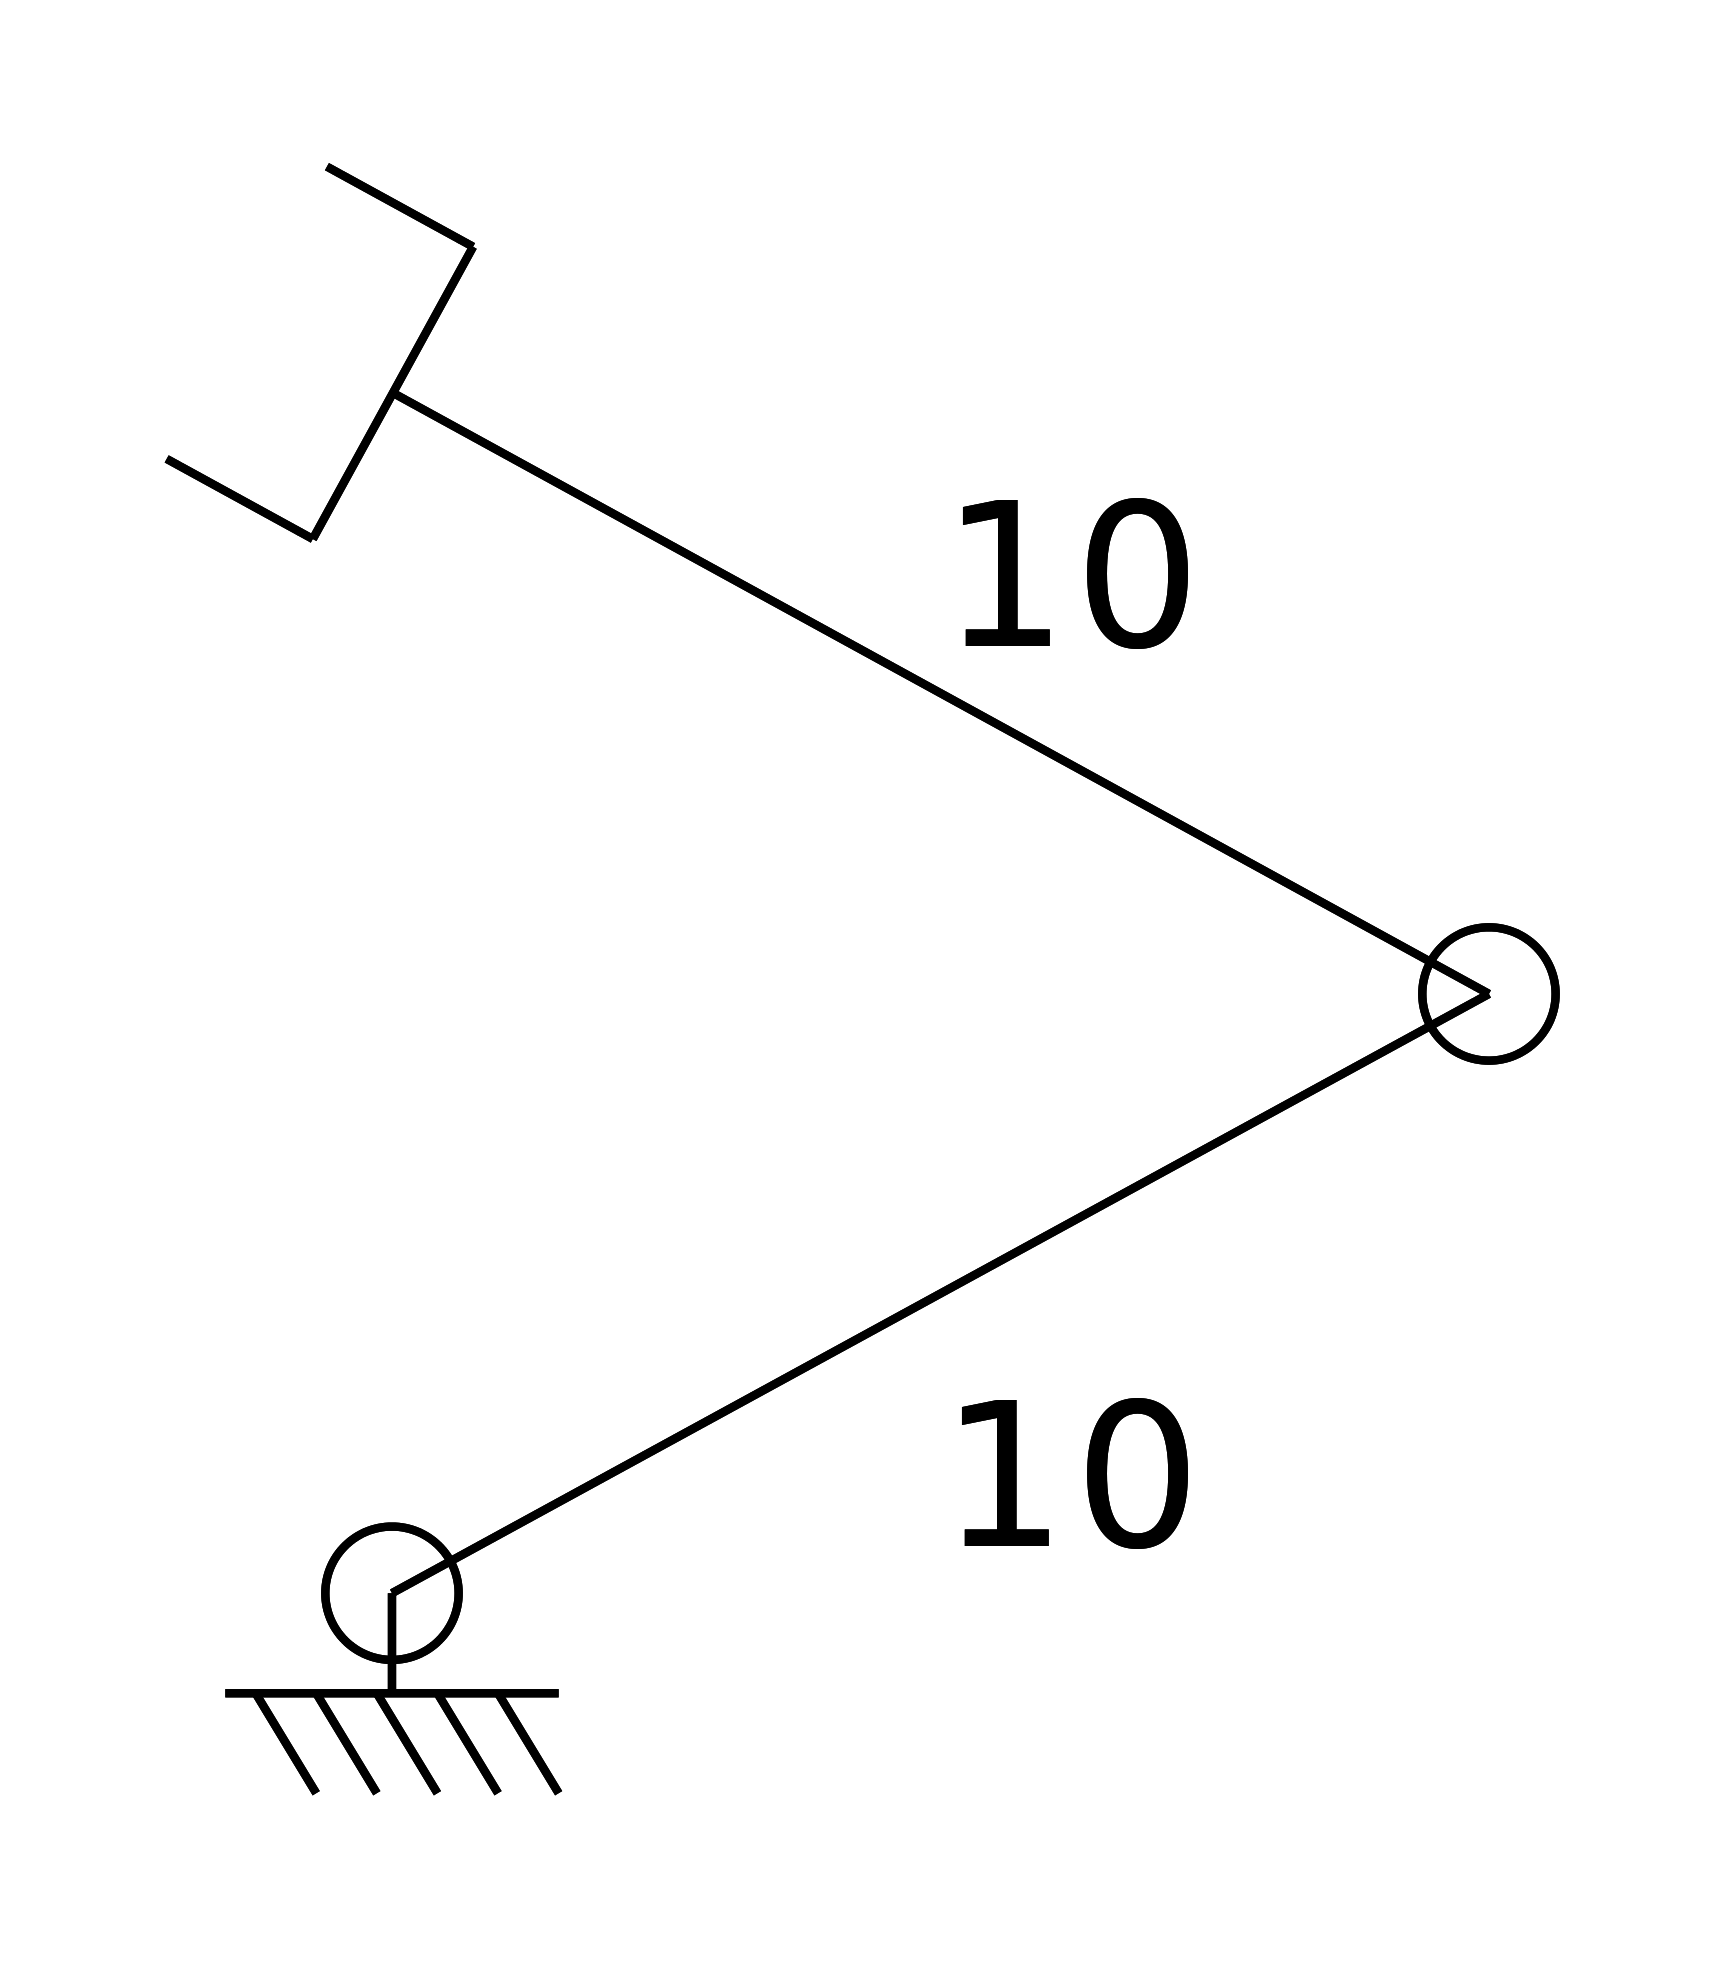
\includegraphics[width=1.5in]{generated_figures/robot_8.png}
    \end{center}

    Draw labeled plots. Please draw each part separately.

    For which \smcolvec{x\\y} in the workspace can \th=\smcolvec{\th[1]\\\th[2]}~have:
    \begin{parts}
        \part[2] Only 1 value?
        
        \begin{tcolorbox}[height=13cm]
           % TODO: ENTER YOUR ANSWER HERE
        \end{tcolorbox}
        
        \newpage
        
        \part[2] Exactly 2 values?
        
        \begin{tcolorbox}[height=20cm]
           % TODO: ENTER YOUR ANSWER HERE
        \end{tcolorbox}
            
        \newpage
            
        \part[2] Infinite values?
        
        \begin{tcolorbox}[height=20cm]
           % TODO: ENTER YOUR ANSWER HERE
        \end{tcolorbox}
            
            
    \end{parts}

    

\end{questions}

\feedback{\feedbackURL}

\section{Code Questions}

In these problems, we'll analytically test some of the work from the previous
section.

%Download the assignment handout from the \href{\resourceURL}{course website}. 
Copy the Code Handout folder to some location of your choice. Open Matlab and navigate to that location. Whenever you work on the assignment, go into this directory and run \verb!setup.m!.

\begin{questions}
    \titledquestion{Forward Kinematics}[10]

    Begin by opening the \verb!ex_01! directory in Matlab.

    In this exercise, you must fill out the \verb!forward_kinematics_RR.m! file.
    When completed correctly, this function should define the forward kinematics
    for an RR arm with angles \verb!theta_1! and \verb!theta_2!, and link
    lengths $l_1$ and $l_2$ (these values are given in the
    \verb!forward_kinematics_RR.m! file).

    You will define four matrices in this file: \H{1}{0}, \H{2}{0}, \H{3}{0},
    and \H{4}{0}.  Use the following conventions for the frames (hint: these
    should match the frames for problem 6 in the written section).

    \begin{itemize}
        \item The base frame of the entire robot is \frame{0}.
        \item The starting frame for the first link is \frame{1}.
        \item The frame at the end of the first link is \frame{2}.
        \item The starting frame for the second link is \frame{3}.
        \item The end effector frame is \frame{4}.

        \item In the code, transform \verb!H_i_j! refers to the transform \H{i}{j}.
    \end{itemize}

    Confirm that you have the correct forward kinematics before moving to the
    next problem.  First, we suggest testing a couple of simple cases -- for
    example, angles of $0$ or $\pi / 2$ -- and ensuring the resulting
    transformations properly transform points in the respective frames to the
    base frame.

    We have also provided a validation script to test your kinematics:

    \begin{itemize}
        \item Run the script \verb!sample_path!.  This loads a log of the robot
            moving, and plots the end effector trajectory generated by your
            kinematics against ground truth end effector positions.  Verify that
            these paths match.
    \end{itemize}

    Before continuing, ensure that the kinematics are correct using the above
    script!

    \titledquestion{Workspace Analysis}[10]

    Begin by opening the \verb!ex_02! directory in Matlab.

    In this exercise, you will create a workspace analysis for a PR arm.

    First, run the \verb!workspace_analysis_RR.m! file. This is a function which
    takes one argument that is a vector of link lengths $l_1$ and $l_2$.
    Executing this should generate a figure showing the end effector positions
    for a complete sweep of joint angles for an RR arm.  Compare this to the
    results from problem 6.

    Your task is to create a \verb!workspace_analysis_PR.m! file, which generates the workspace
    analysis for the PR arm you studied in problem 7 in the written section. Use the RR analysis
    code as a starting point for this PR analysis. As before, the prismatic joint can go from $d 
    = 0$ to $d = d_f$. Note that the input for this function should be the link length $l_1$.

    The deliverables for this problem are two figures, saved as MATLAB .fig files (click file->save from the figure menu):

    \begin{itemize}
        \item For the first, let $l_1 = 1$, and $d_f = 1$. Save this as
	\verb!workspace_pr_1.fig!
        \item For the second, let $l_1 = 0.5$, and $d_f = 2$. Save this as
	\verb!workspace_pr_2.fig!
    \end{itemize}

    Check that these match the results that you gave in problem 7!

\end{questions}

\section{Hands-On Questions}

\begin{questions}
    \titledquestion{Tracing Objects with an Arm}[10]

    Begin by opening the \verb!ex_03! directory in Matlab.

    In this section, we will verify that you can indeed connect to the robot
    arm, and that your forward kinematics are correct.

    First, follow the directions on Piazza to begin Remote Access. Then, once you have 
    MATLAB open on the remote desktop, type \verb!HebiLookup! into the MATLAB 
    command line, and ensure there are two modules (joint1 and joint2) listed 
    in the table of available modules. If not, notify the TA to plug in wall ethernet
    cord to the desktop first and the robot ethernet cord second.

    With the forward kinematics you've written, you should be able to run
    \verb!trace_object!, which takes control of the robot arm, and puts it in
    a passive mode. This should also bring up a live plot of the robot arm,
    using your forward
    kinematics to properly show the robot's position and configuration.  Ask the
    TA to move the arm around.  Does your code work properly?

    When you're ready, hit spacebar to begin recording the robot's motion.  Ask the TA to use
    the arm to trace the star shape taped to the table.  When you're done, hit
    space bar once again.  If the plot that comes up is shaped like you expect,
    you've correctly completed the lab!  If not, double check your forward
    kinematics.

    Whenever you use the spacebar to load a plot, you create a file called
    \verb!star_trace.hebilog!.  This is your deliverable for this question.
    MAKE SURE TO PUSH EVERYTHING TO YOUR PRIVATE GITHUB REPOSITORY!

    \titledquestion{Submission}
        After you pull everything back onto your laptop, check that you have everythin to submit.
        To submit, run \verb!create_submission.m!.  It will first check that
        your submitted files run without error, and perform a small sanity
        check. Note, this is not going to grade your submission!  The function
        will create a file called \verb!handin-1.tar.gz!. 
\end{questions}

\begin{submissionChecklist}
		\item Create a PDF of your answers to the written questions with the name \verb!writeup.pdf!.
		\item Make sure you have \verb!writeup.pdf! in the same folder as the \verb!create_submission.m! script.
		\item Run \verb!create_submission.m! in Matlab.
		\item Upload \verb!handin-1.tar.gz! to Canvas
		\item Upload your \verb!writeup.pdf! to Gradescope.
		\item After completing the entire assignment, fill out the feedback
		form\footnotemark.
	%~and make sure to add the submission code as the answer to the feedback section. 
		\footnotetext{\texttt{\href{\feedbackURL}{\feedbackURL}}}
	\end{submissionChecklist}

\end{document}
